\documentclass[12pt,a4paper]{article}
\usepackage[a4paper,top=1.5cm, bottom=1.5cm, left=1.5cm, right=1.5cm]{geometry}
\usepackage[T2A]{fontenc}
\usepackage[utf8]{inputenc}
\usepackage[russian]{babel}
\usepackage{amsmath}
\usepackage{amssymb}
\usepackage{graphicx}
\usepackage{floatrow}
\usepackage{booktabs}
\usepackage{wrapfig}
\usepackage{indentfirst}
\usepackage{lipsum}
\usepackage{subcaption}
\usepackage{float}
\usepackage{enumitem}
\restylefloat{table}

\newcommand{\figref}[1]{(см. рис. \ref{#1})}
\newcommand{\e}[1]{\text{$\cdot10^{#1}$}}

\title{Работа №26\\ Цифровые фильтры}
\author{Симанкович Александр \\ Б01-104}
\date{\today}

\begin{document}
	\maketitle	
	
	\subsection*{1. Ознакомительные шаги}
	
	Рассмотрим спектры оцифрованных сигналов.
	

	
	\begin{figure}[H]
		\centering
		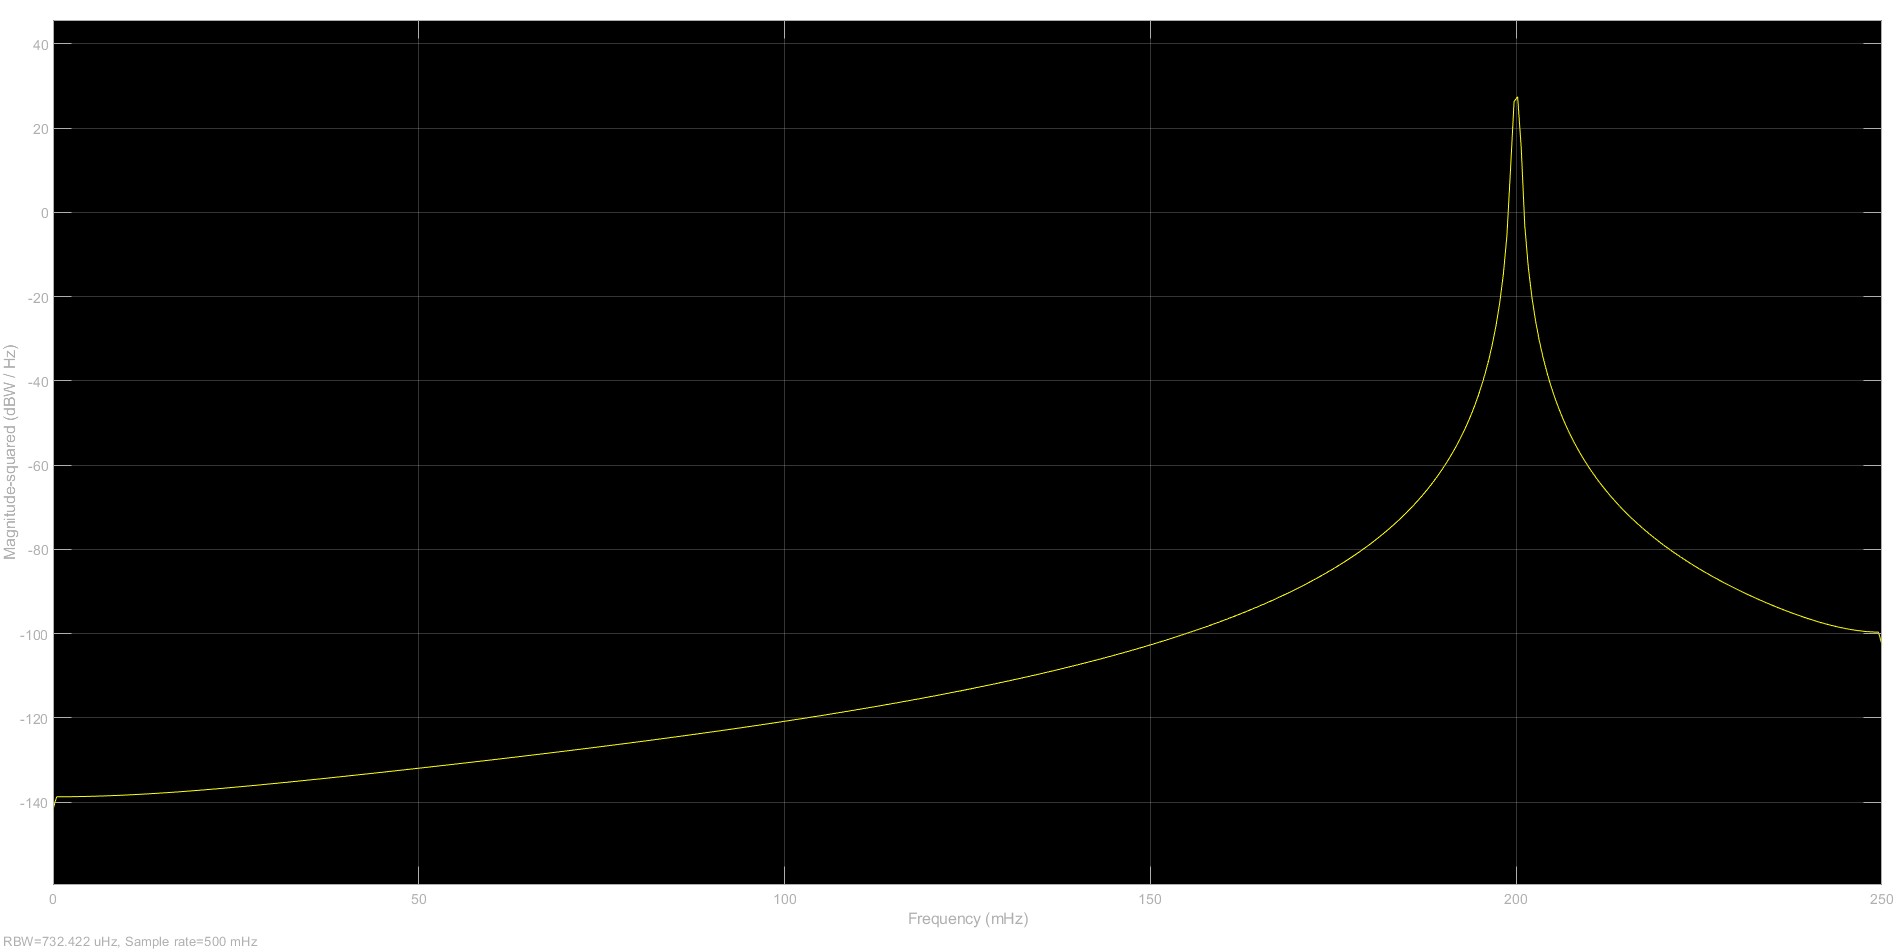
\includegraphics[width=1.0\linewidth]{res/1_spectrum_wdec.png}
		\caption{Спектр оцифрованного синусоидального сигнала: с дециматором }
	\end{figure}
	
	\begin{figure}[H]
		\centering
		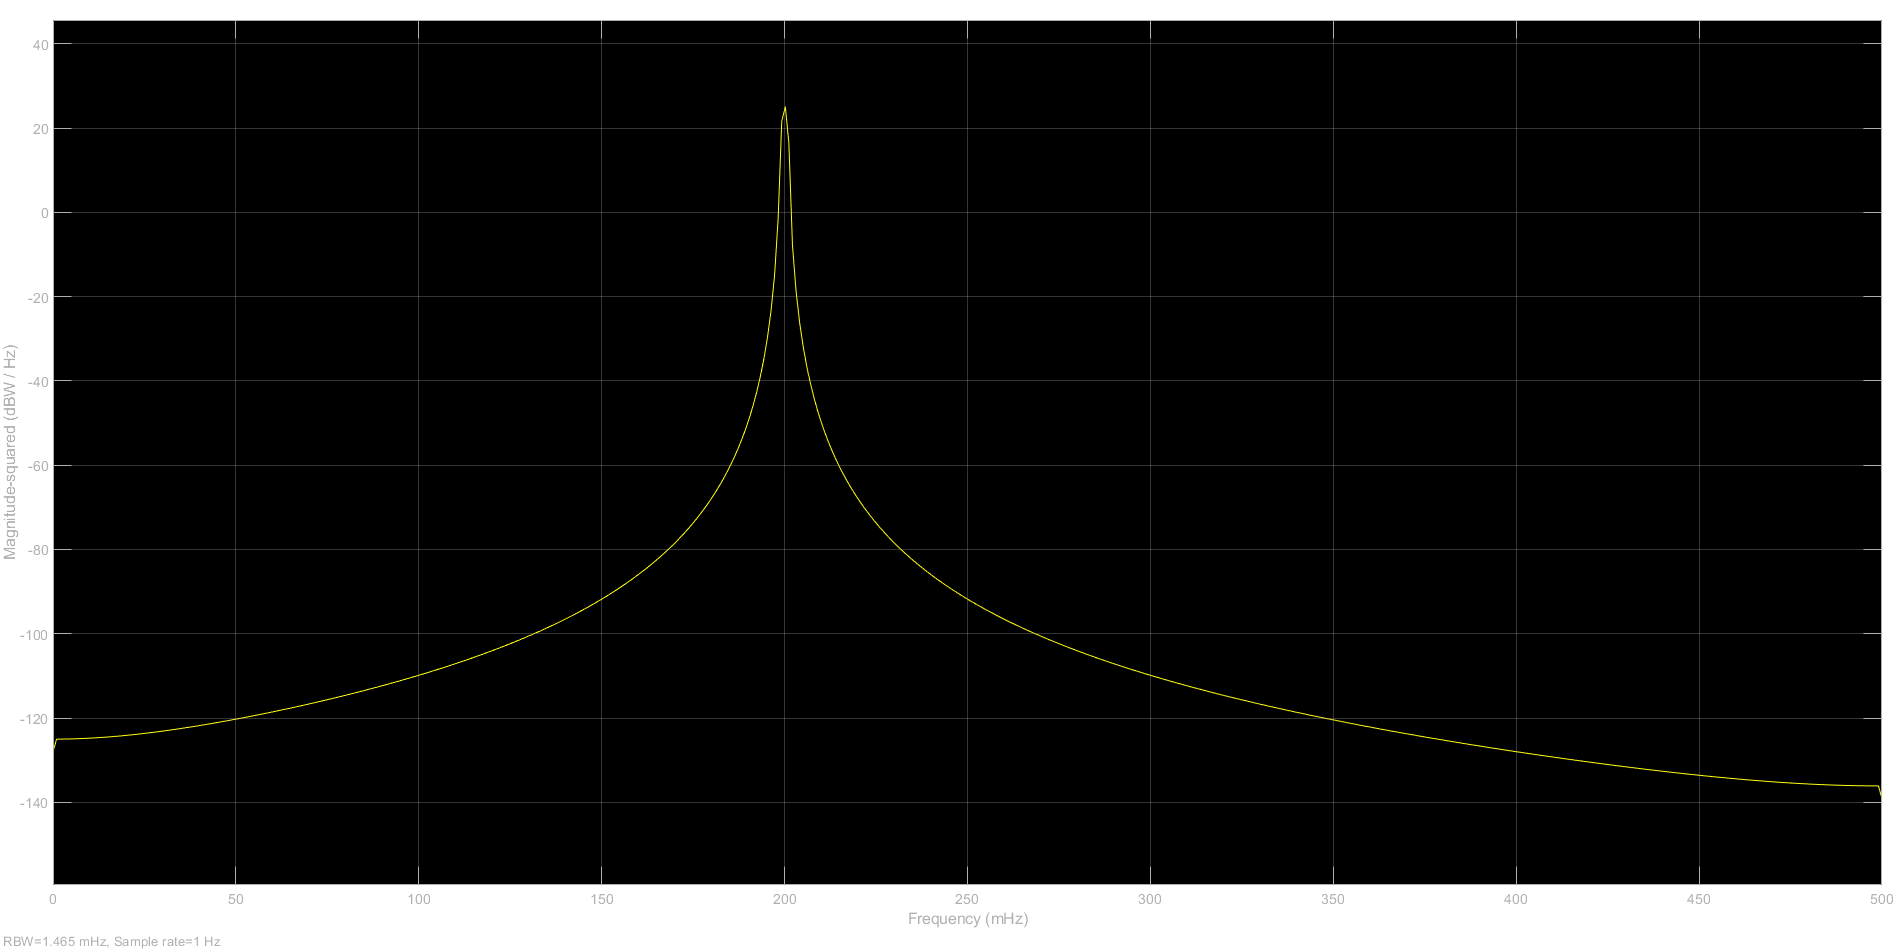
\includegraphics[width=1.0\linewidth]{res/1_spectrum_wodec.png}
		\caption{Спектр оцифрованного синусоидального сигнала: без дециматора }
	\end{figure}

	\begin{figure}[H]
		\centering
		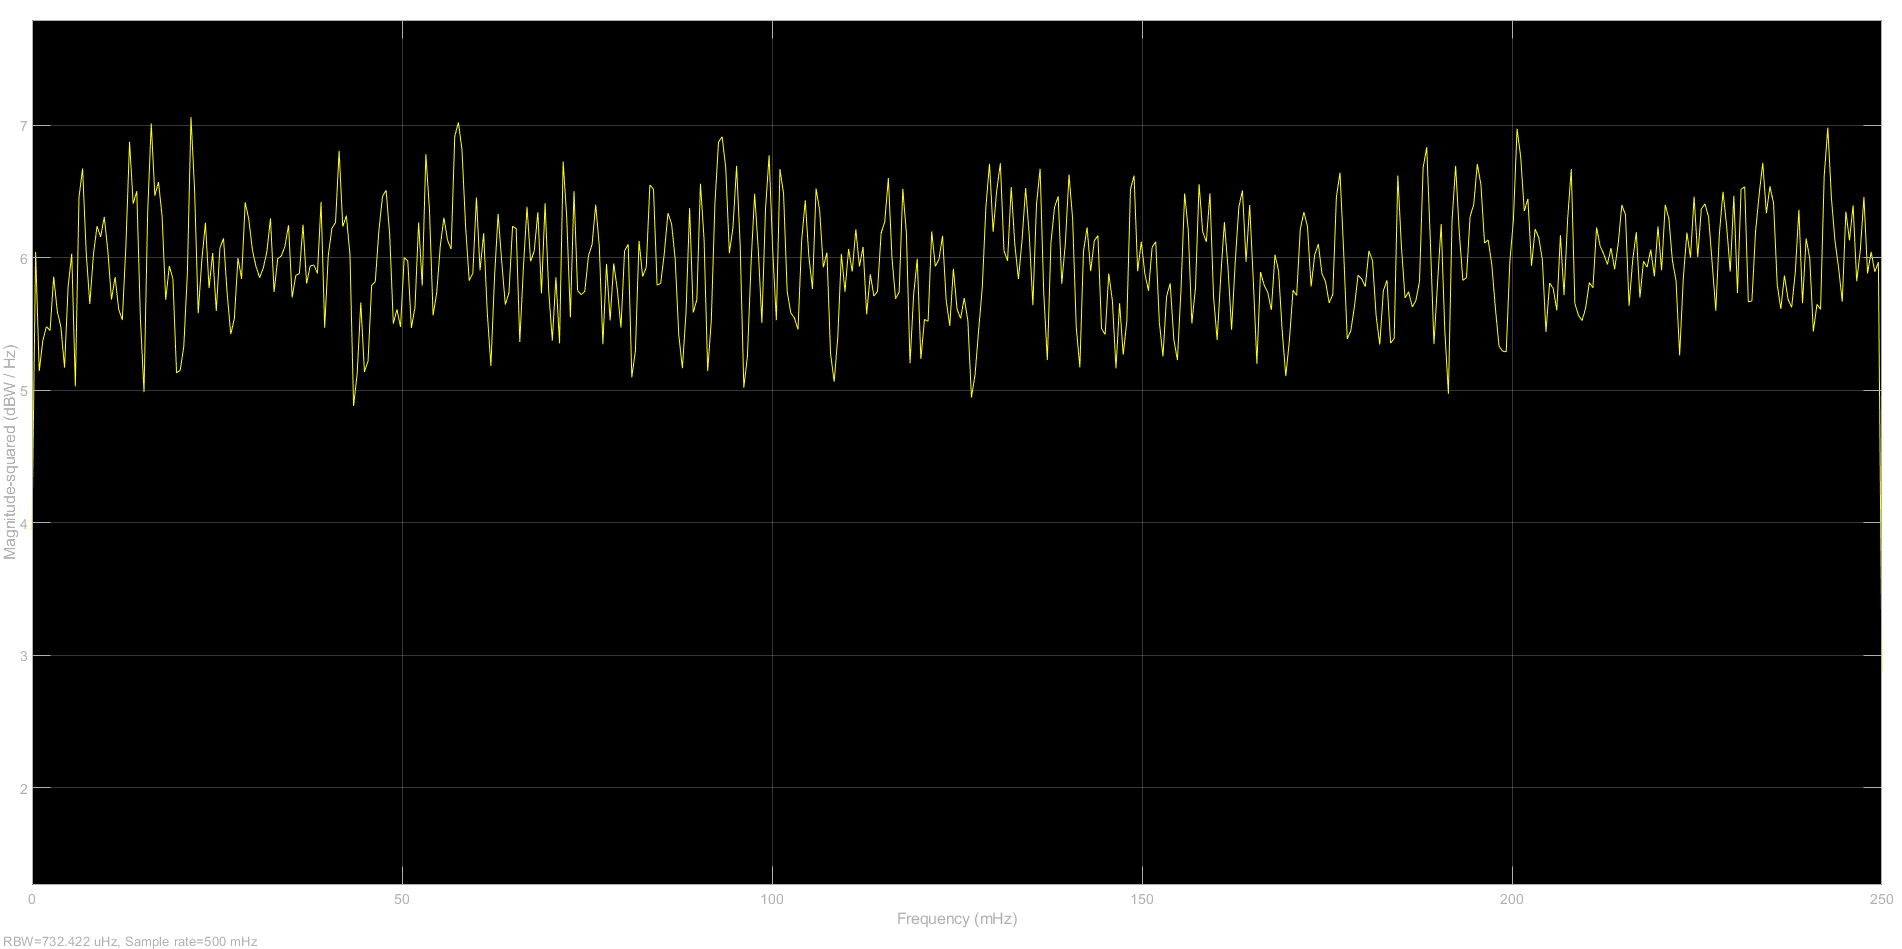
\includegraphics[width=1.0\linewidth]{res/1_noise_wdec.png}
		\caption{Спектр оцифрованного белого шума: с дециматором}
	\end{figure}
	
	\begin{figure}[H]
		\centering
		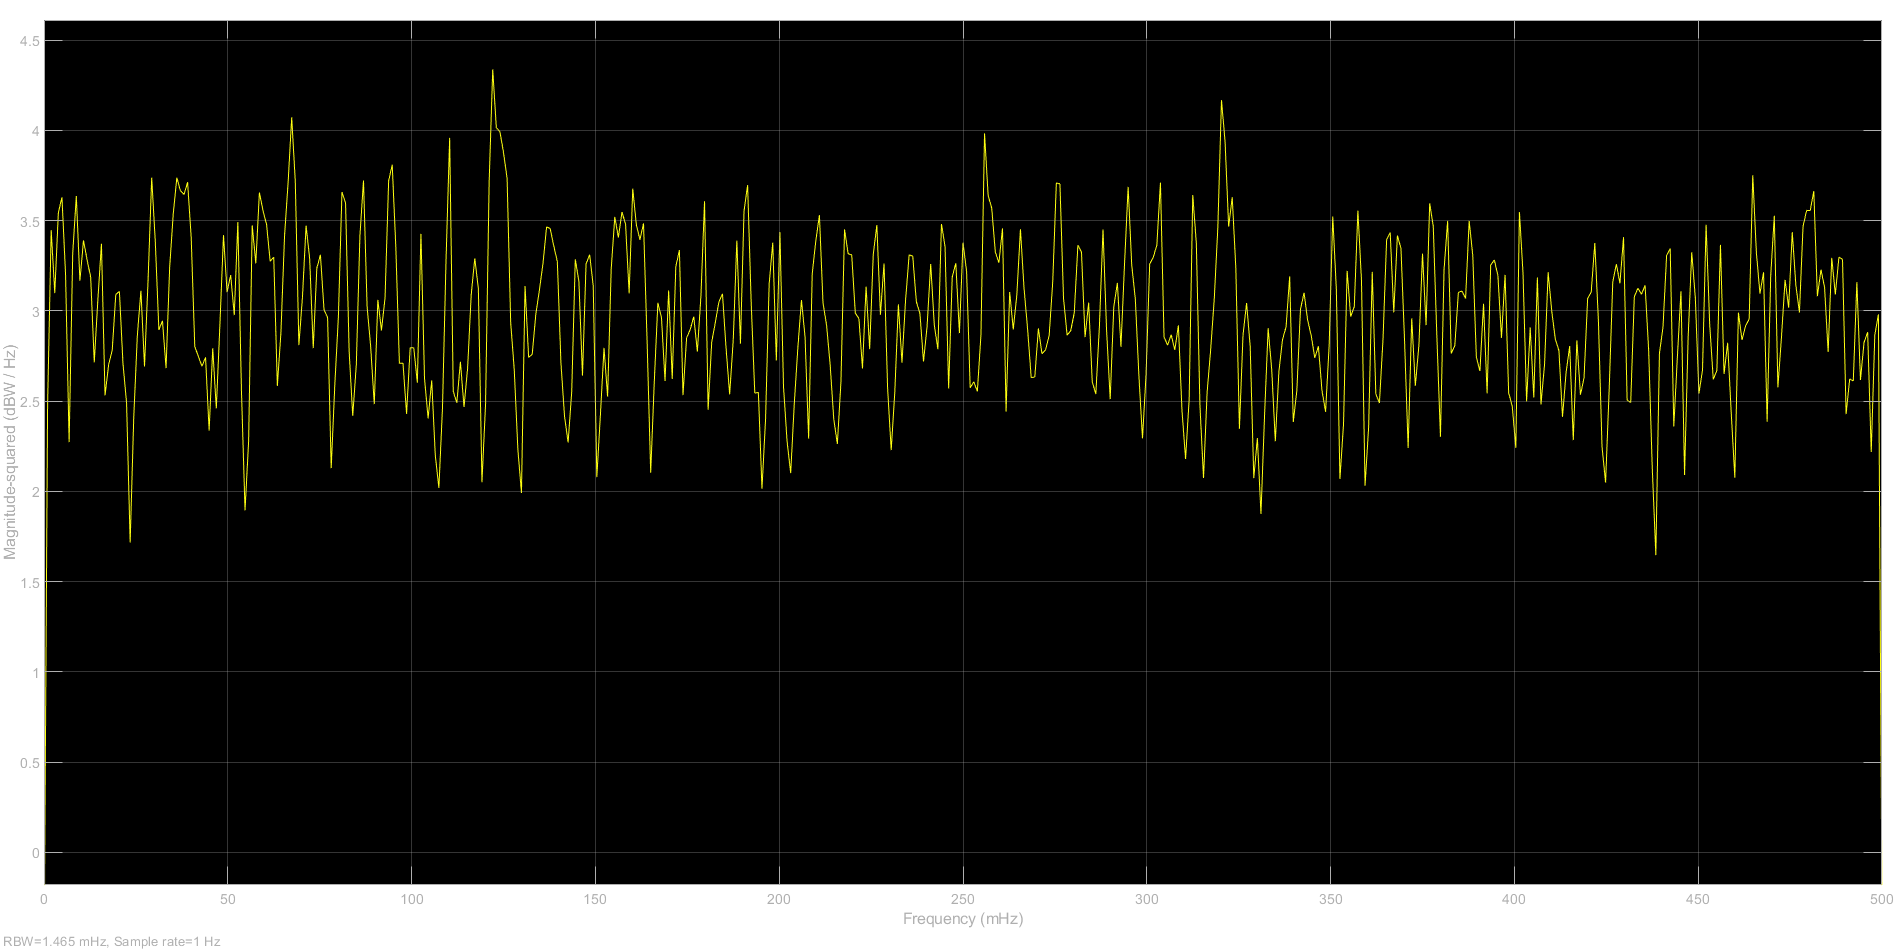
\includegraphics[width=1.0\linewidth]{res/1_noise_wodec.png}
		\caption{Спектр оцифрованного белого шума: без дециматорома}
	\end{figure}
	
	Отличие уровней на $10 \log 2 = 3 \; dB$ обусловлено сужением полосы с 1 до $\frac{1}{2}$.

	\begin{figure}[H]
		\centering
		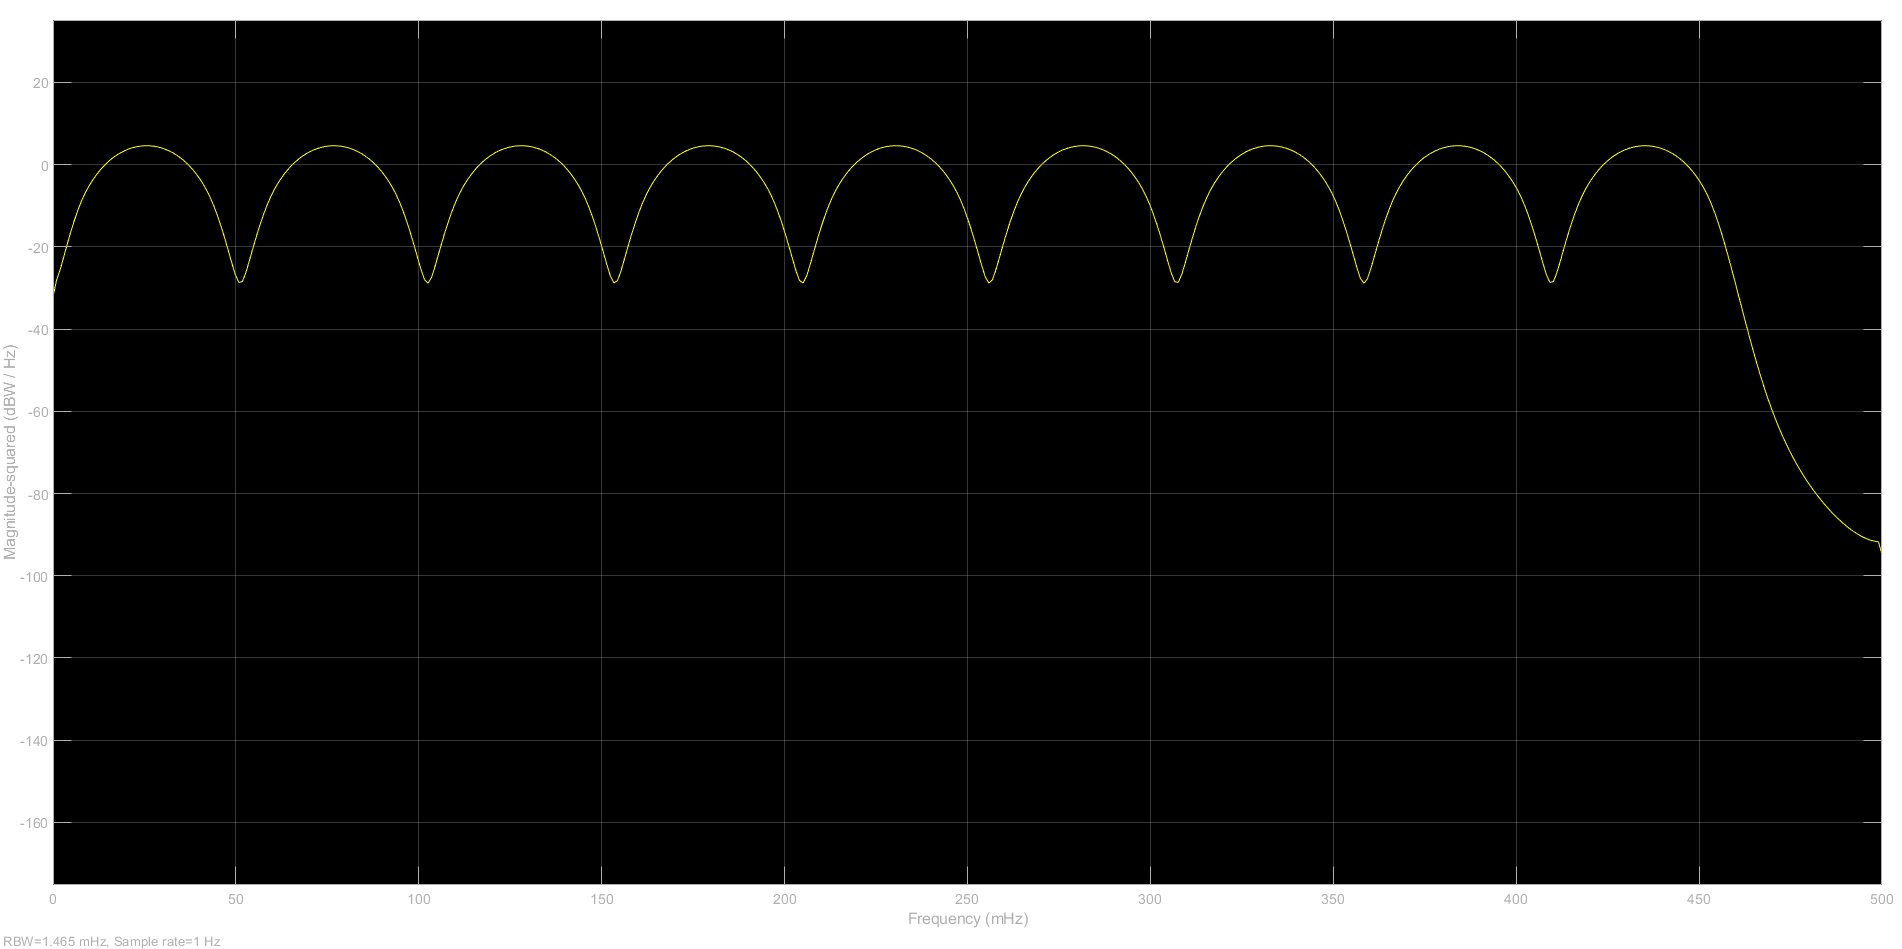
\includegraphics[width=1.0\linewidth]{res/1_chirp.png}
		\caption{Спектр свип-генератора: линейно от 0 до 0.5 за 10000 тактов}
	\end{figure}
	
	\subsection*{2. Фильтры первого порядка}
	
	Рассмотрим цифровой фильтр с параметрами $h = [1], g = [1, -0.7]$:
	
	\begin{figure}[H]
		\centering
		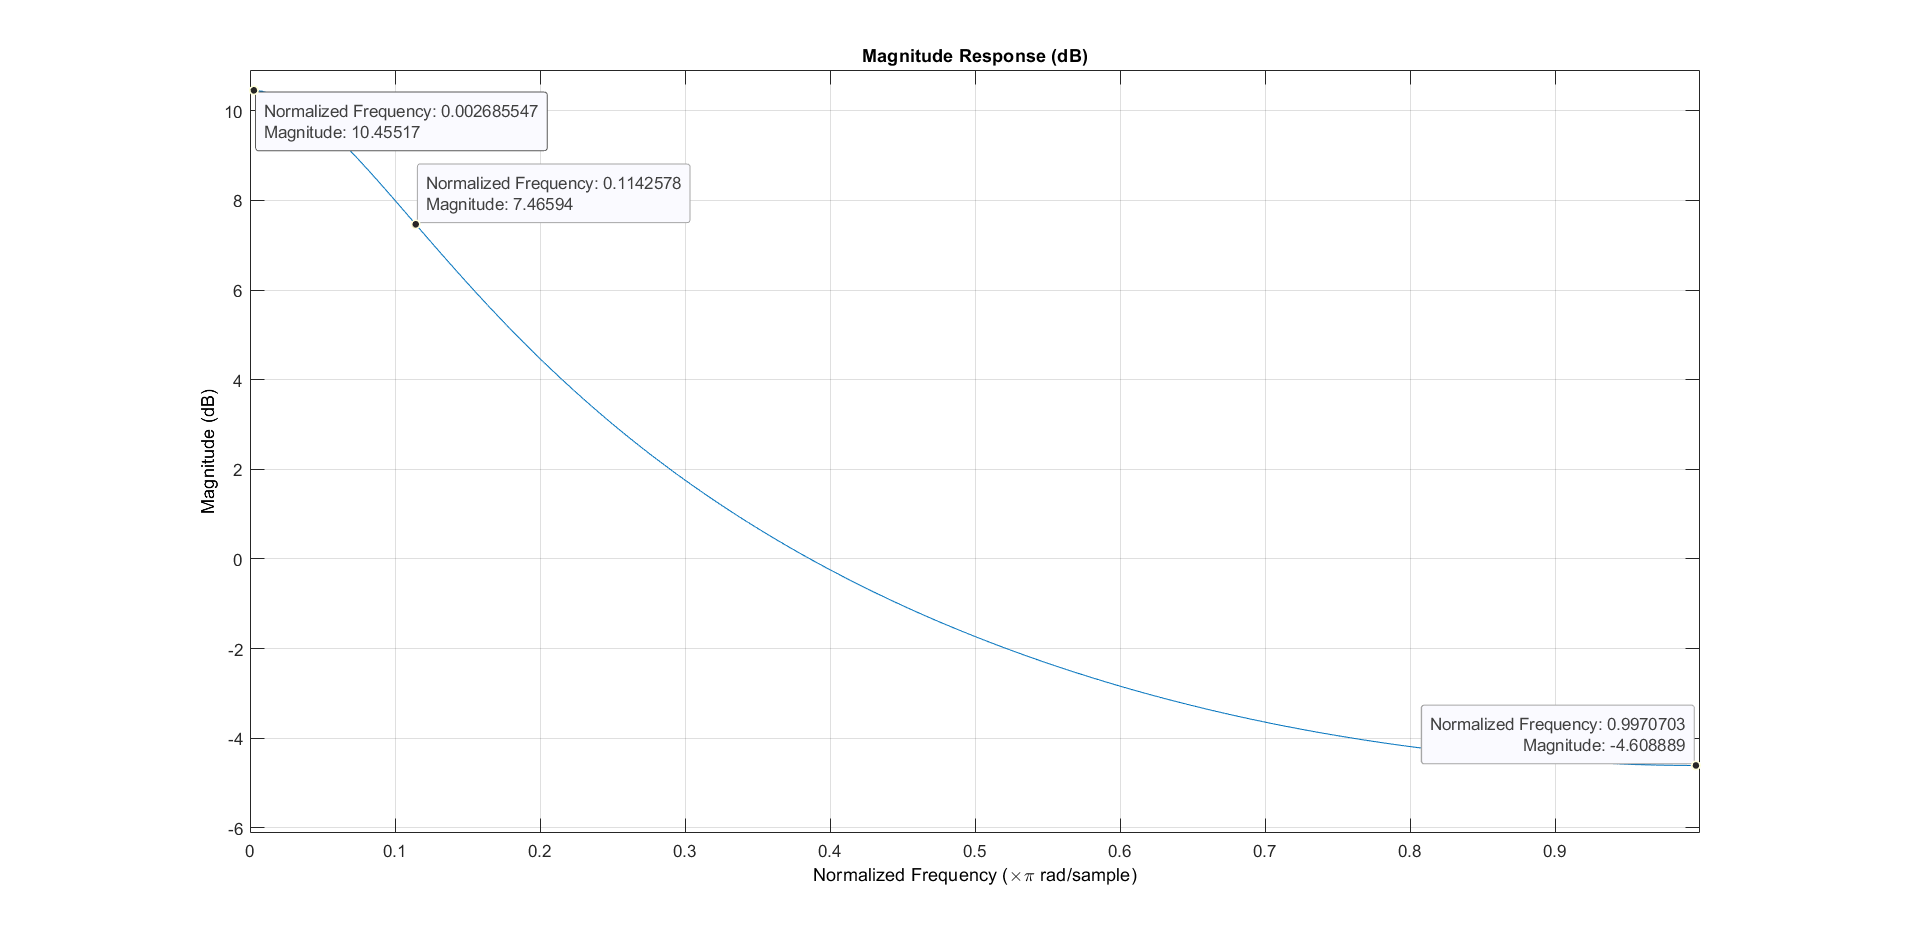
\includegraphics[width=1.0\linewidth]{res/2_2_ach.png}
		\caption{Спектр интегрирующего звена}
	\end{figure}

	$$K(0) = 3.33 \qquad K(1/2) = 0.59 \qquad f_0 = 0.055 \qquad \tau = 3 \Rightarrow f_0 = \frac{1}{2 \pi \tau} = 0.053.$$

	Подадим на вход гармонический сигнал:
	
	\begin{figure}[H]
		\centering
		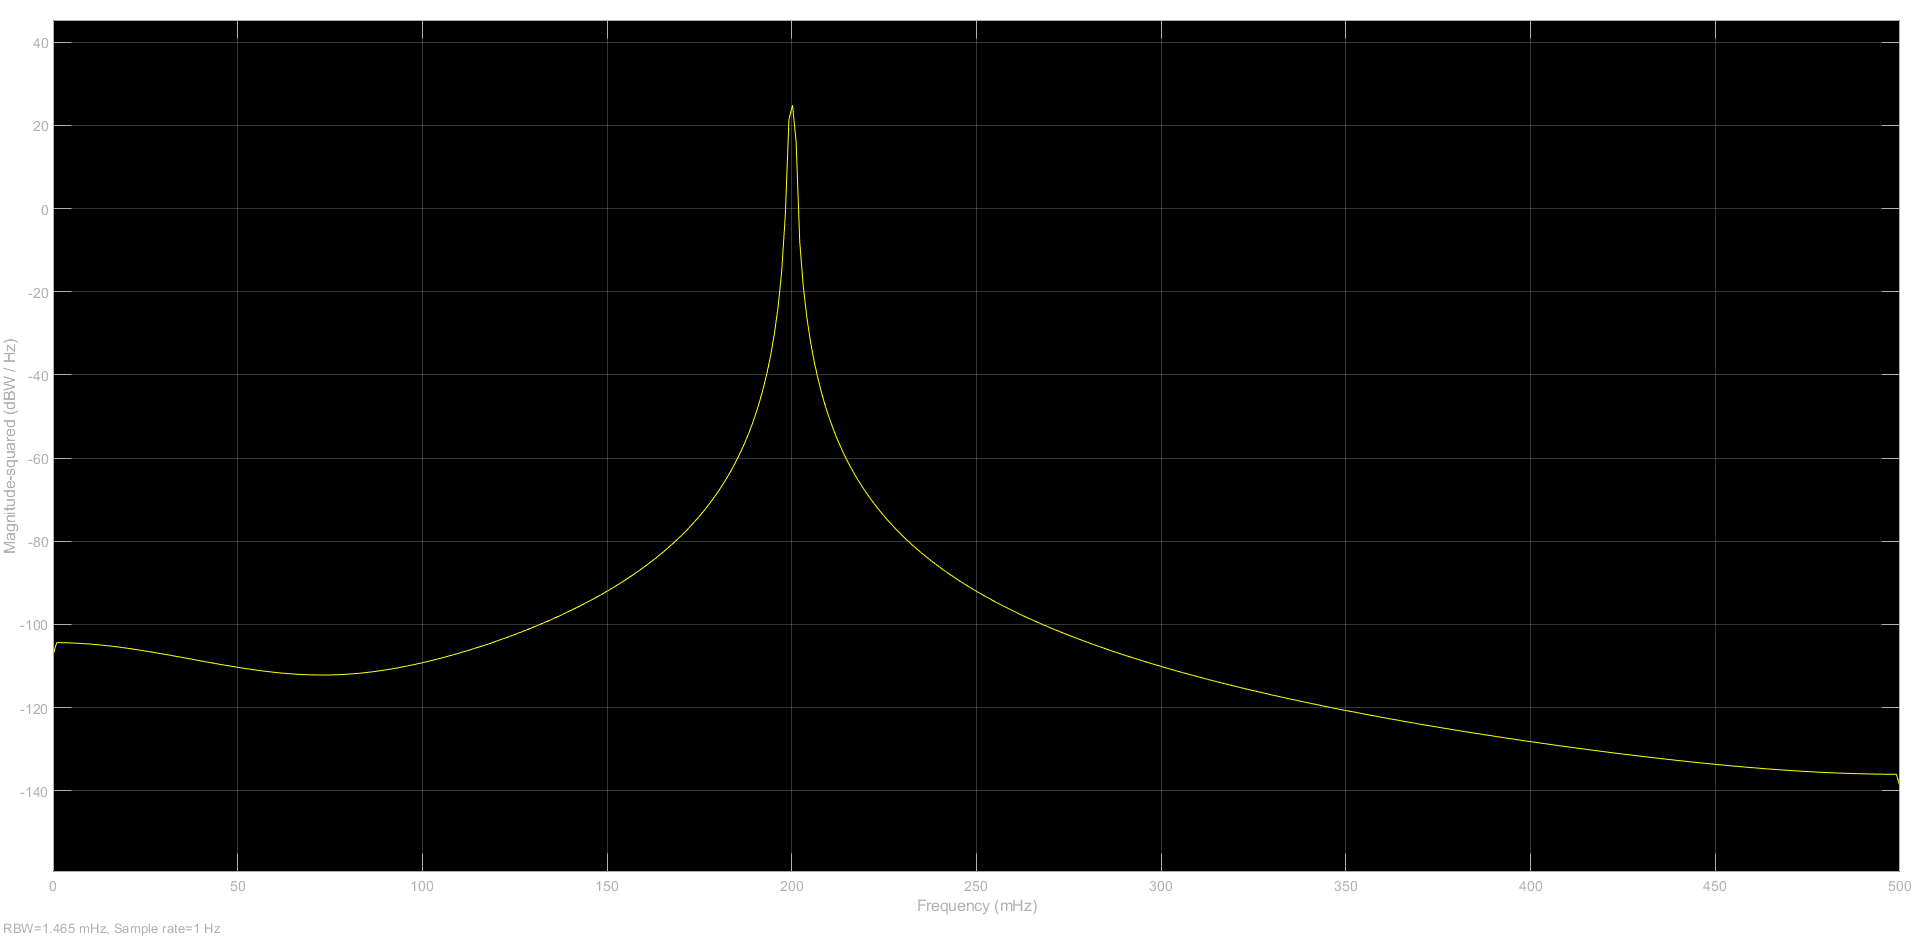
\includegraphics[width=1.0\linewidth]{res/2_4_sin.png}
		\caption{Спектр оцифрованного синусоидального сигнала}
	\end{figure}

	Настроив на нужные частоты получим коэффиценты передачи:
	$$K(0.05/2) = 34 \; dB \qquad K(0.95/2) = 19 \; dB$$.

	Рассмотрим осциллограммы синусоид с частотами $0.95/2$ и $0.05/2$.
	
	\begin{figure}[H]
		\centering
		\begin{minipage}[b]{.5\textwidth}
			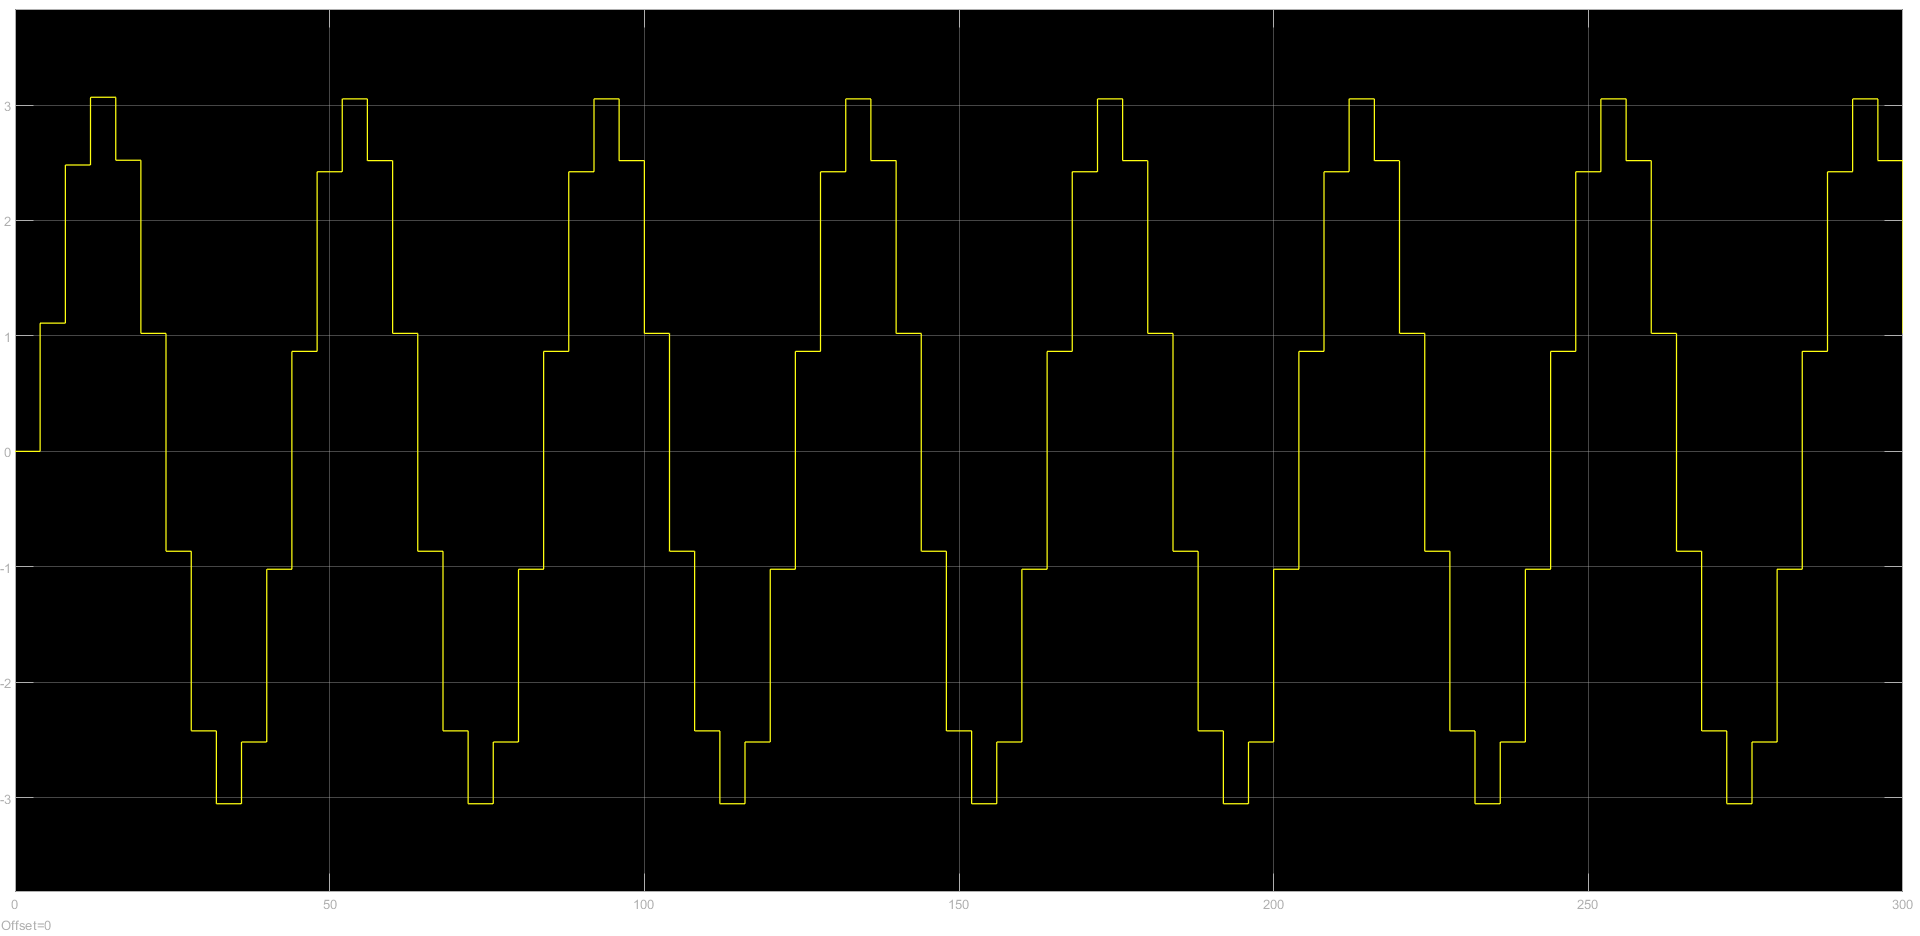
\includegraphics[width=0.9\linewidth]{res/2_5_005.png}
		\end{minipage}%
		\begin{minipage}[b]{.5\textwidth}
			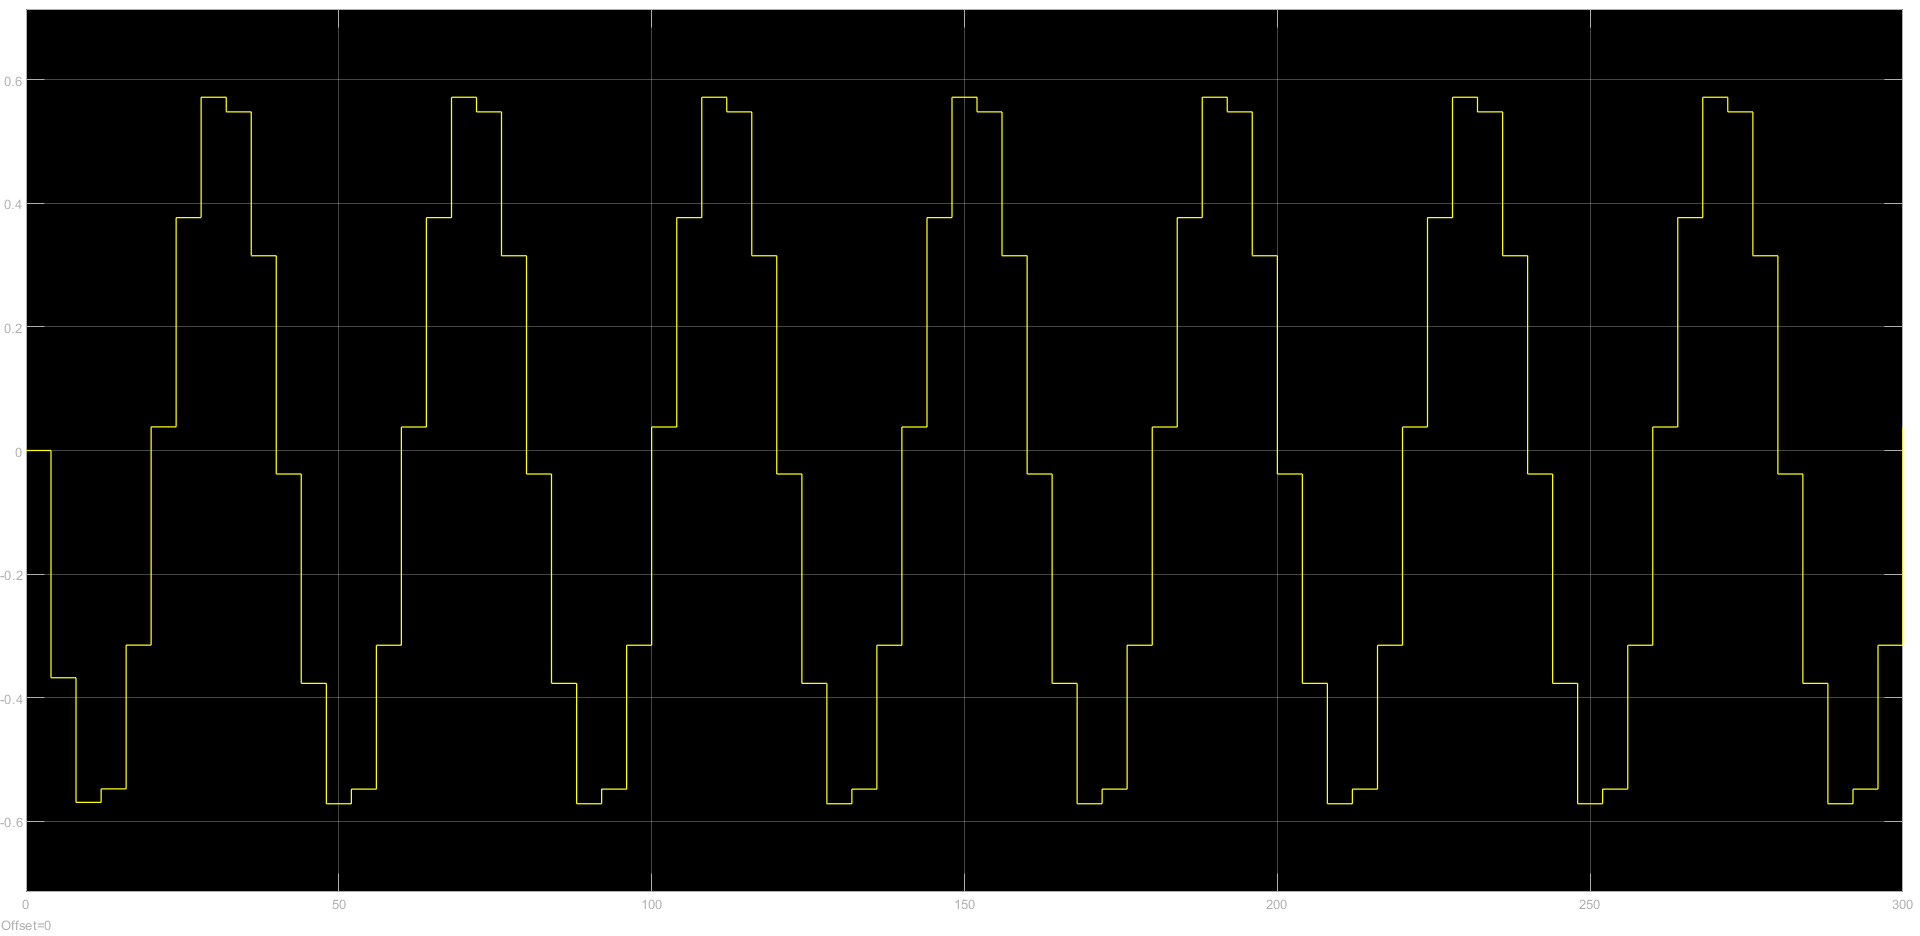
\includegraphics[width=0.9\linewidth]{res/2_5_095.png}
		\end{minipage}
		\caption*{Осциллограммы сигналов после фильтра: $K = 0.05/2$ (слева), $K = 0.95/2$ (справа)}
	\end{figure}

	Соотношение амплитуд $5.6$, что сходится с усилениями.
	
	Рассмотрим спектры шума до и после фильтра:
	
	\begin{figure}[H]
		\centering
		\begin{minipage}[b]{.5\textwidth}
			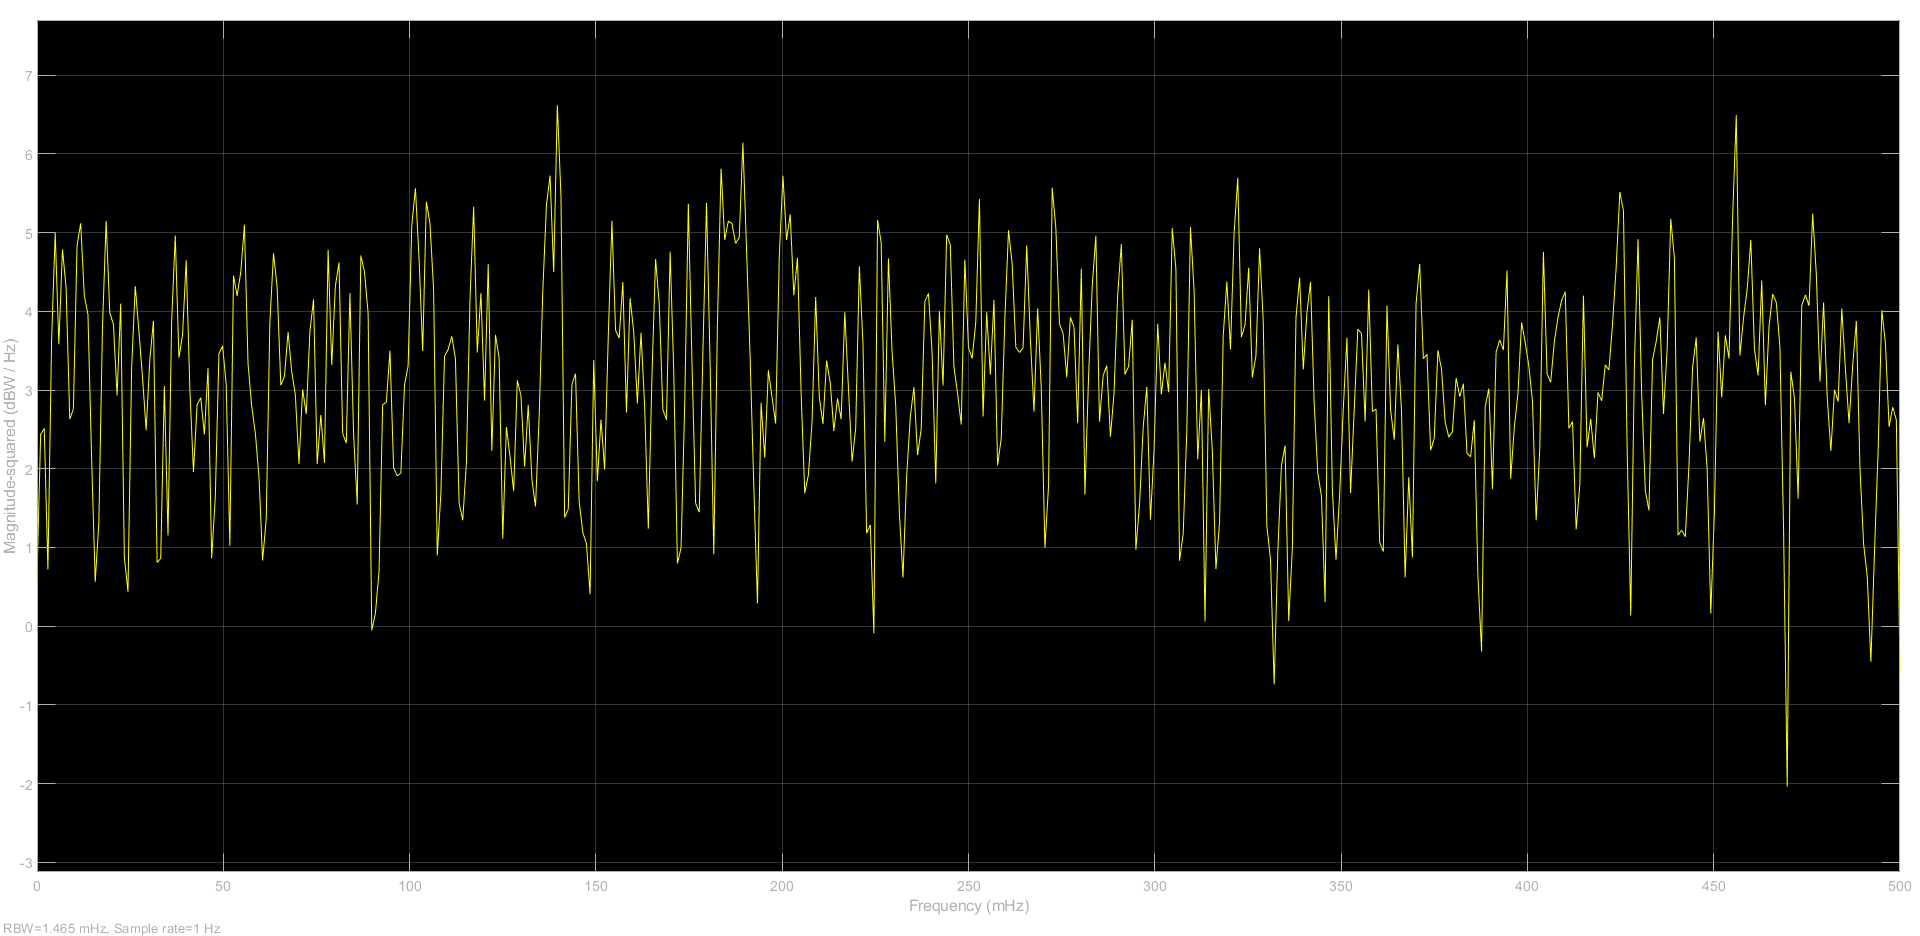
\includegraphics[width=0.9\linewidth]{res/2_6_before.png}
		\end{minipage}%
		\begin{minipage}[b]{.5\textwidth}
			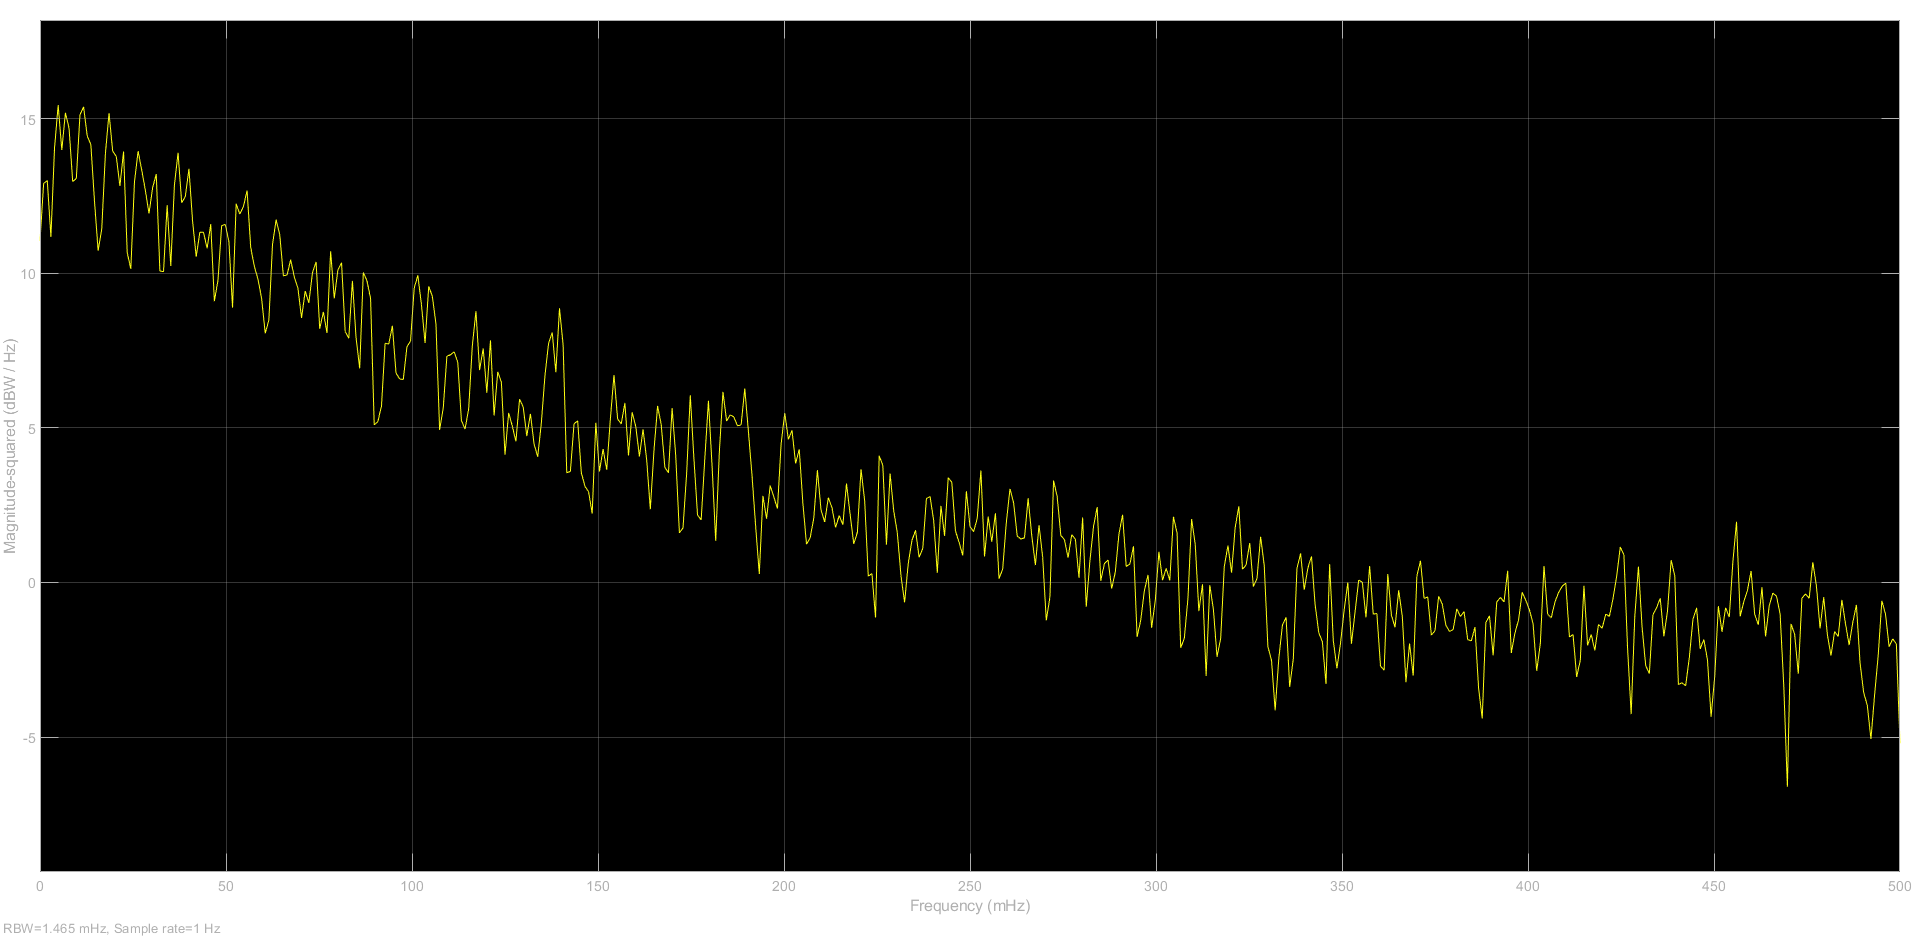
\includegraphics[width=0.9\linewidth]{res/2_6_after.png}
		\end{minipage}
		\caption*{Спектры шума: на входе (слева) и на выходе (справа)}
	\end{figure}
	
	В середине полосы Найквиста $\pm 250$ уровни шума одинаковы. На границе $\pm 500$ уровень до $3 \; dB$, уровень после $-3 \; dB$.
	
	Изучим идеальный интегратор с $\mu = 1$: $h = [1]$, $g = [1, -0.7]$:
	
	\begin{figure}[H]
		\centering
		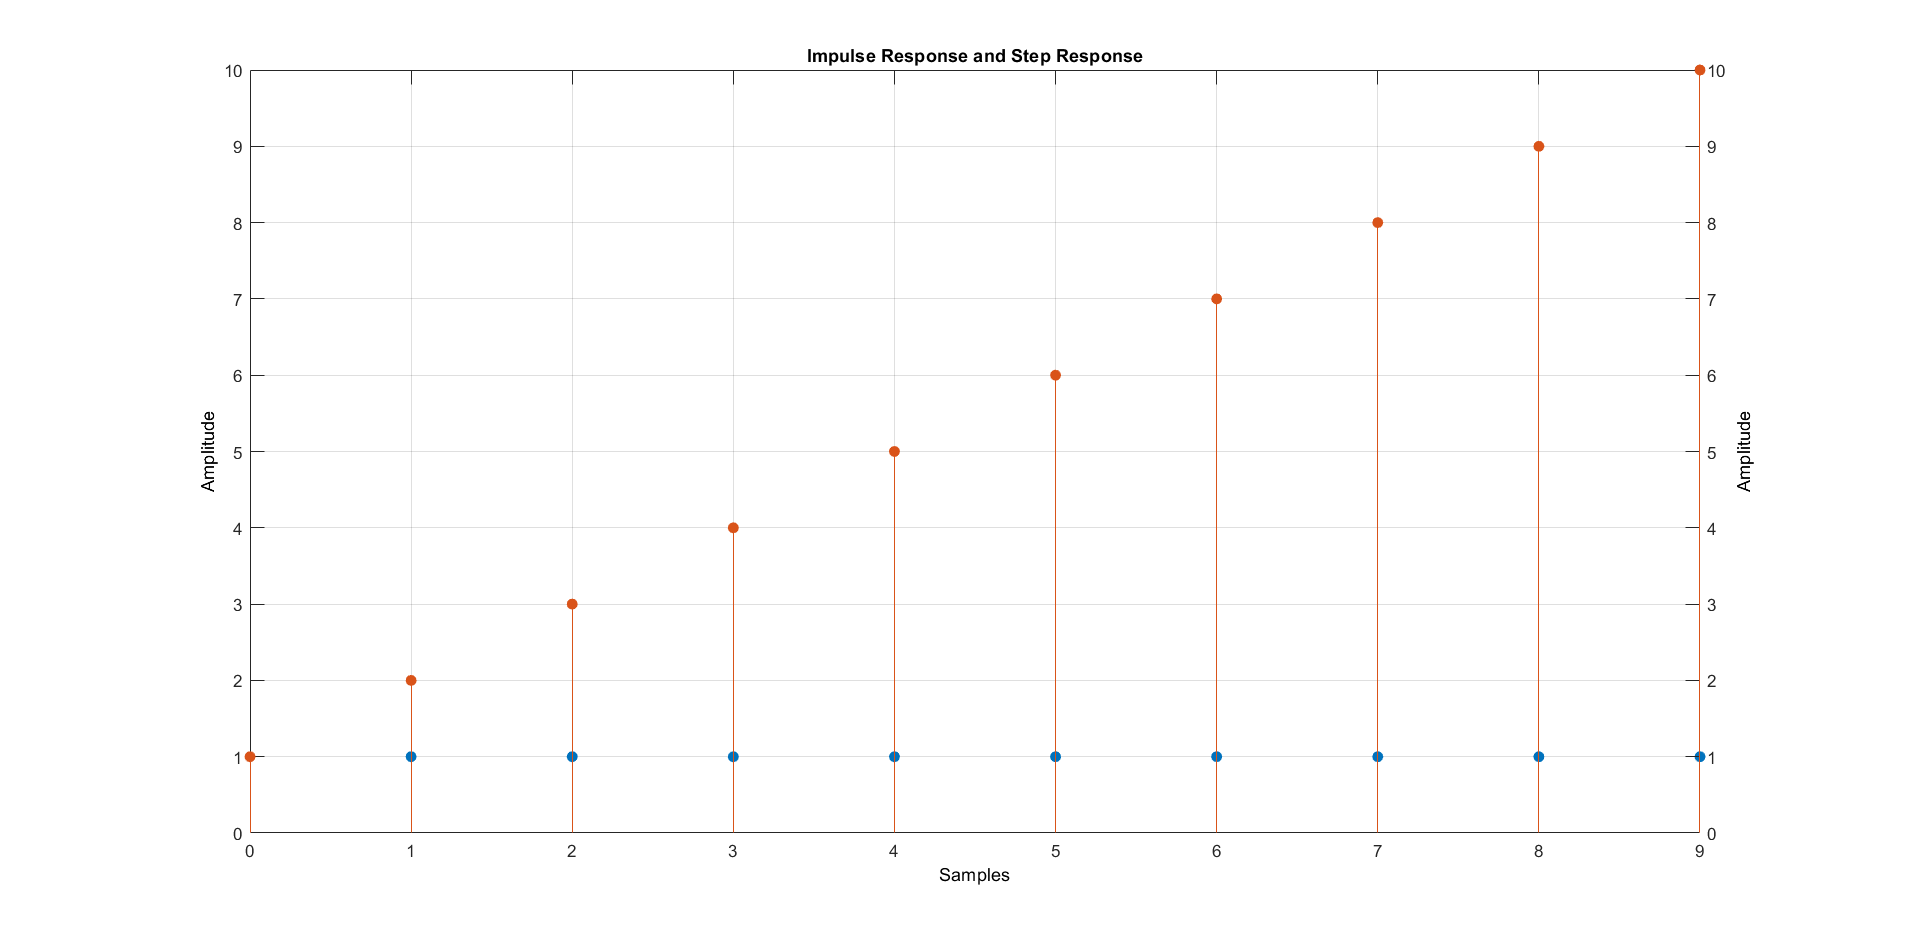
\includegraphics[width=1.0\linewidth]{res/2_7_ideal.png}
		\caption{Осциллограммы импульсной и переходной реакции}
	\end{figure}
	
	\begin{figure}[H]
		\centering
		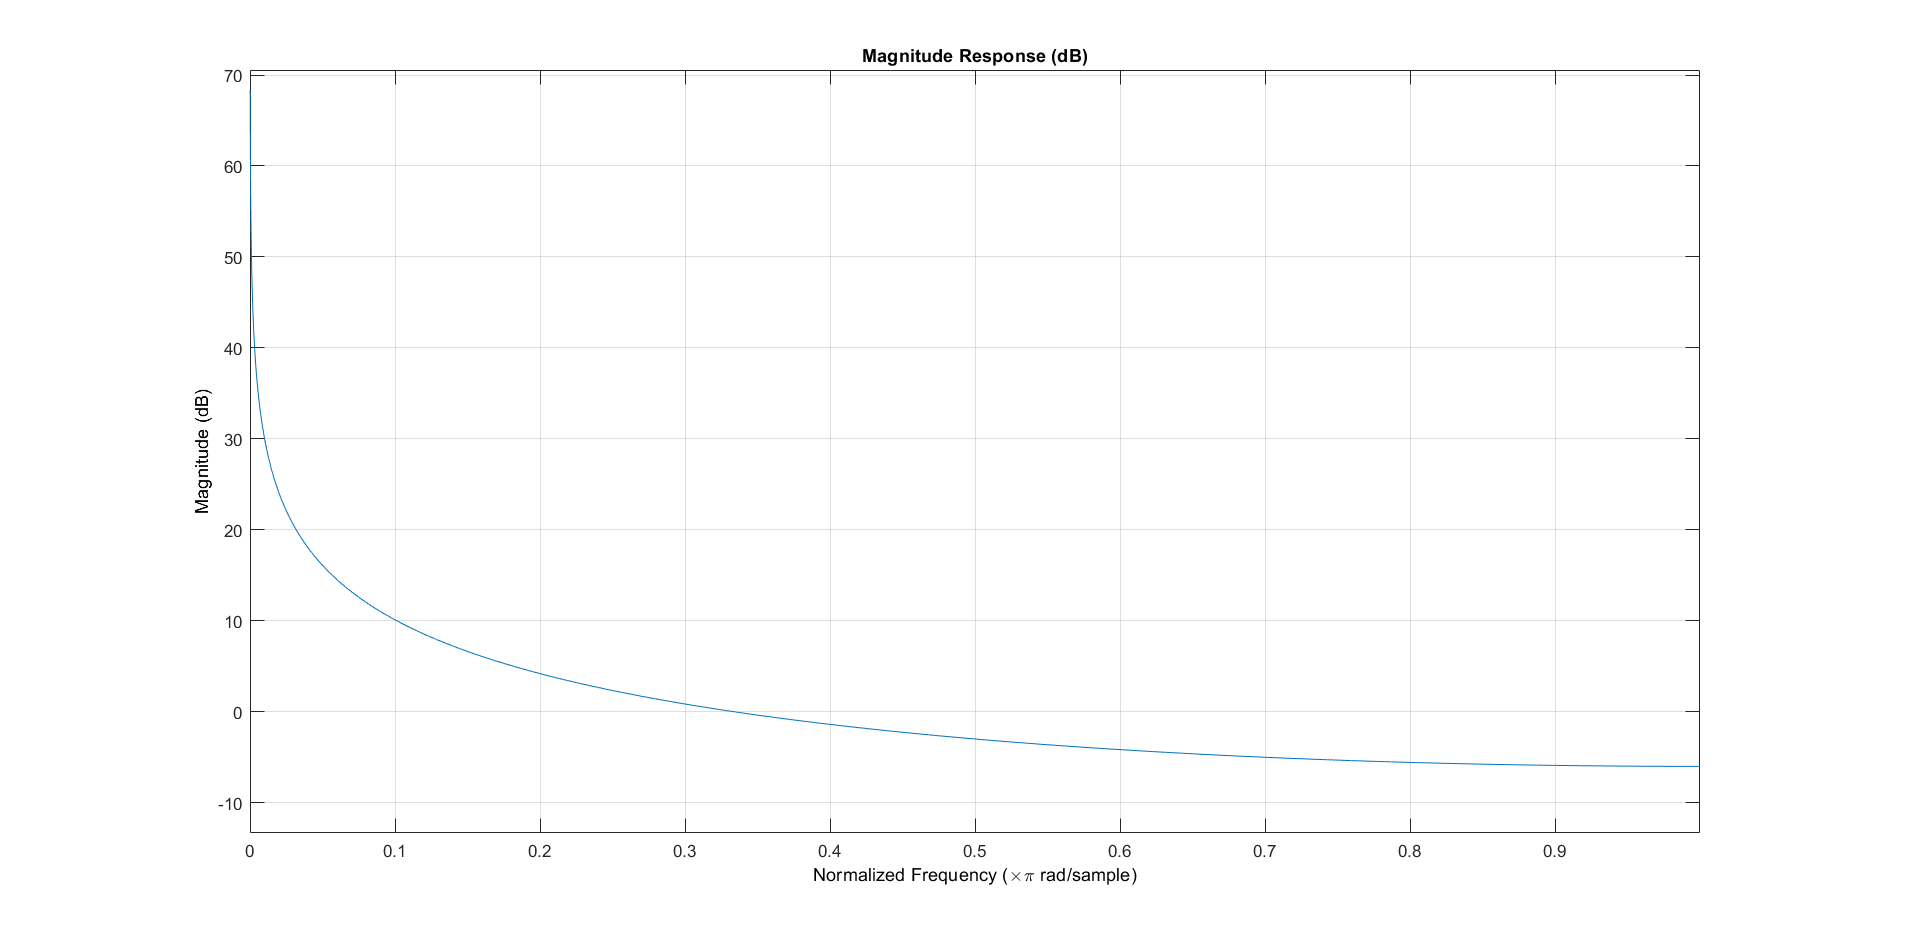
\includegraphics[width=1.0\linewidth]{res/2_7_idealach.png}
		\caption{Передаточная функция идеального интегратора}
	\end{figure}	
	
	Реализуем дифференцирующее звено: $h = [1, -1]$, $g = [1, -0.7]$.
	
	\begin{figure}[H]
		\centering
		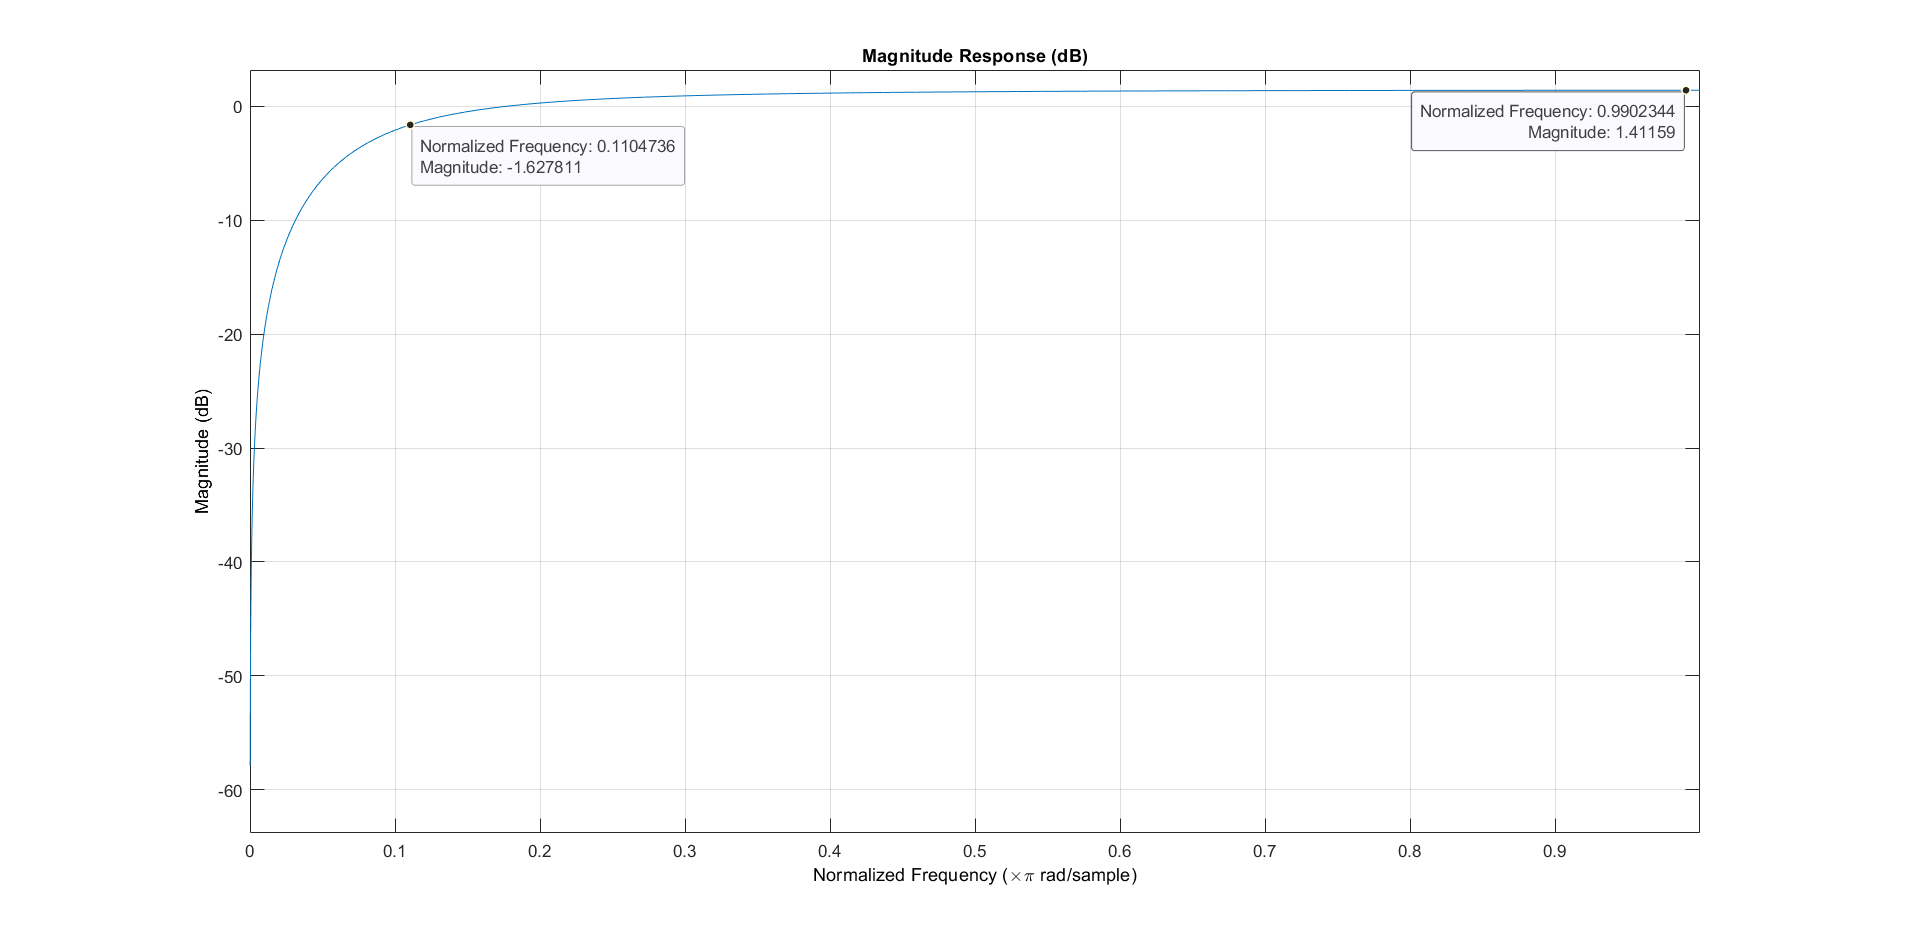
\includegraphics[width=1.0\linewidth]{res/2_8_ach.png}
		\caption{Передаточная функция дифференциатора}
	\end{figure}
	
	\begin{figure}[H]
		\centering
		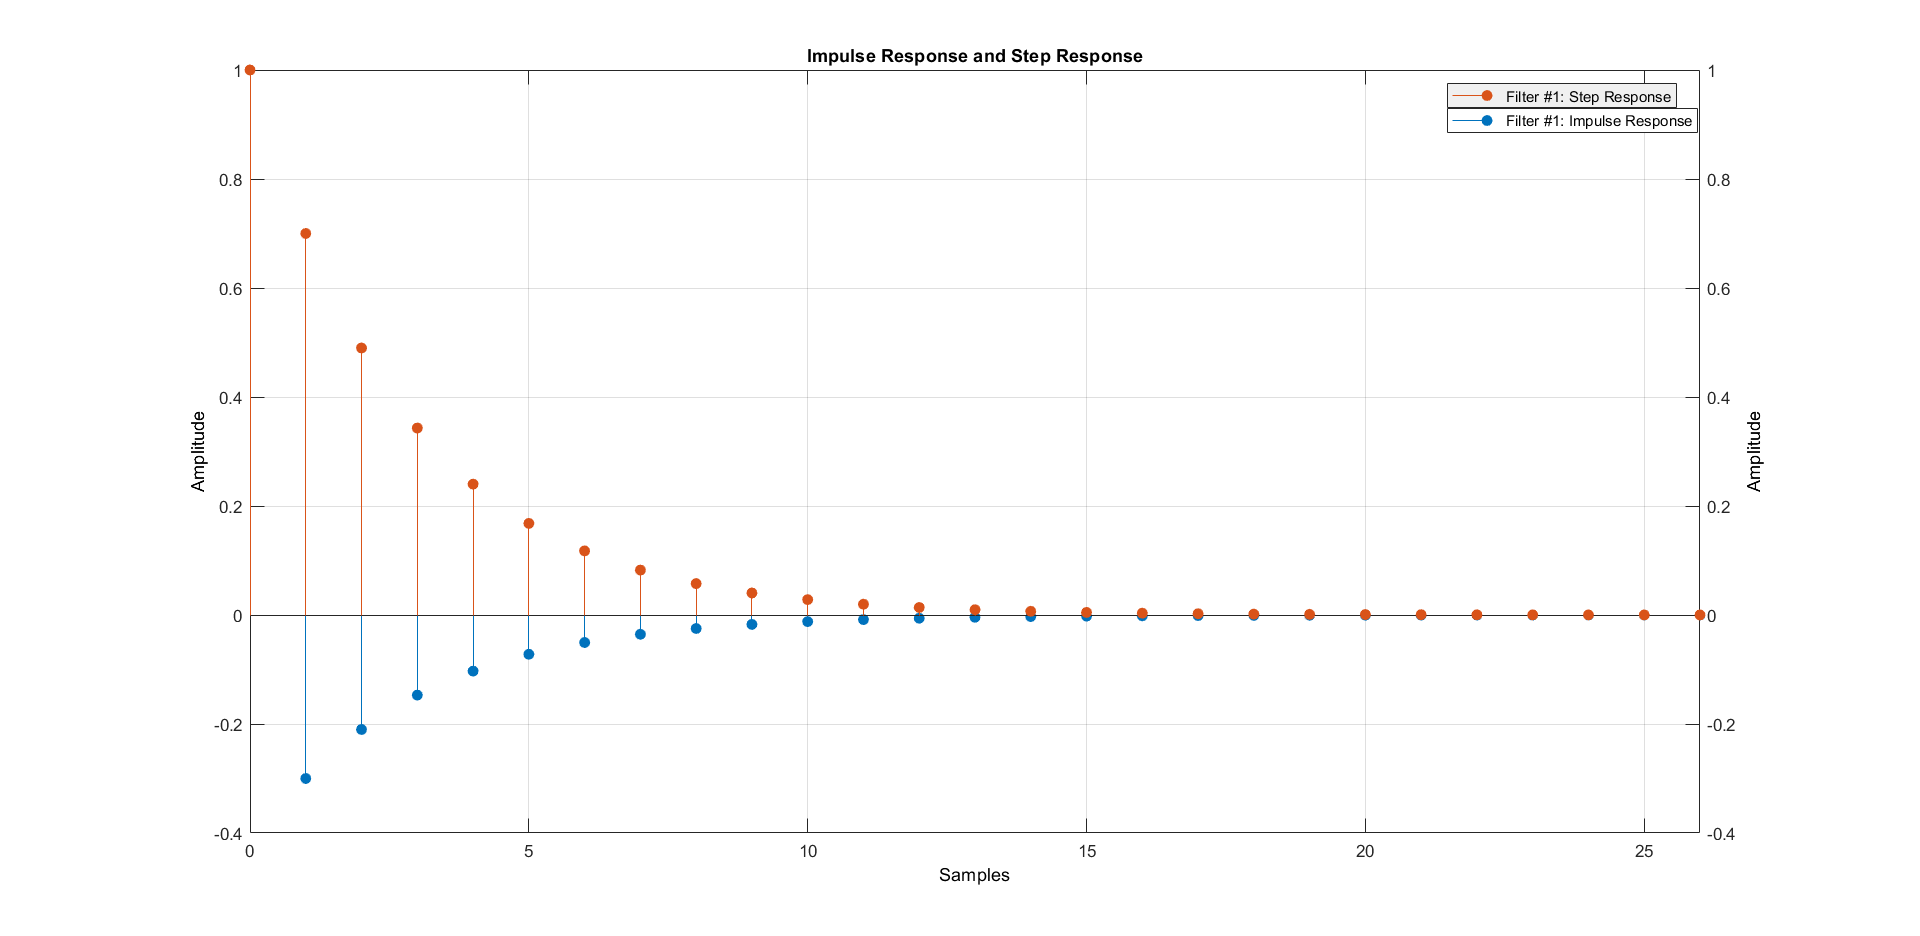
\includegraphics[width=1.0\linewidth]{res/2_8_impulse.png}
		\caption{Импульсная и переходная реакция дифференциатора}
	\end{figure}	
	
	Формула $f_0 = \frac{1}{2 \pi \tau}$ выполняется.
	
	Рассмотрим также идеальный дифференциатор с $\mu = 0$:
	
	\begin{figure}[H]
		\centering
		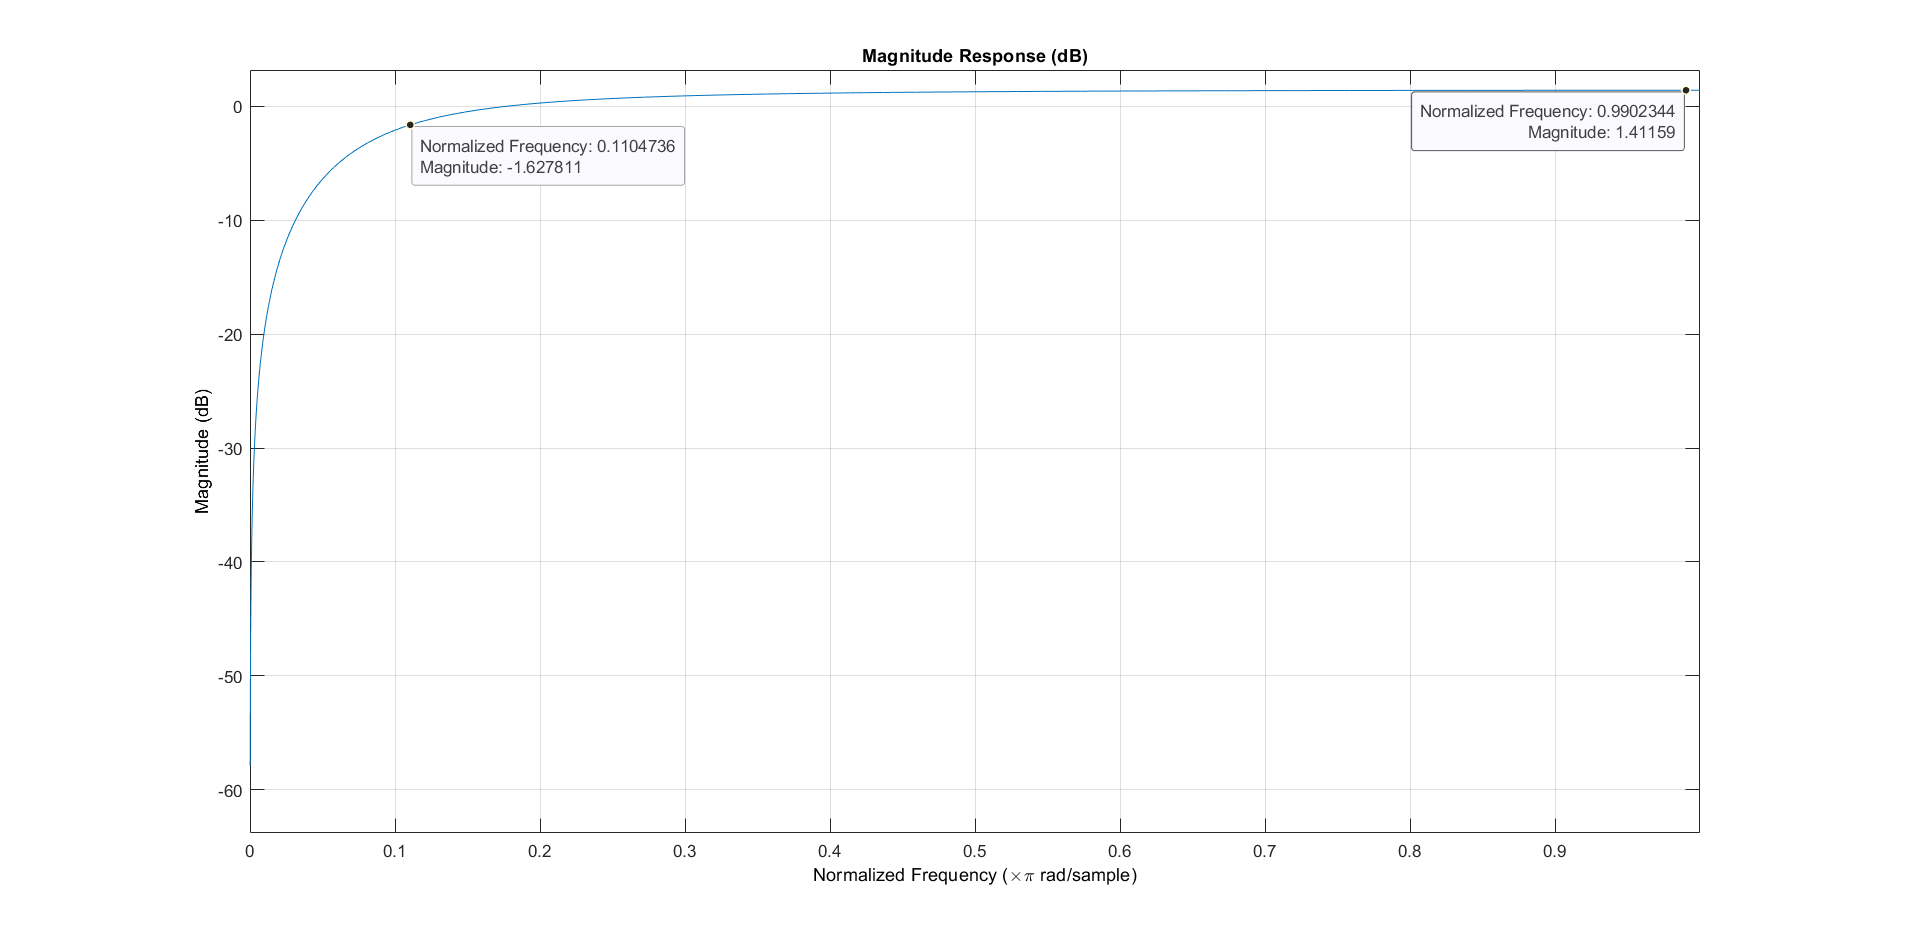
\includegraphics[width=1.0\linewidth]{res/2_8_ach.png}
		\caption{Передаточная функция идеального дифференциатора}
	\end{figure}
	
	\begin{figure}[H]
		\centering
		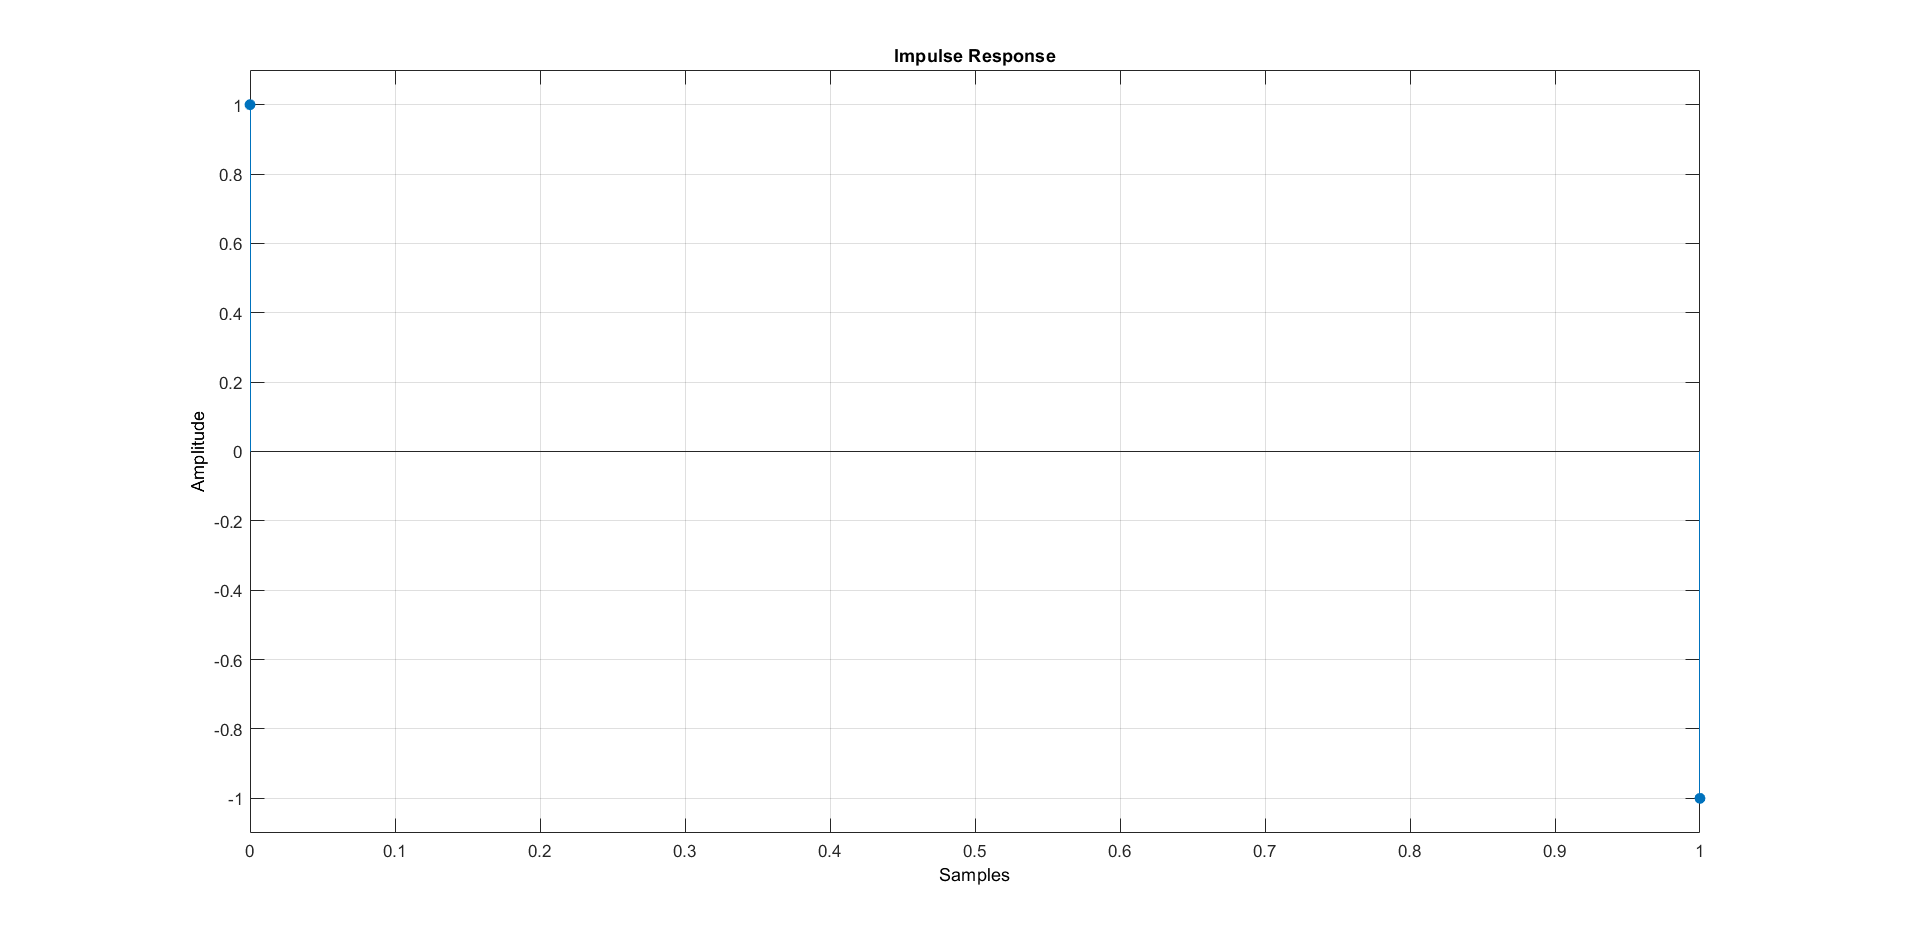
\includegraphics[width=1.0\linewidth]{res/2_8_idealimpulse.png}
		\caption{Импульсная реакция дифференциатора}
	\end{figure}	
	
	Переходной реакцией является $\delta$-функция.
	\begin{figure}[H]
		\centering
		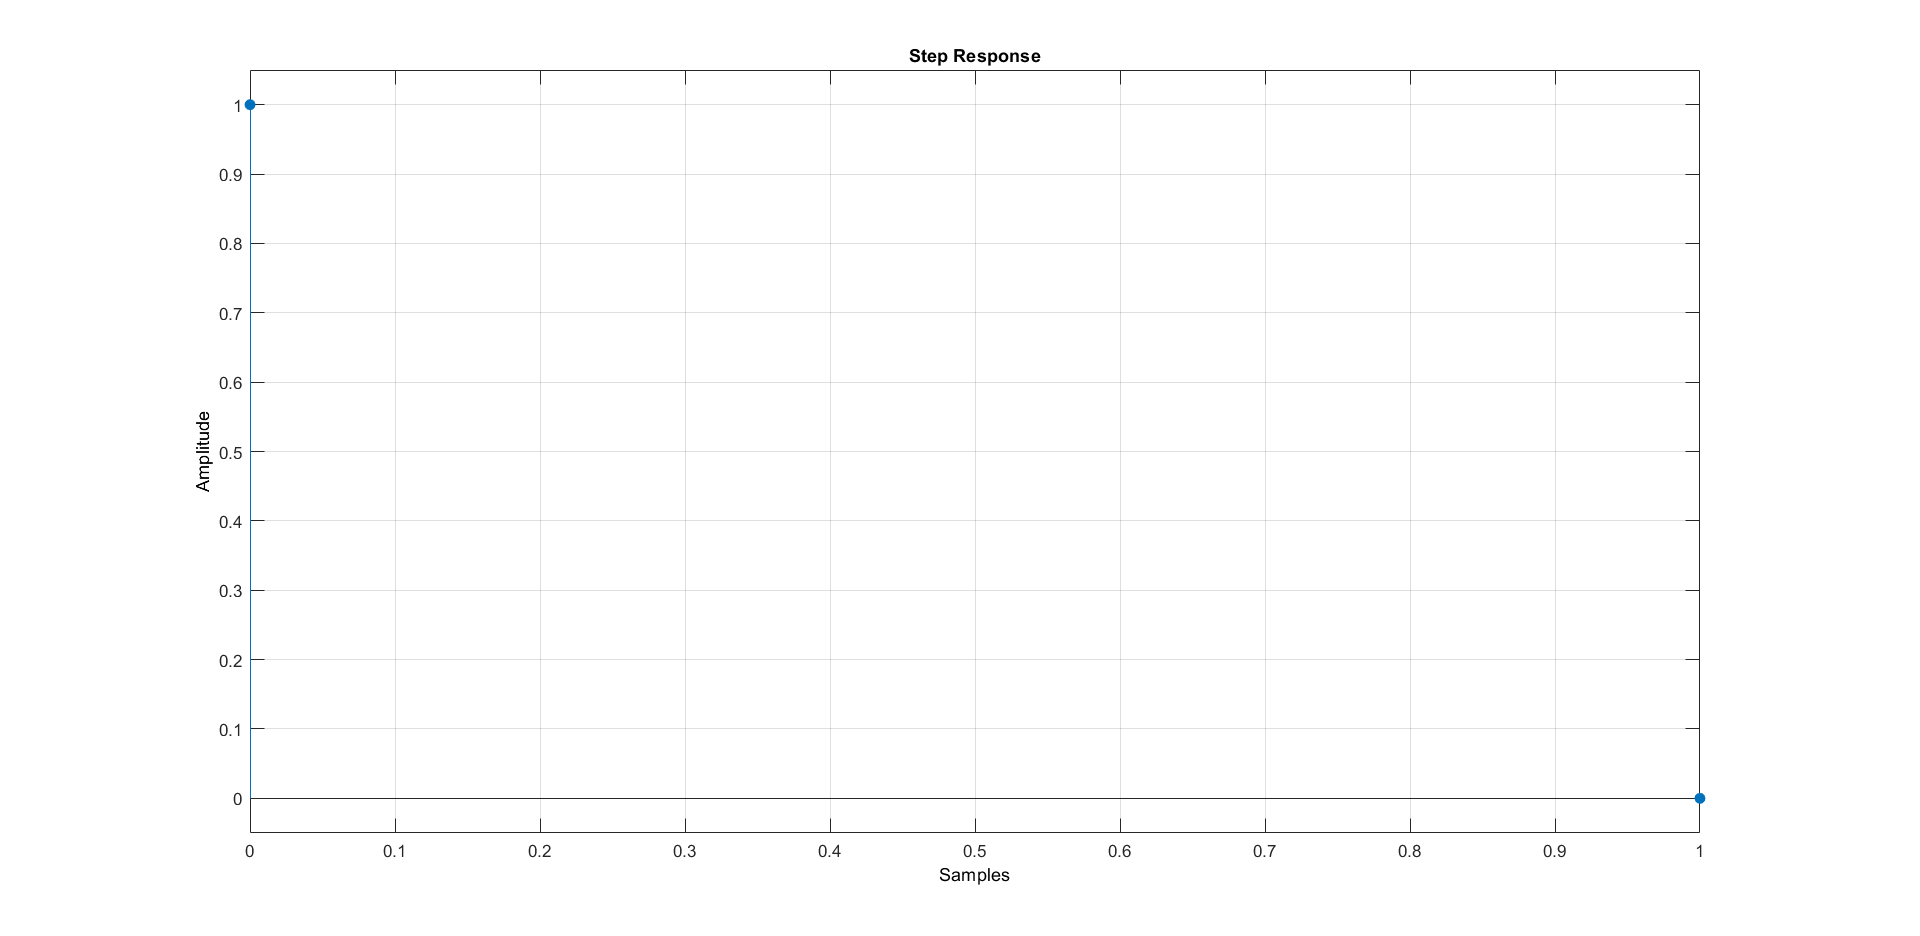
\includegraphics[width=1.0\linewidth]{res/2_8_idealstep.png}
		\caption{Переходная реакция дифференциатора}
	\end{figure}	
	
	Реализуем цифровой фазовращатель:
	$$ H(x) = \frac{-\mu + x}{1 - \mu x} \Leftrightarrow H(z) = \frac{1 - \mu z}{z - \mu}.$$
	$h = [-0.7, 1]$, $g = [1, -0.7]$.
	\begin{figure}[H]
		\centering
		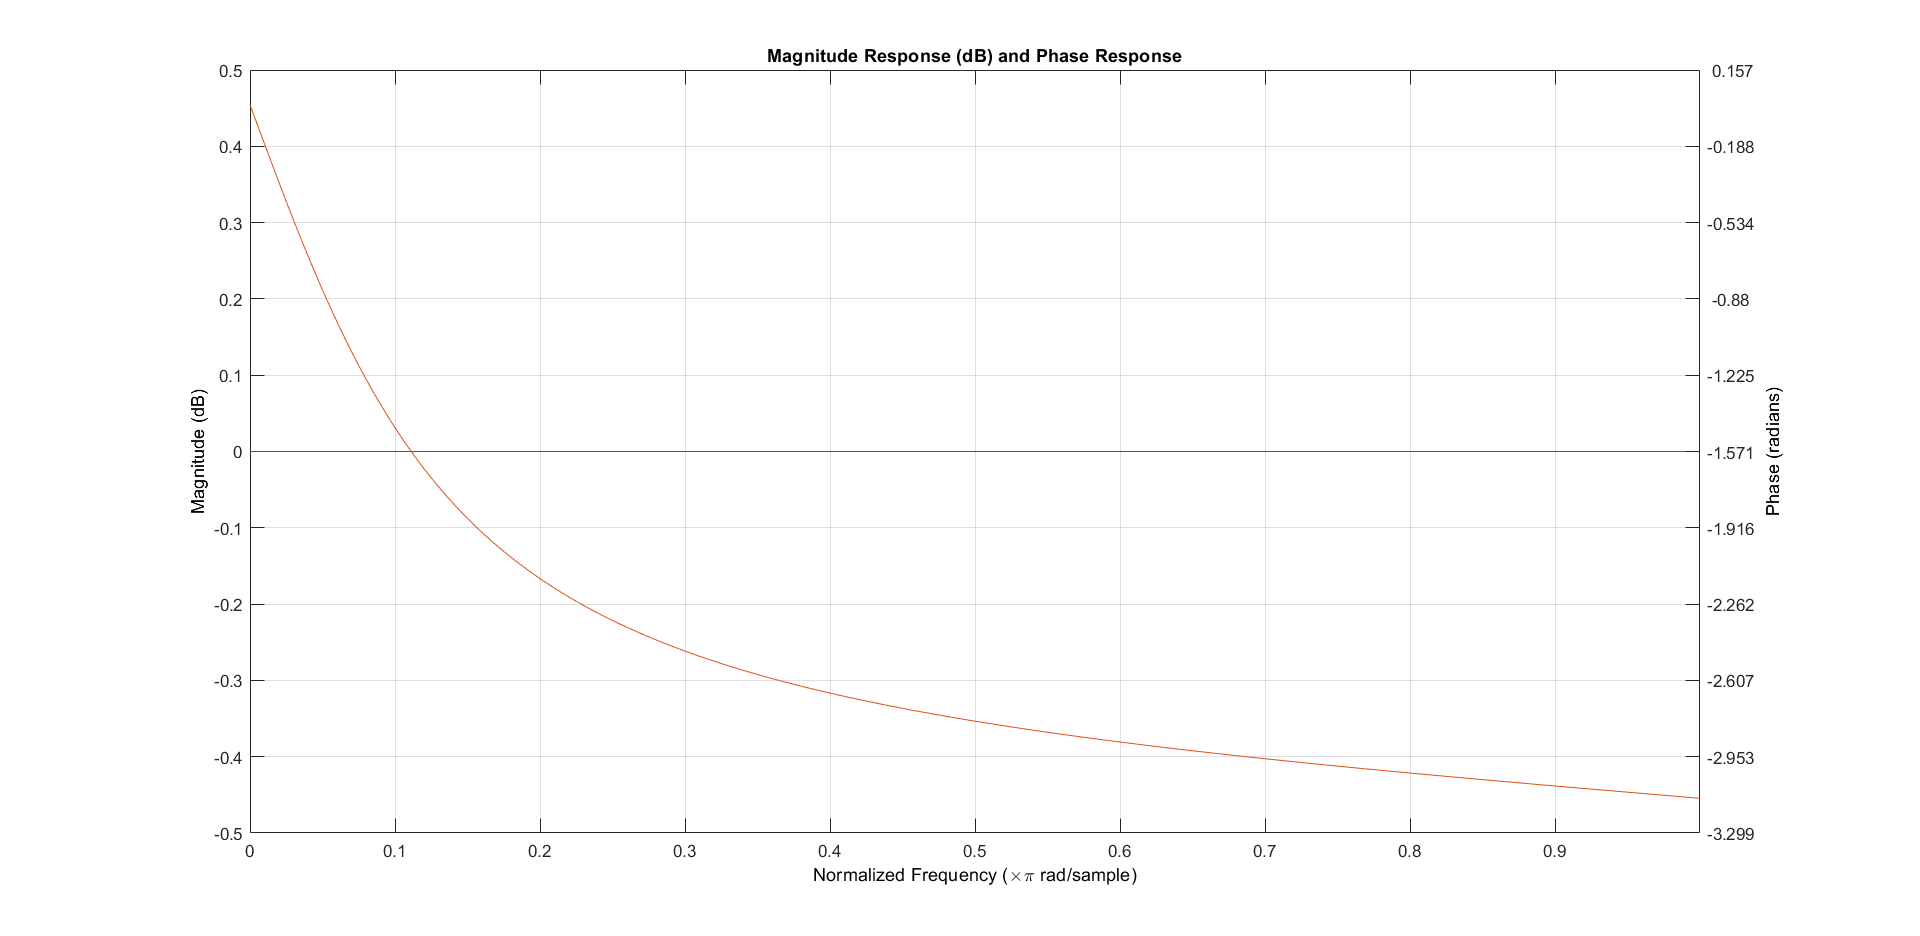
\includegraphics[width=1.0\linewidth]{res/2_9_phaseshifter.png}
		\caption{Переходная реакция фазовращателя}
	\end{figure}
	
	\subsection*{3. Звенья второго порядка}
	Реализуем полосовой фильтр второго порядка:
	$$ H_{\text{ПФ}} = \frac{1 - x^2}{1 - 2 r_{\mu} \cos( \varphi_\mu x) + r_\mu^2 x^2}\qquad r_\mu = 0.9, \; \varphi_\mu = \pi / 4. $$
	$$h = [1, 0, -1], \; g = [1, -0.9 \cdot \sqrt{2}, -0.9^2].$$
	\begin{figure}[H]
		\centering
		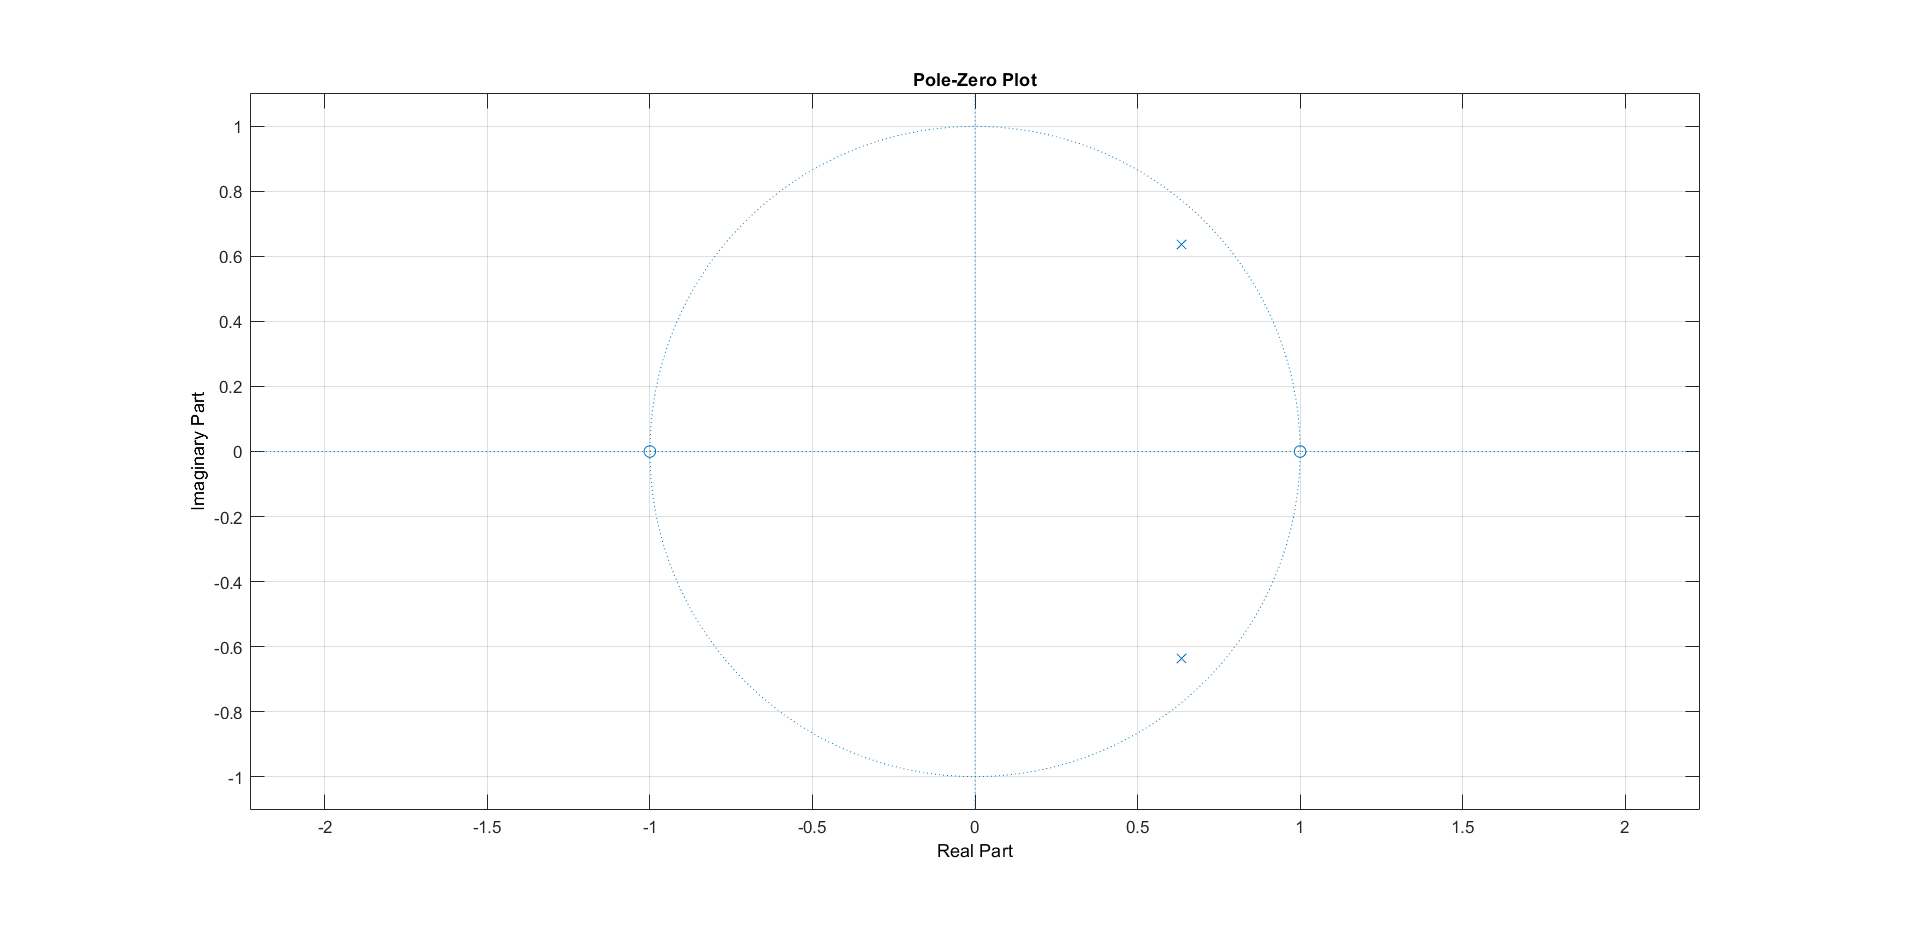
\includegraphics[width=1.0\linewidth]{res/3_1_bandpass_poles.png}
		\caption{Карта полосового фильтра}
	\end{figure}
	
	\begin{figure}[H]
		\centering
		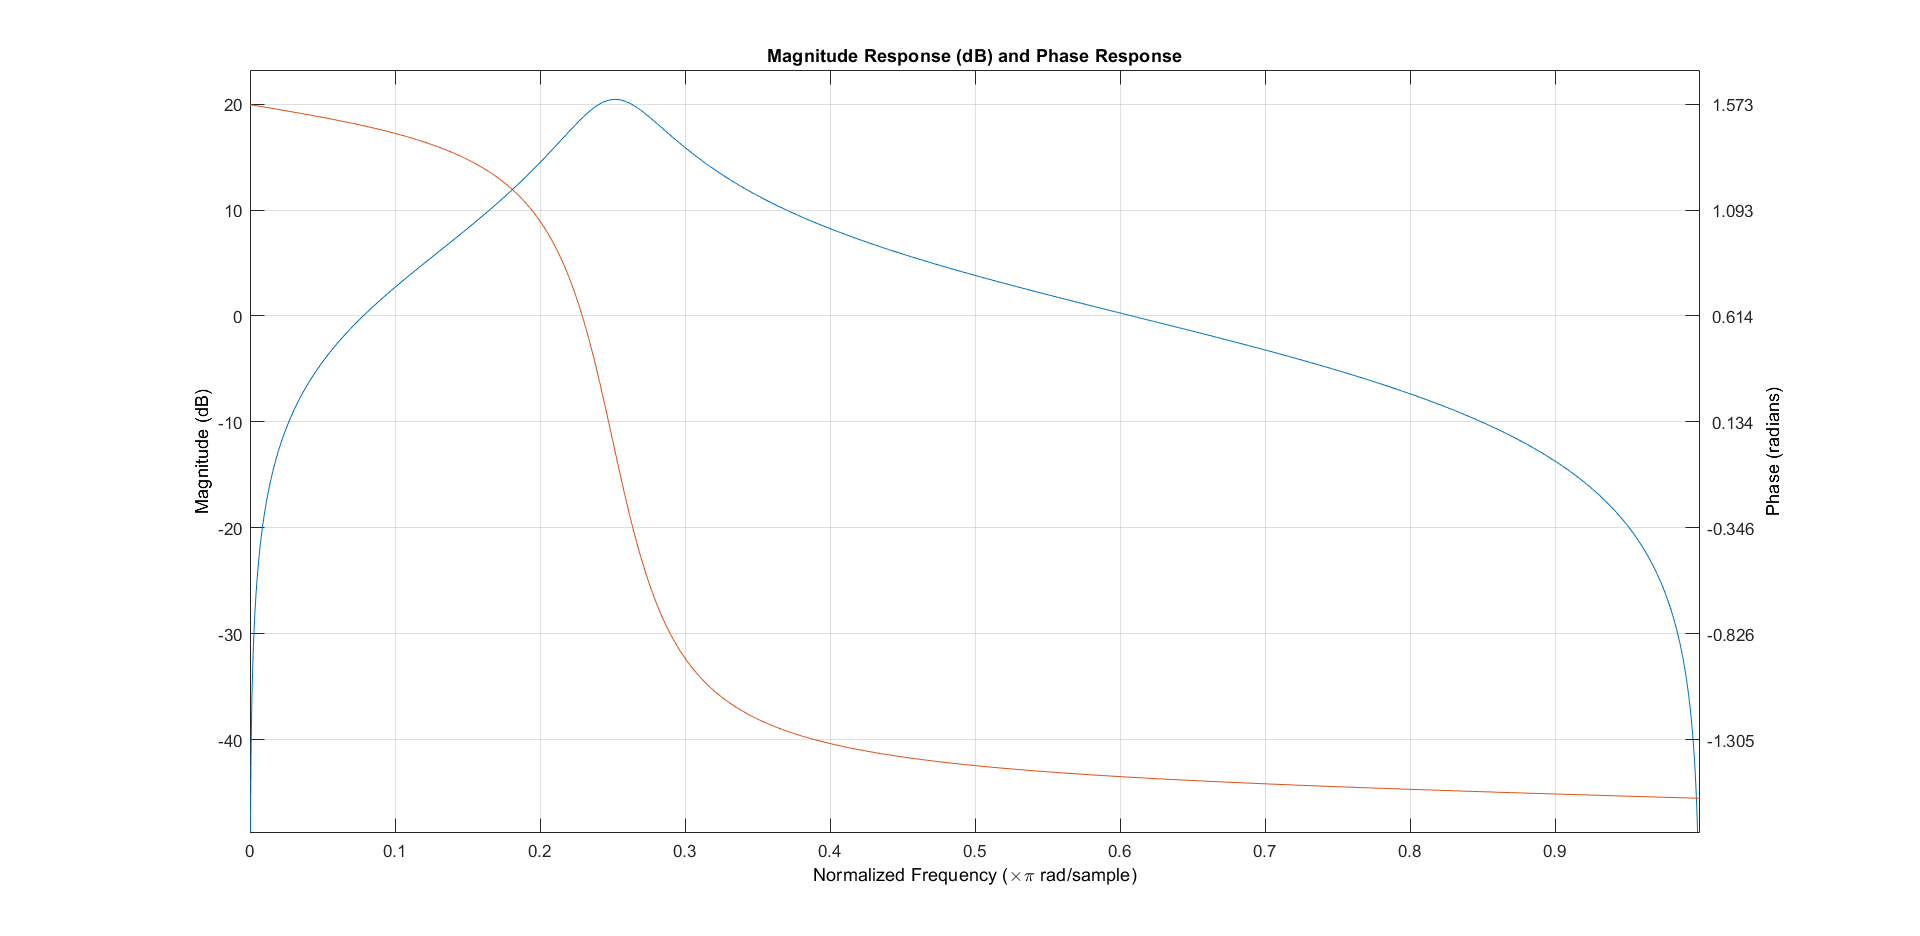
\includegraphics[width=1.0\linewidth]{res/3_1_bandpass.png}
		\caption{Частотные характеристики фильтра}
	\end{figure}
	
	$$ f_0 = 0.126 \qquad \Delta f = 0.035 \qquad 20 \lg K = 20.5 \;dB \qquad Q = f_0 / \Delta f = 3.8$$
	
	\begin{figure}[H]
		\centering
		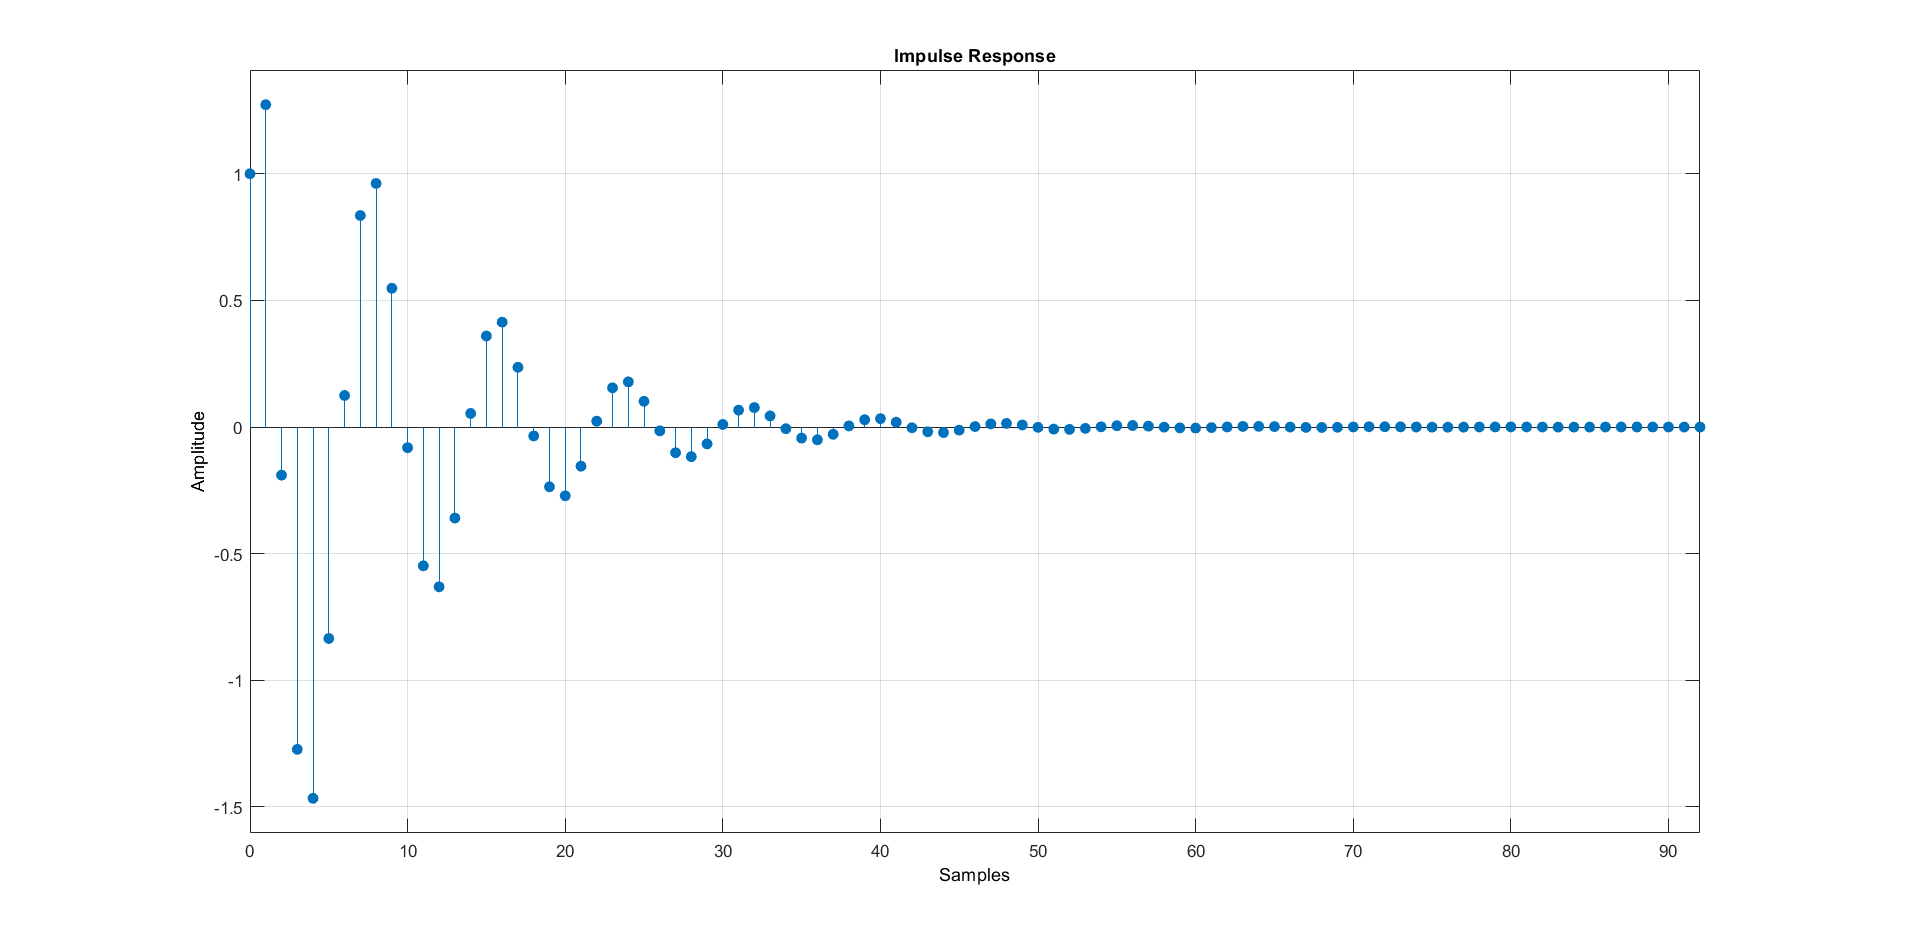
\includegraphics[width=1.0\linewidth]{res/3_1_impulse.png}
		\caption{Импульсная реакция}
	\end{figure}

	\begin{figure}[H]
		\centering
		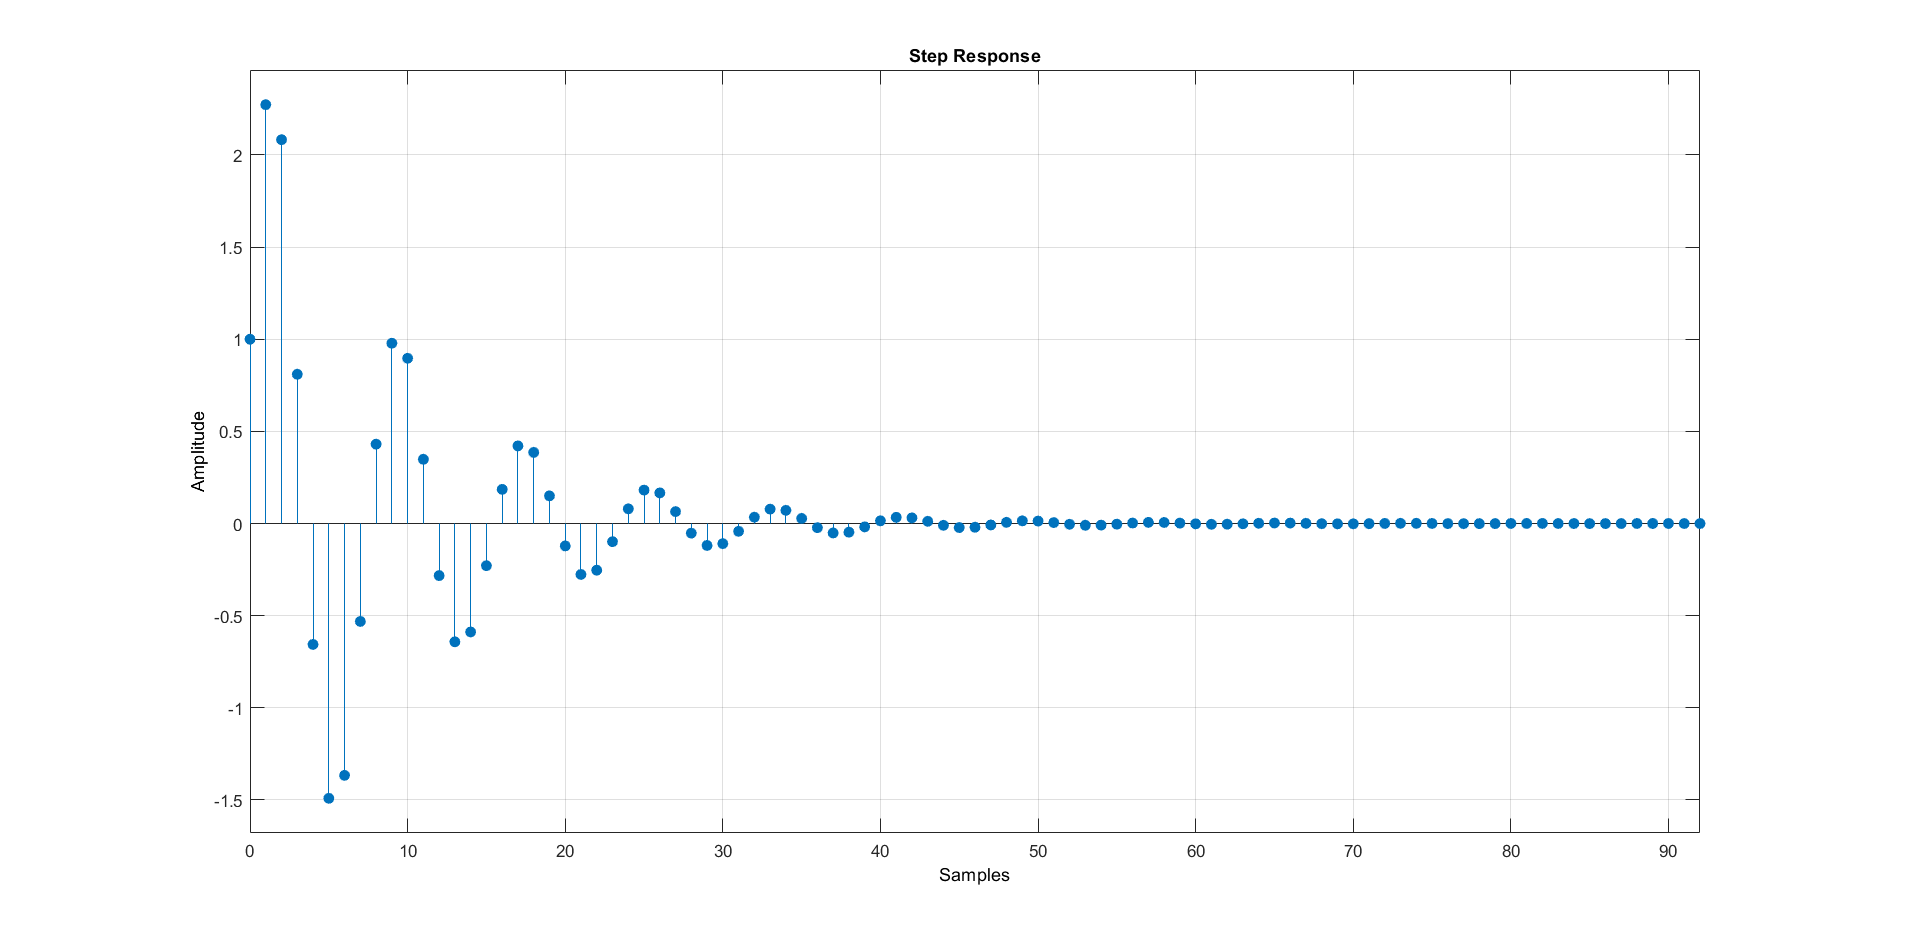
\includegraphics[width=1.0\linewidth]{res/3_1_step.png}
		\caption{Переходная реакция}
	\end{figure}

	Изучим зависимость фильтра от $r_\mu \rightarrow 1$. $r_\mu = 0.98$.
	
	\begin{figure}[H]
		\centering
		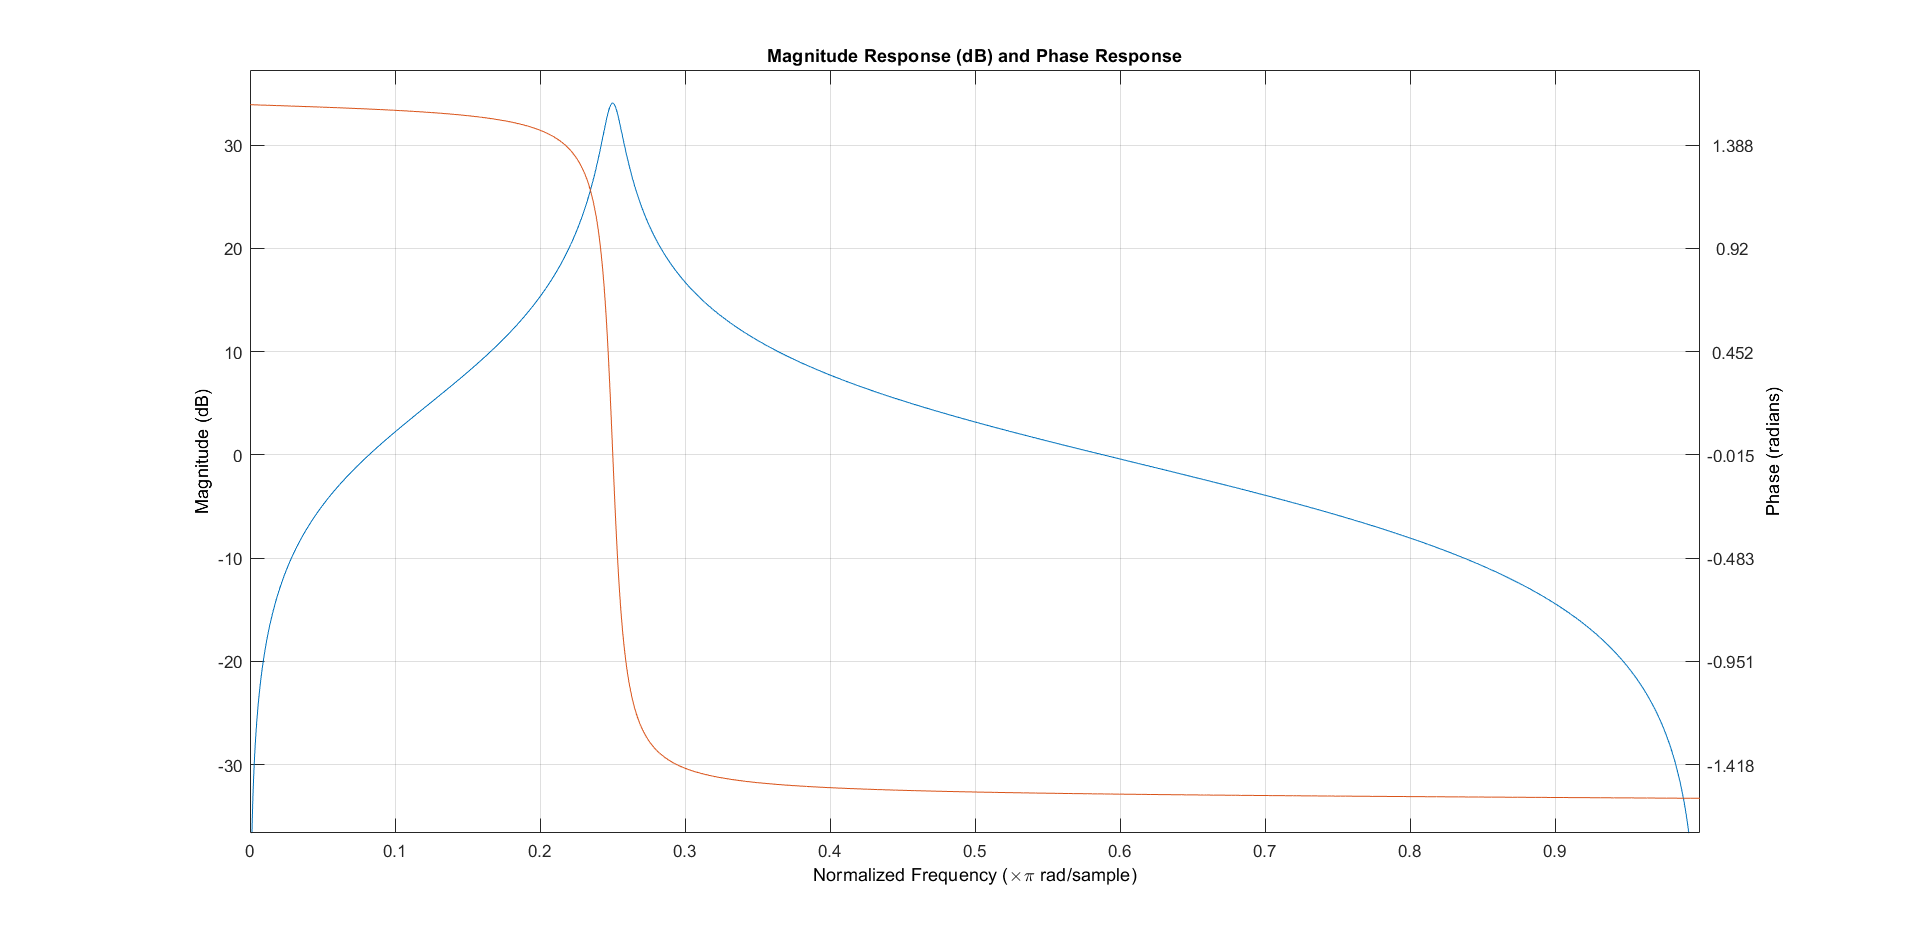
\includegraphics[width=1.0\linewidth]{res/3_2_bandpass_098.png}
		\caption{Частотные характеристики фильтра}
	\end{figure}
	
	Рассмотрим трансформации в ФНЧ, ФВЧ и чисто рекурсивные фильтры:

	\begin{figure}[H]
		\centering
		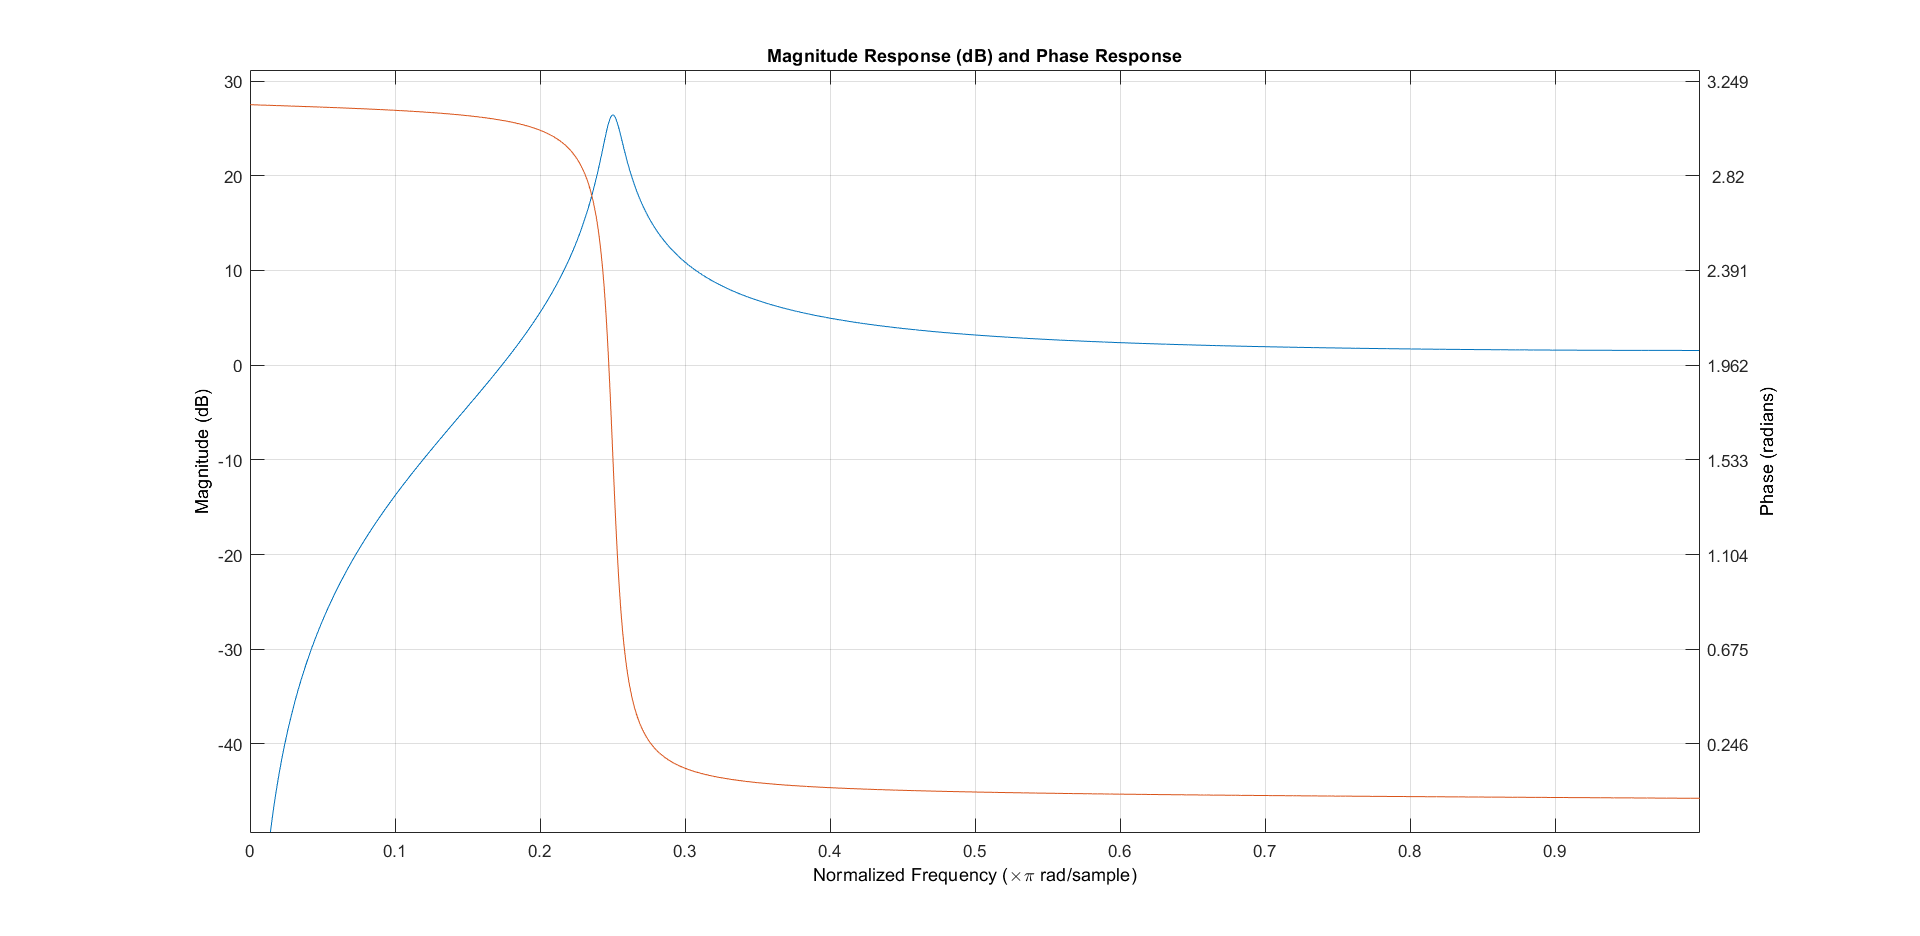
\includegraphics[width=1.0\linewidth]{res/3_2_highpass.png}
		\caption{Частотные характеристики ФВЧ}
	\end{figure}

	\begin{figure}[H]
		\centering
		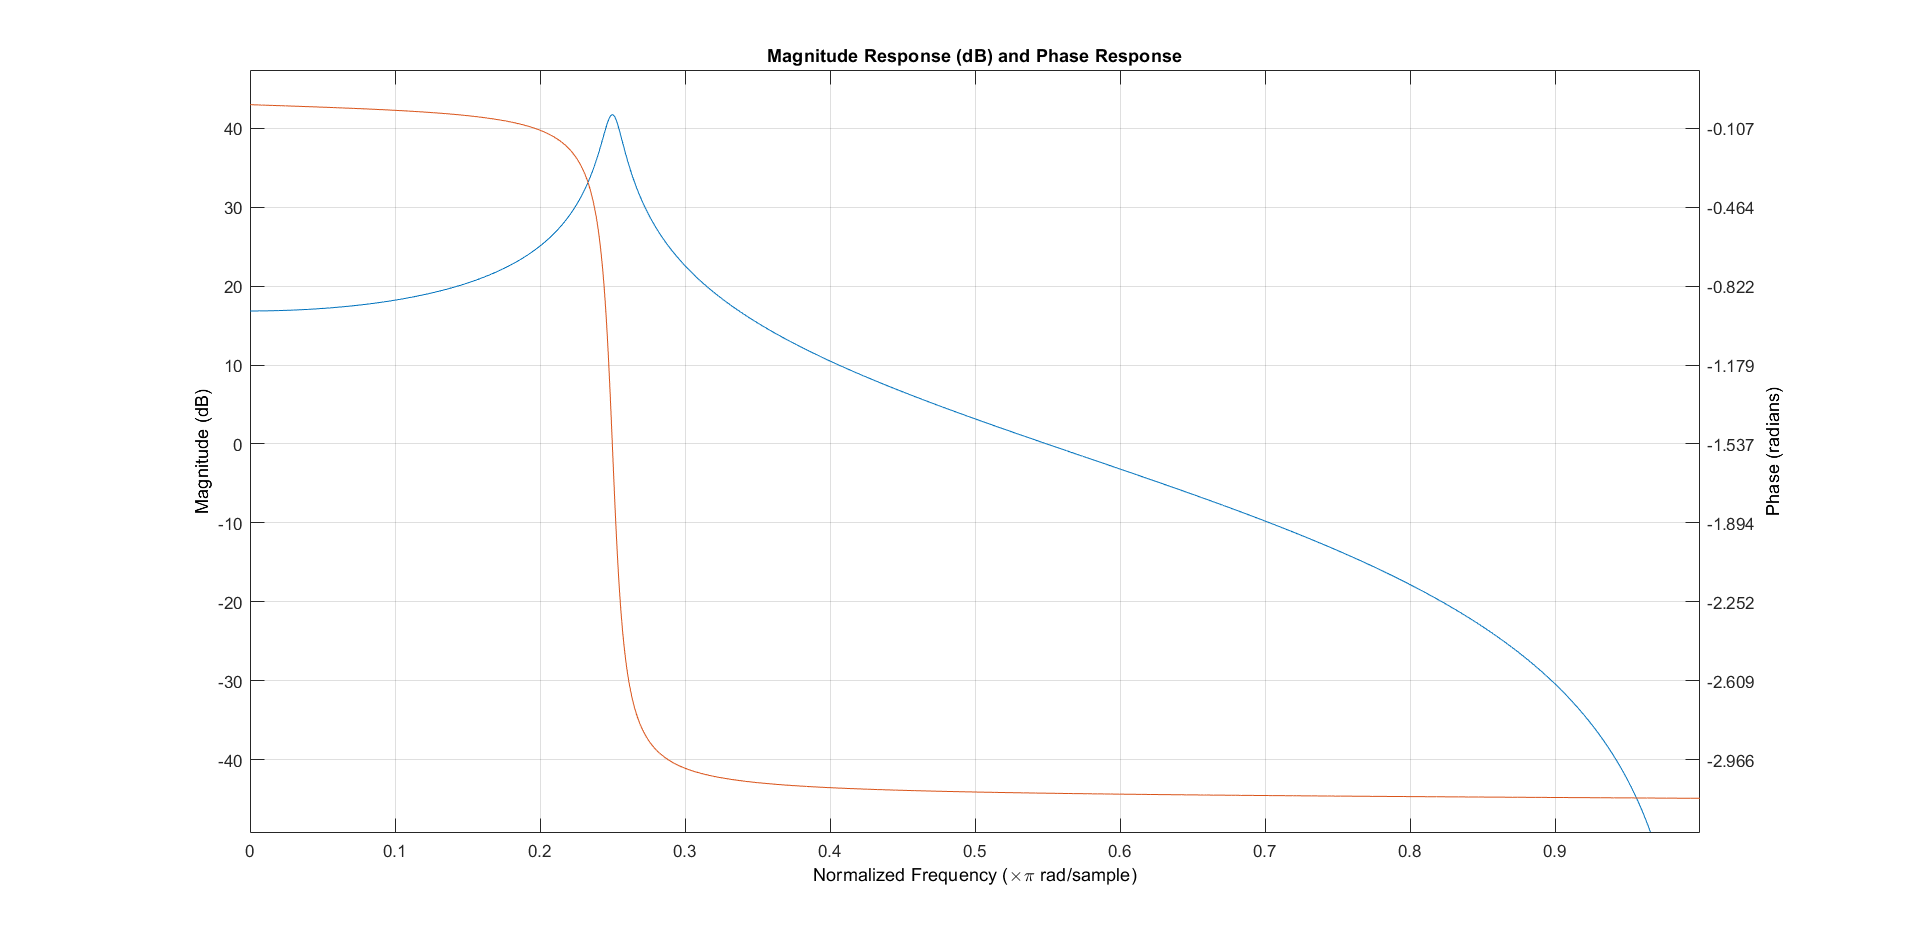
\includegraphics[width=1.0\linewidth]{res/3_2_lowpass.png}
		\caption{Частотные характеристики ФНЧ}
	\end{figure}
		
	\begin{figure}[H]
		\centering
		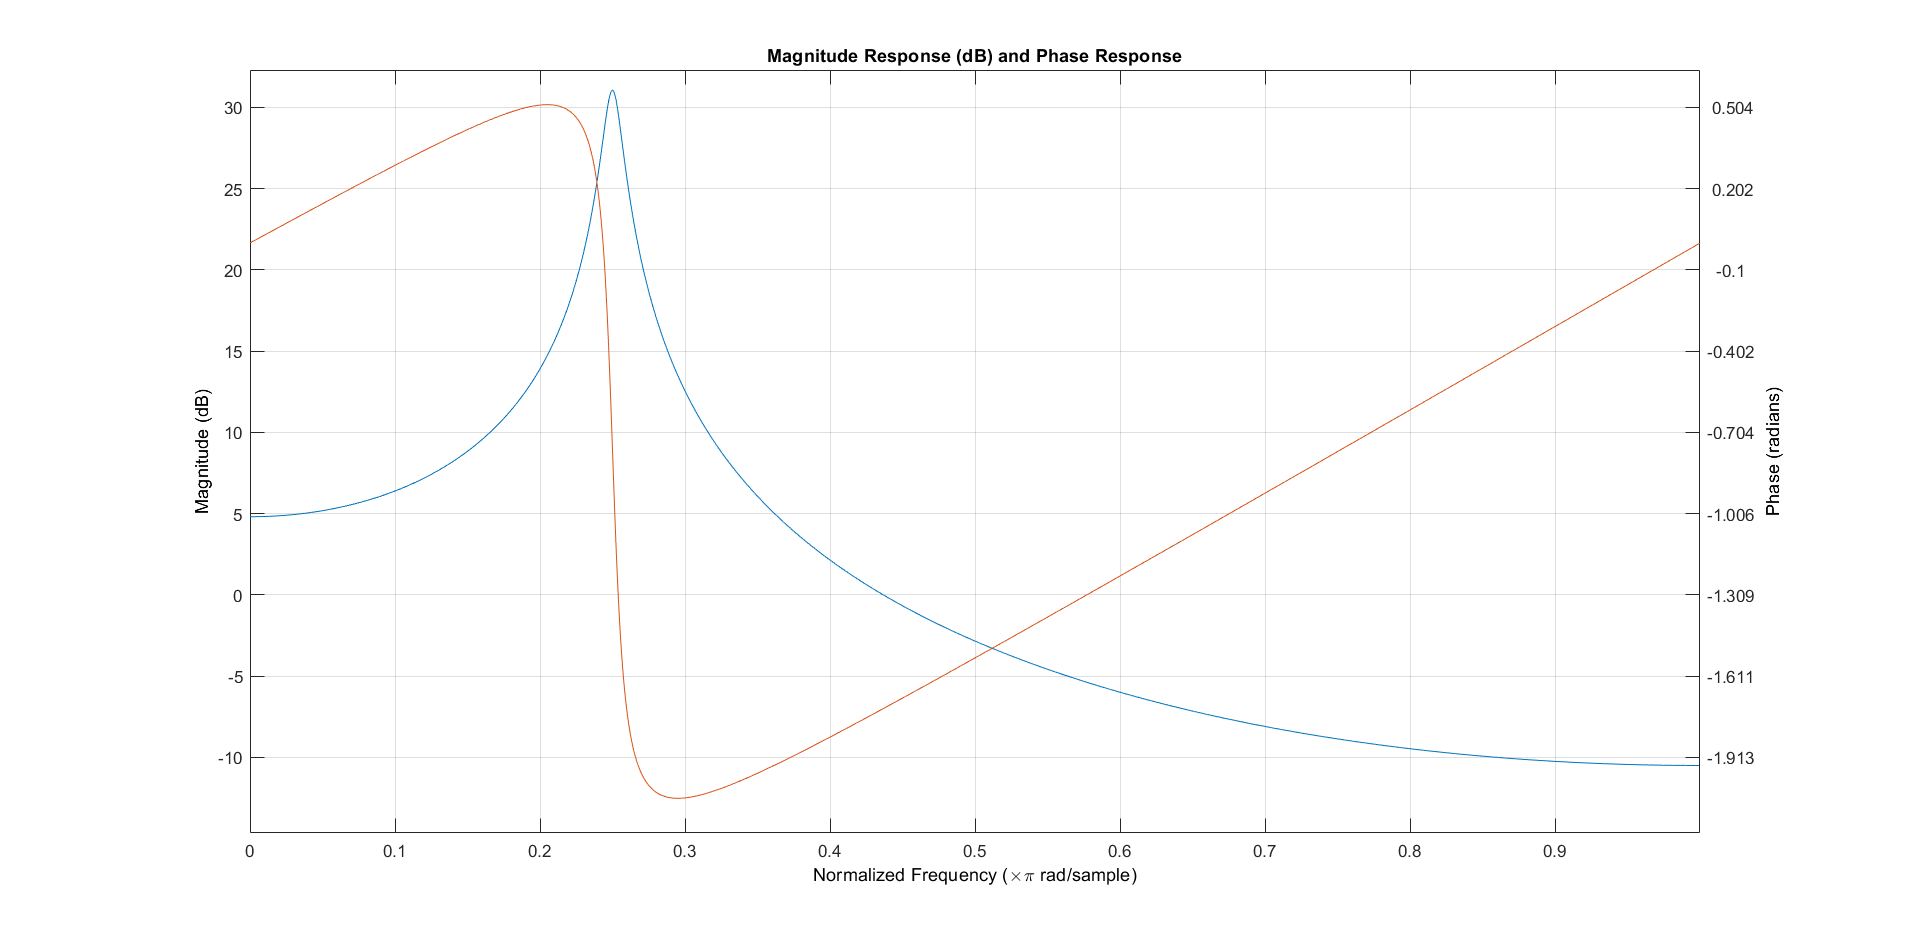
\includegraphics[width=1.0\linewidth]{res/3_2_allpoles.png}
		\caption{Частотные характеристики чисто рекурсивного (all poles)}
	\end{figure}

	Рассмотрим фильтр с парой сопряженных нулей:
	$$ H = 1 -2 r_\nu \cos( \varphi_\nu x) + r_\nu^2 x^2, \quad r_\nu = 0.9$$
	\begin{figure}[H]
		\centering
		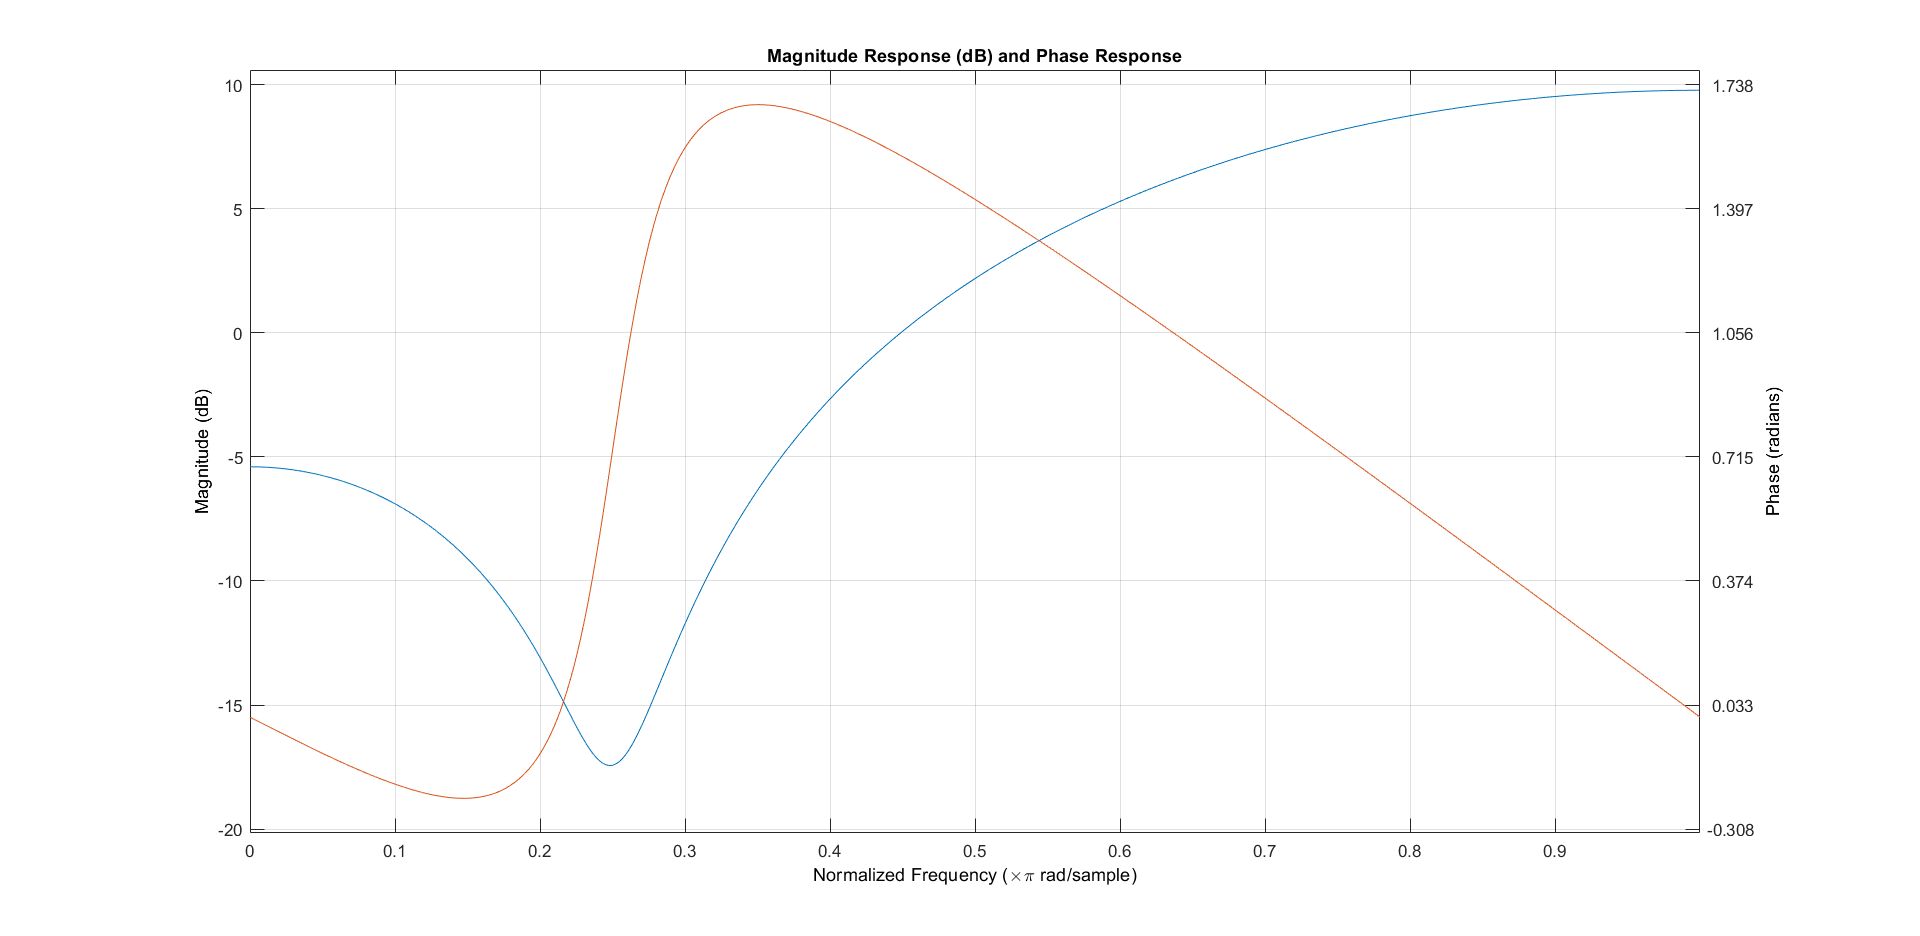
\includegraphics[width=1.0\linewidth]{res/3_3_09.png}
		\caption{Частотные характеристики фильтра с парой сопряженных нулей}
	\end{figure}
	
	Реализуем all pass фильтр с равномерной АЧХ:
	$$ r_\mu = 0.8 \qquad r_\nu = 1.25.$$
	\begin{figure}[H]
		\centering
		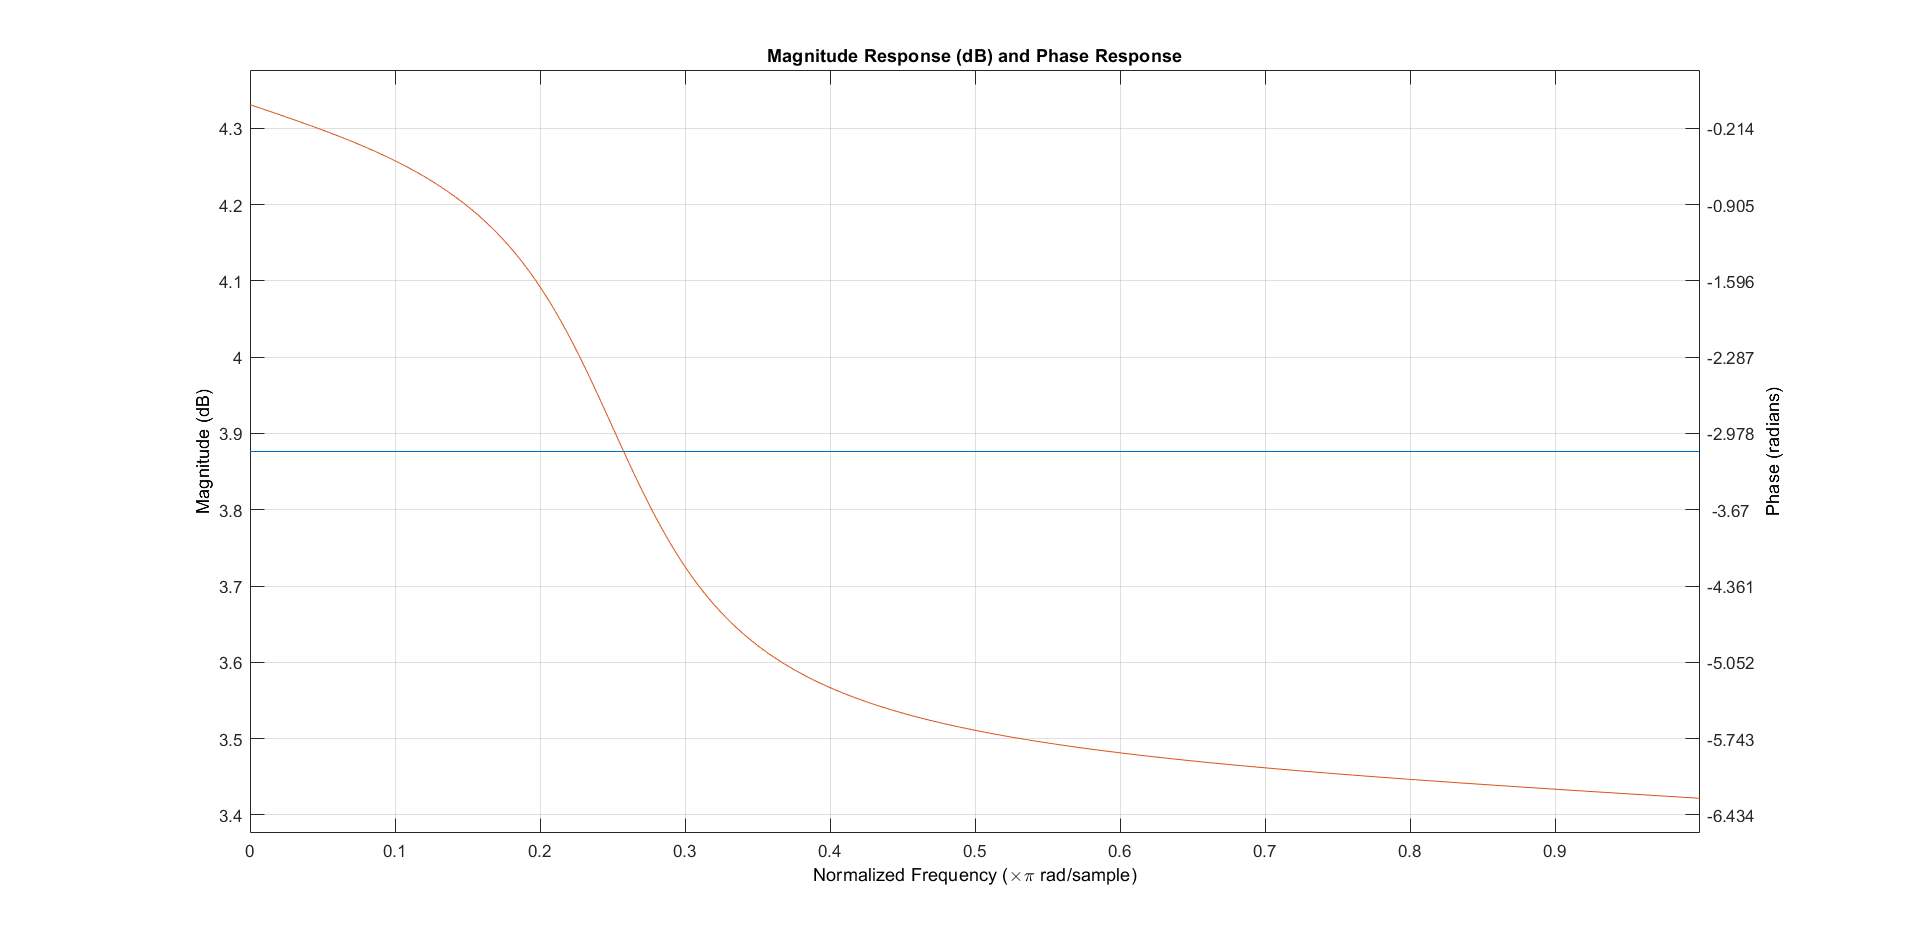
\includegraphics[width=1.0\linewidth]{res/3_4_allpass.png}
		\caption{Частотные характеристики фильтра}
	\end{figure}
	
	\subsection*{4. Нерекурсивные FIR фильтры}
	
	Все фильтры будут all zeros: $g = [1]$.
	
	Реализуем гребенчатый $N = 3$: $H(x) = 1 - x^3 \Rightarrow h = [1, 0, -1], g = [1]$.
	\begin{figure}[H]
		\centering
		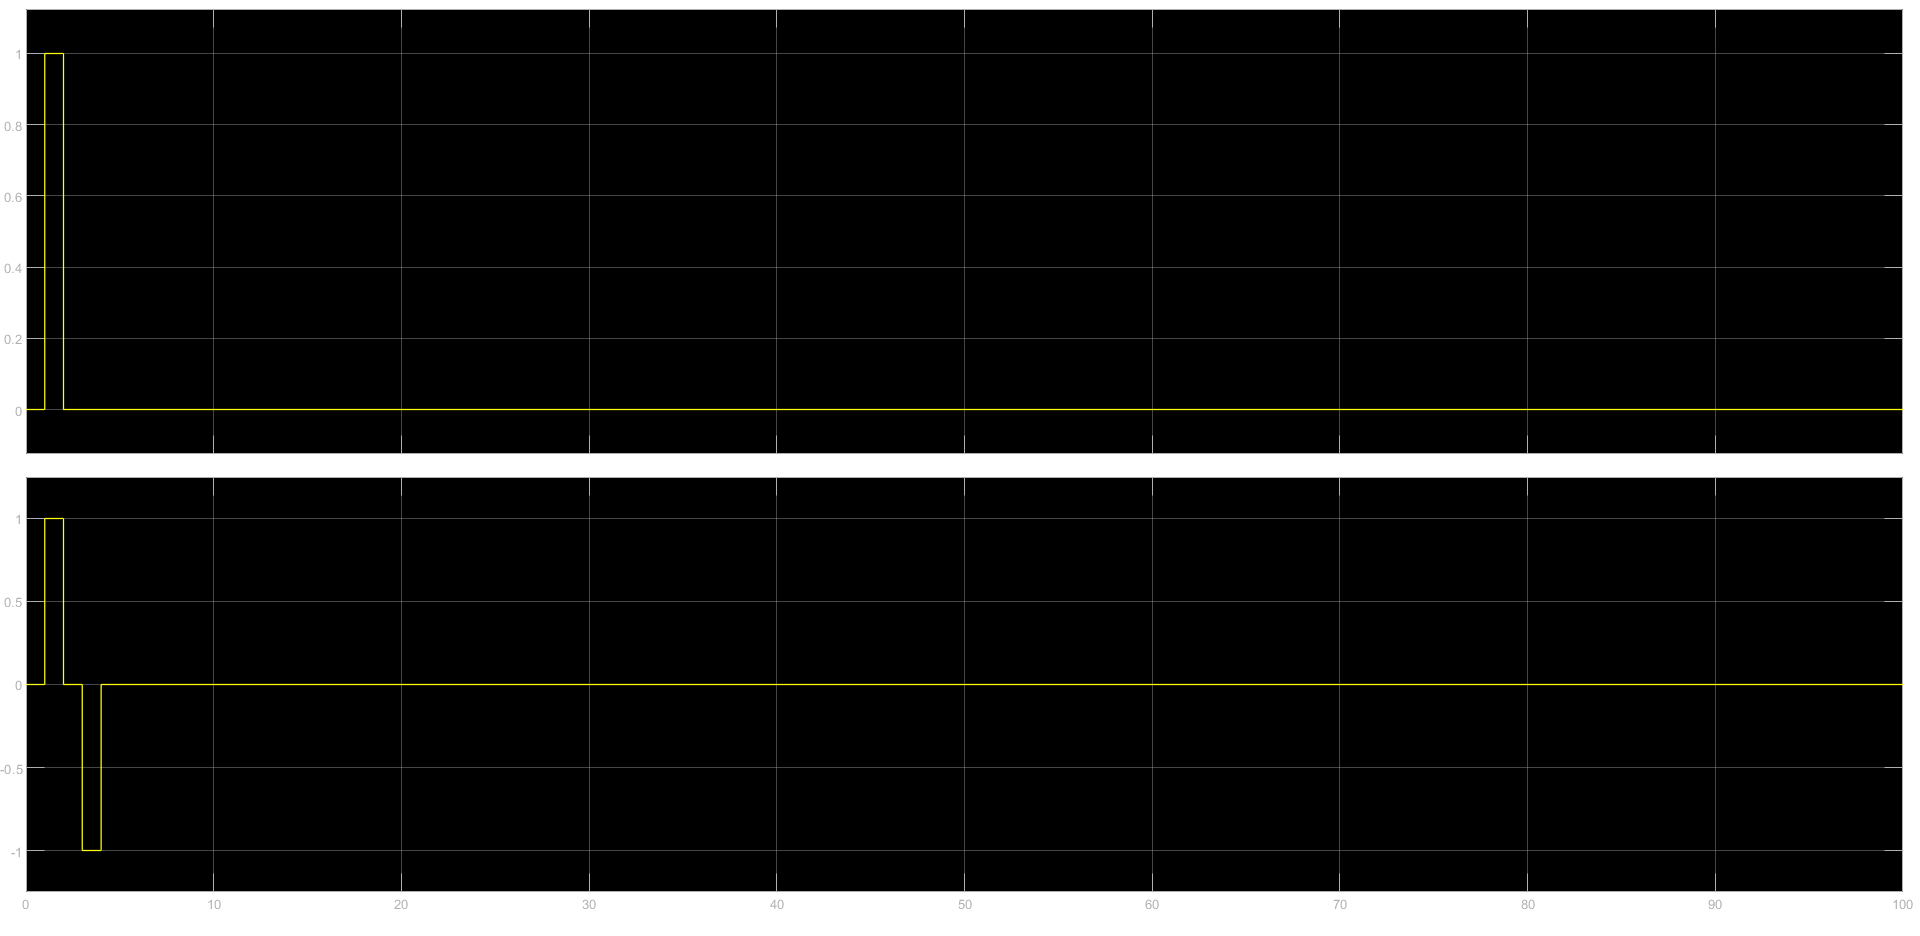
\includegraphics[width=1.0\linewidth]{res/4_1_time.png}
		\caption{Импульсная реакция фильтра}
	\end{figure}
		
	\begin{figure}[H]
		\centering
		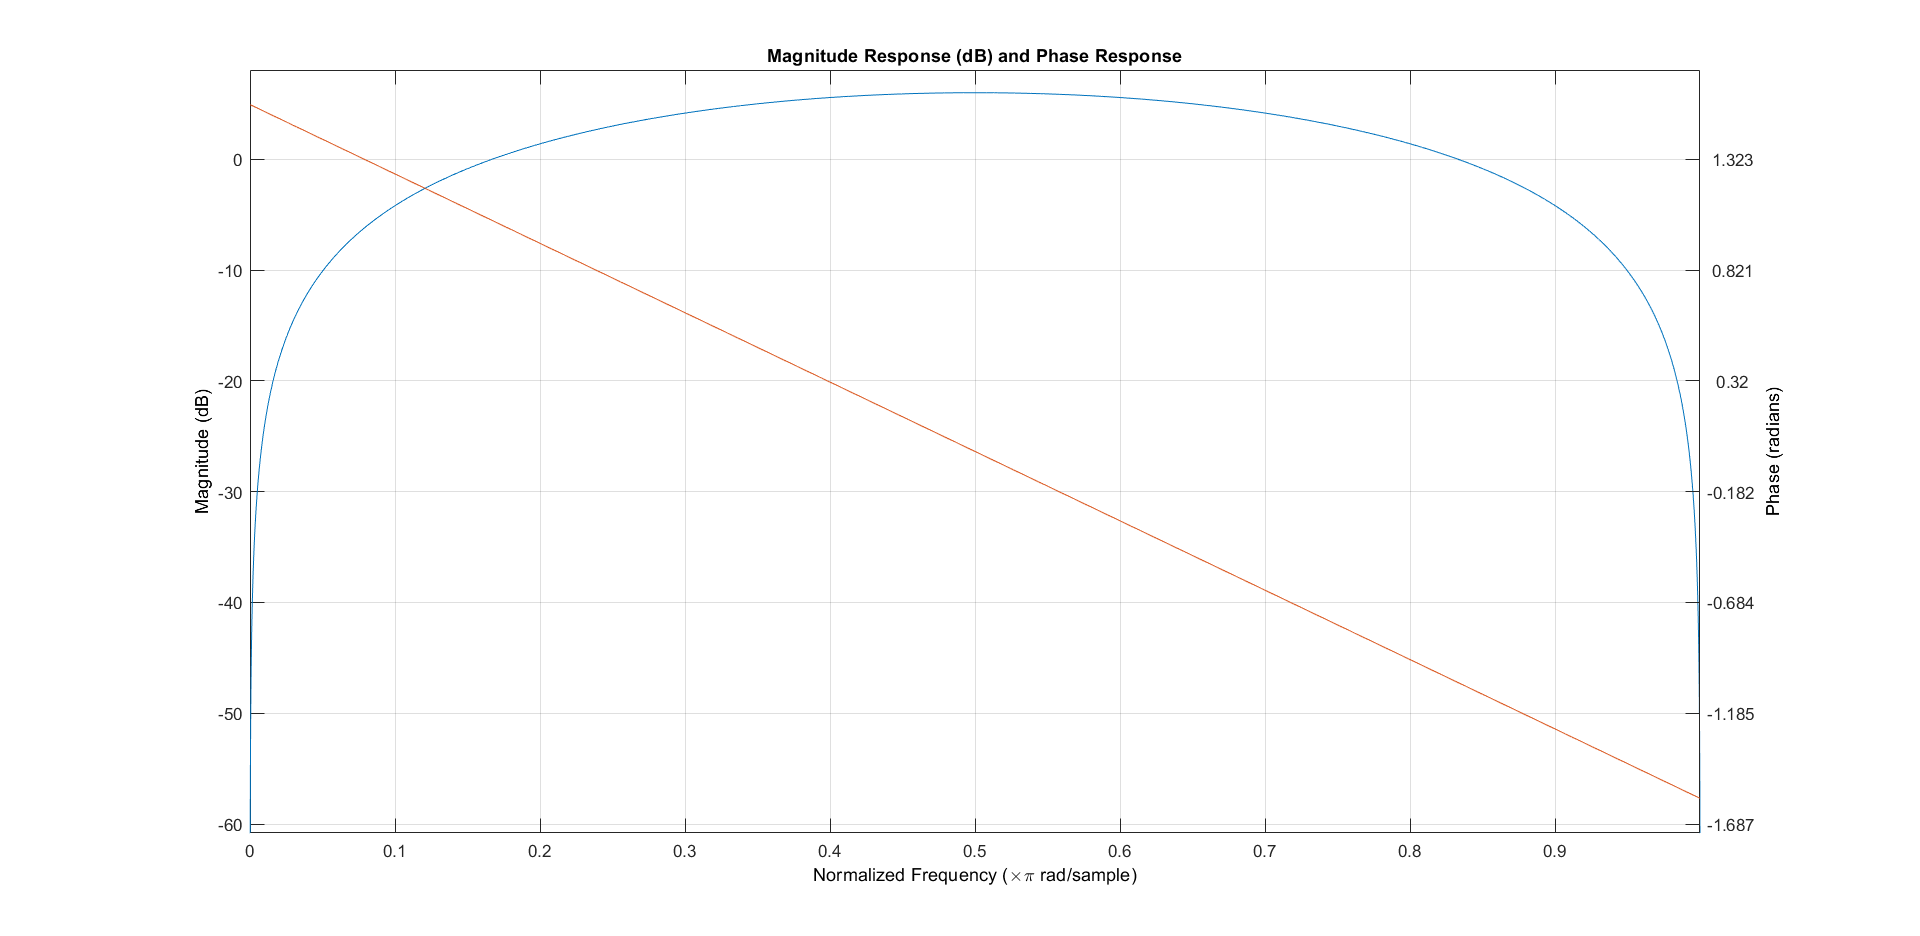
\includegraphics[width=1.0\linewidth]{res/4_1_ach.png}
		\caption{Частотные характеристики фильтра}
	\end{figure}
	
	Реализуем фильтр с $N = 5$.
	\begin{figure}[H]
		\centering
		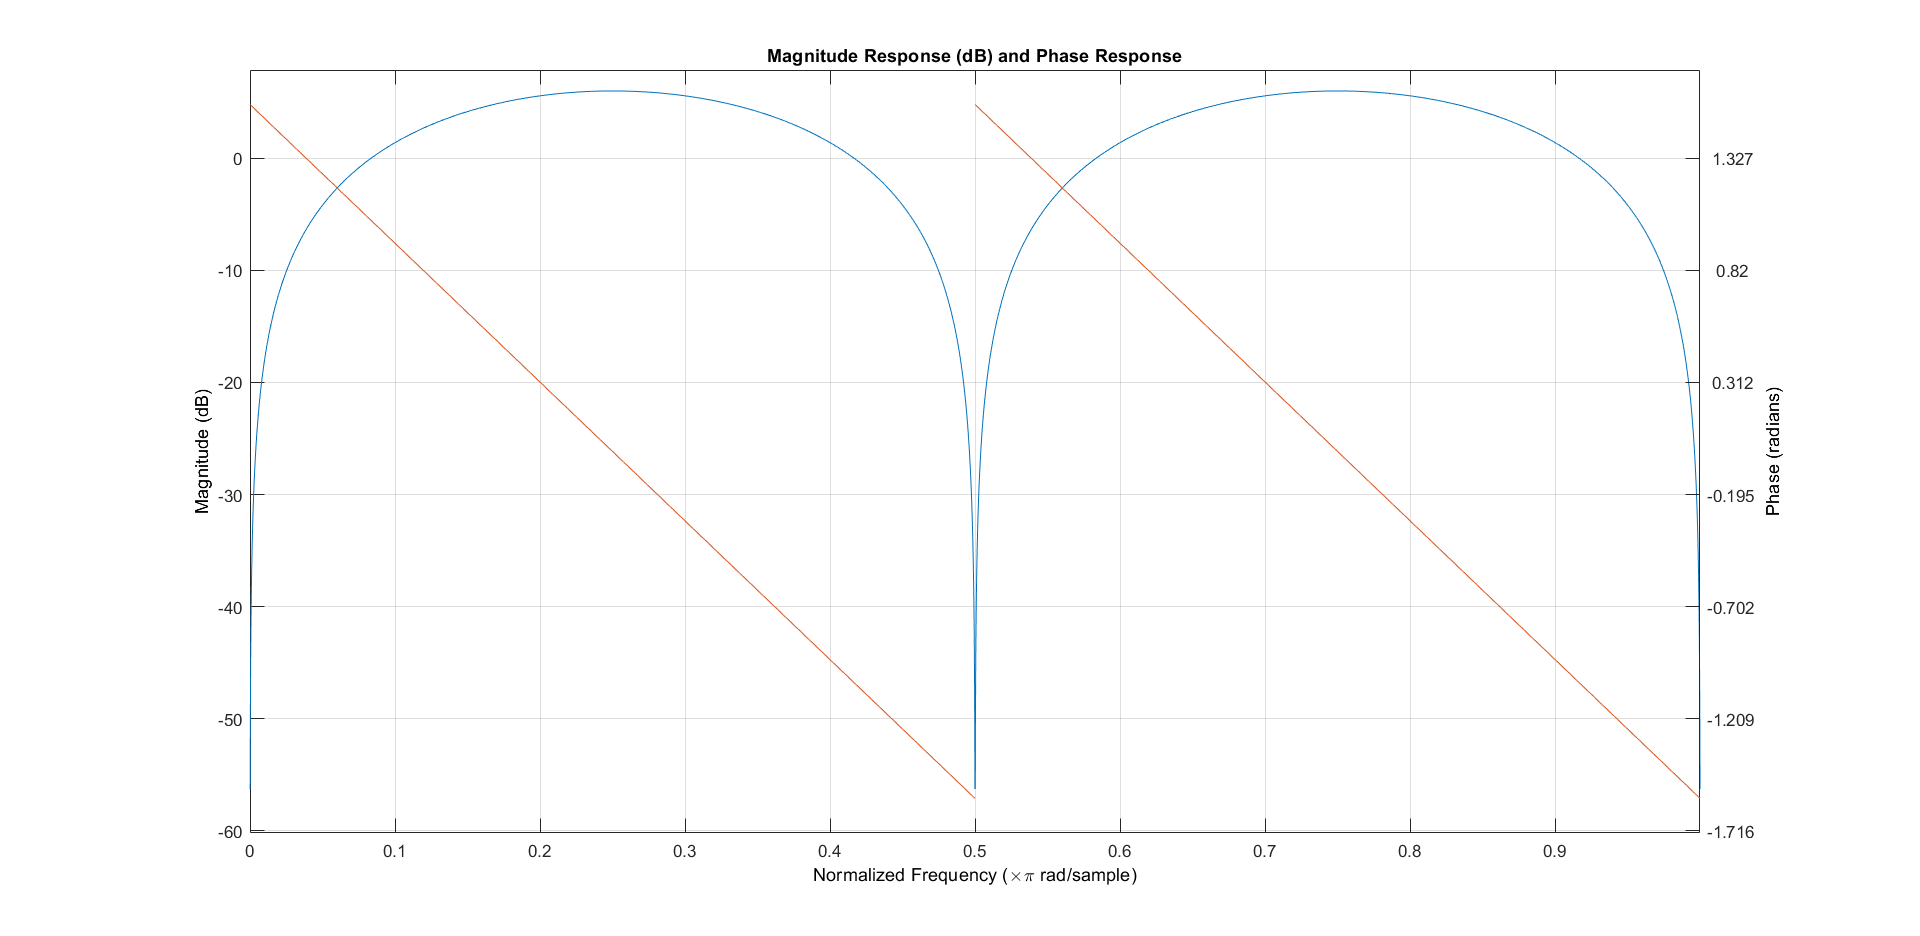
\includegraphics[width=1.0\linewidth]{res/4_1_N5.png}
		\caption{Частотные характеристики фильтра}
	\end{figure}
	
	Реализуем фильтр порядка $N = 7$ с прямоугольной импульсной реакцией.
	$$ h = [1, 1, 1, 1, 1, 1, 1], \; g = [1]$$
	\begin{figure}[H]
		\centering
		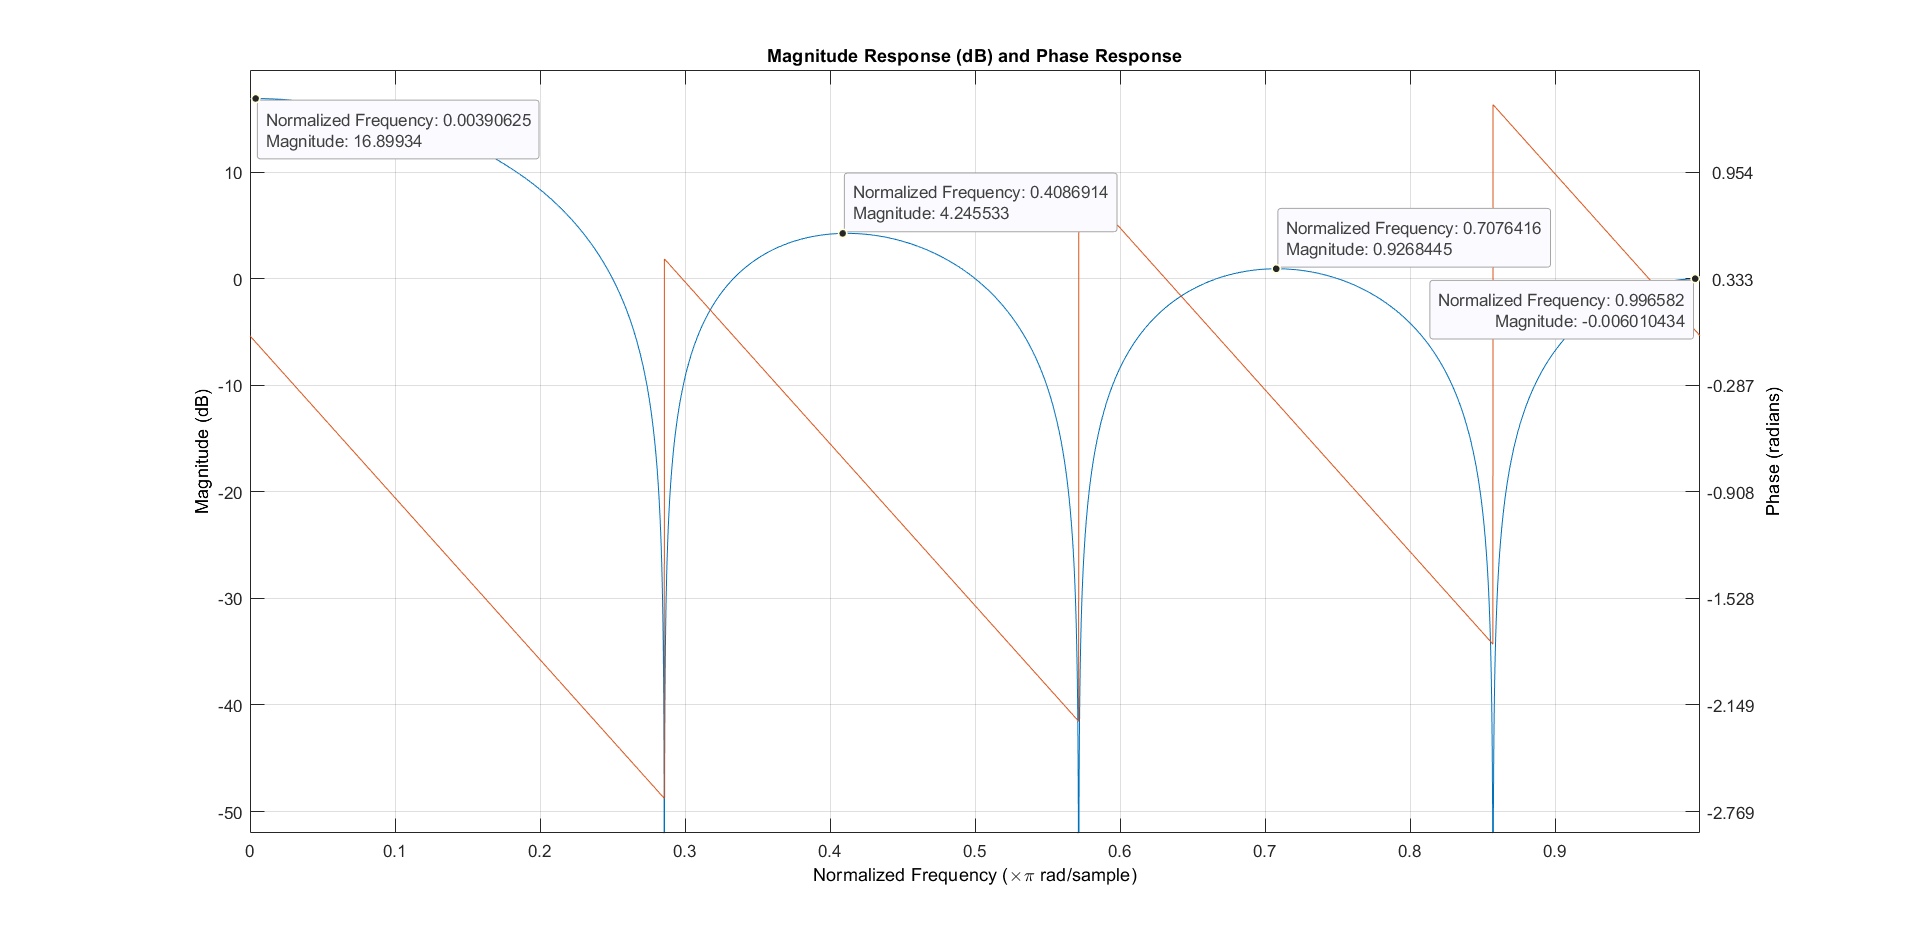
\includegraphics[width=1.0\linewidth]{res/4_2_N7.png}
		\caption{Частотные характеристики фильтра}
	\end{figure}
	Значения затухания в  пиках указаны на рисунке.
	
	Убедимся, что разницы в пиках почти не меняются, $N = 9$:
	\begin{figure}[H]
		\centering
		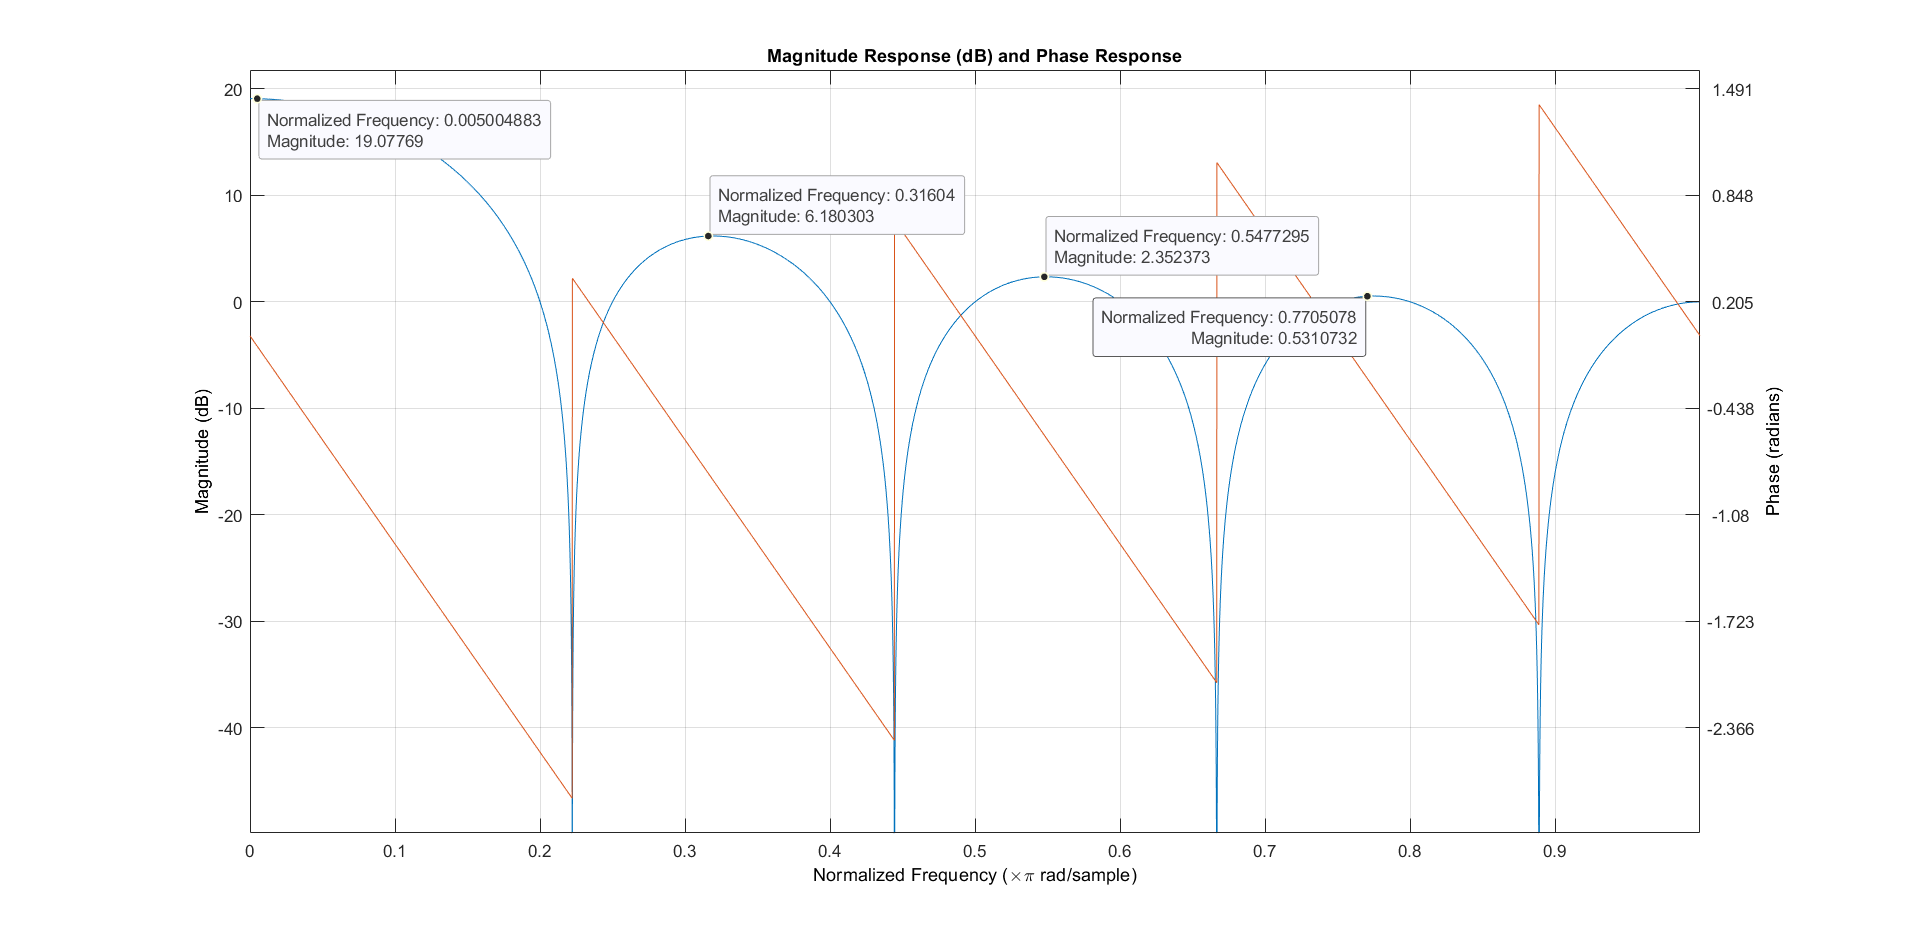
\includegraphics[width=1.0\linewidth]{res/4_2_N9.png}
		\caption{Частотные характеристики фильтра}
	\end{figure}
	
	Изменения в пределах $1 \; dB$.
	
	Такой же фильтр дает $h = [1, 0, 0, 0, 0, 0, 0, 0, -1], g = [1, -1]$.
	
	Рассмотрим временную характеристику:
	\begin{figure}[H]
		\centering
		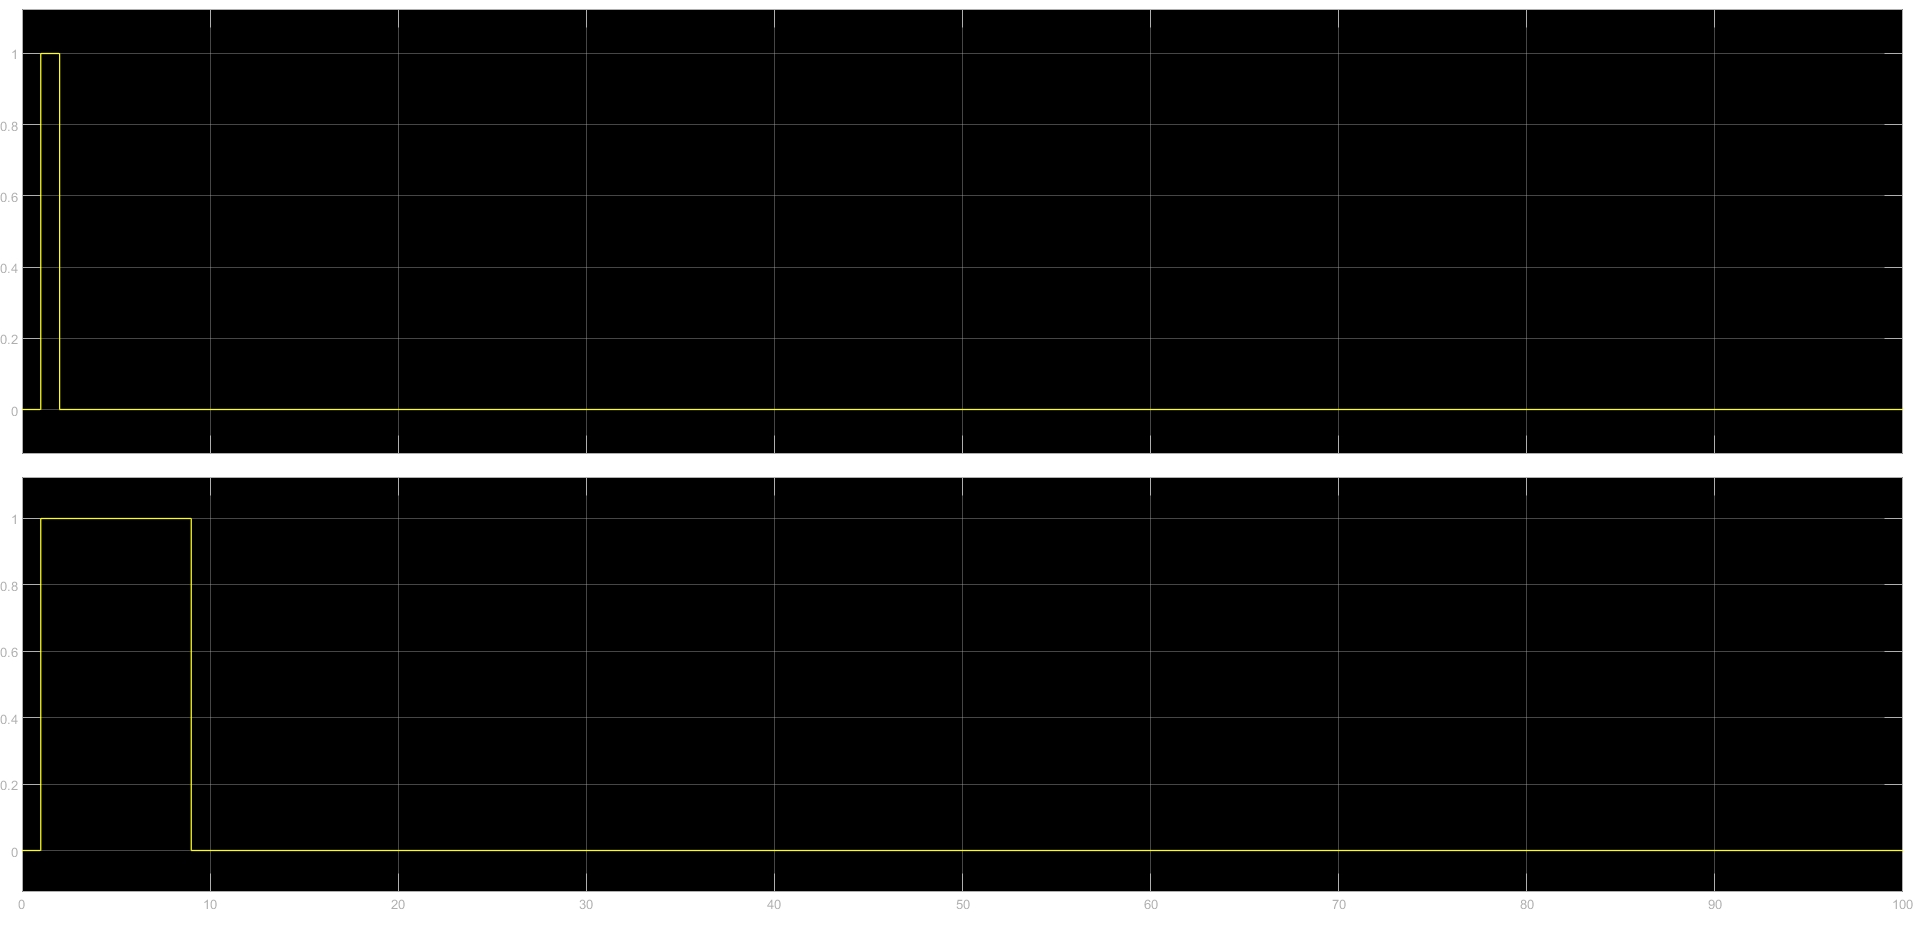
\includegraphics[width=1.0\linewidth]{res/4_2_impulse.png}
		\caption{Импульсная реакция фильтра}
	\end{figure}

	Подадим на фильтр $h = [1 1 1 1]$ шум и рассмотрим спектр после фильтра с децимацией $D = 4$ и без:
	\begin{figure}[H]
		\centering
		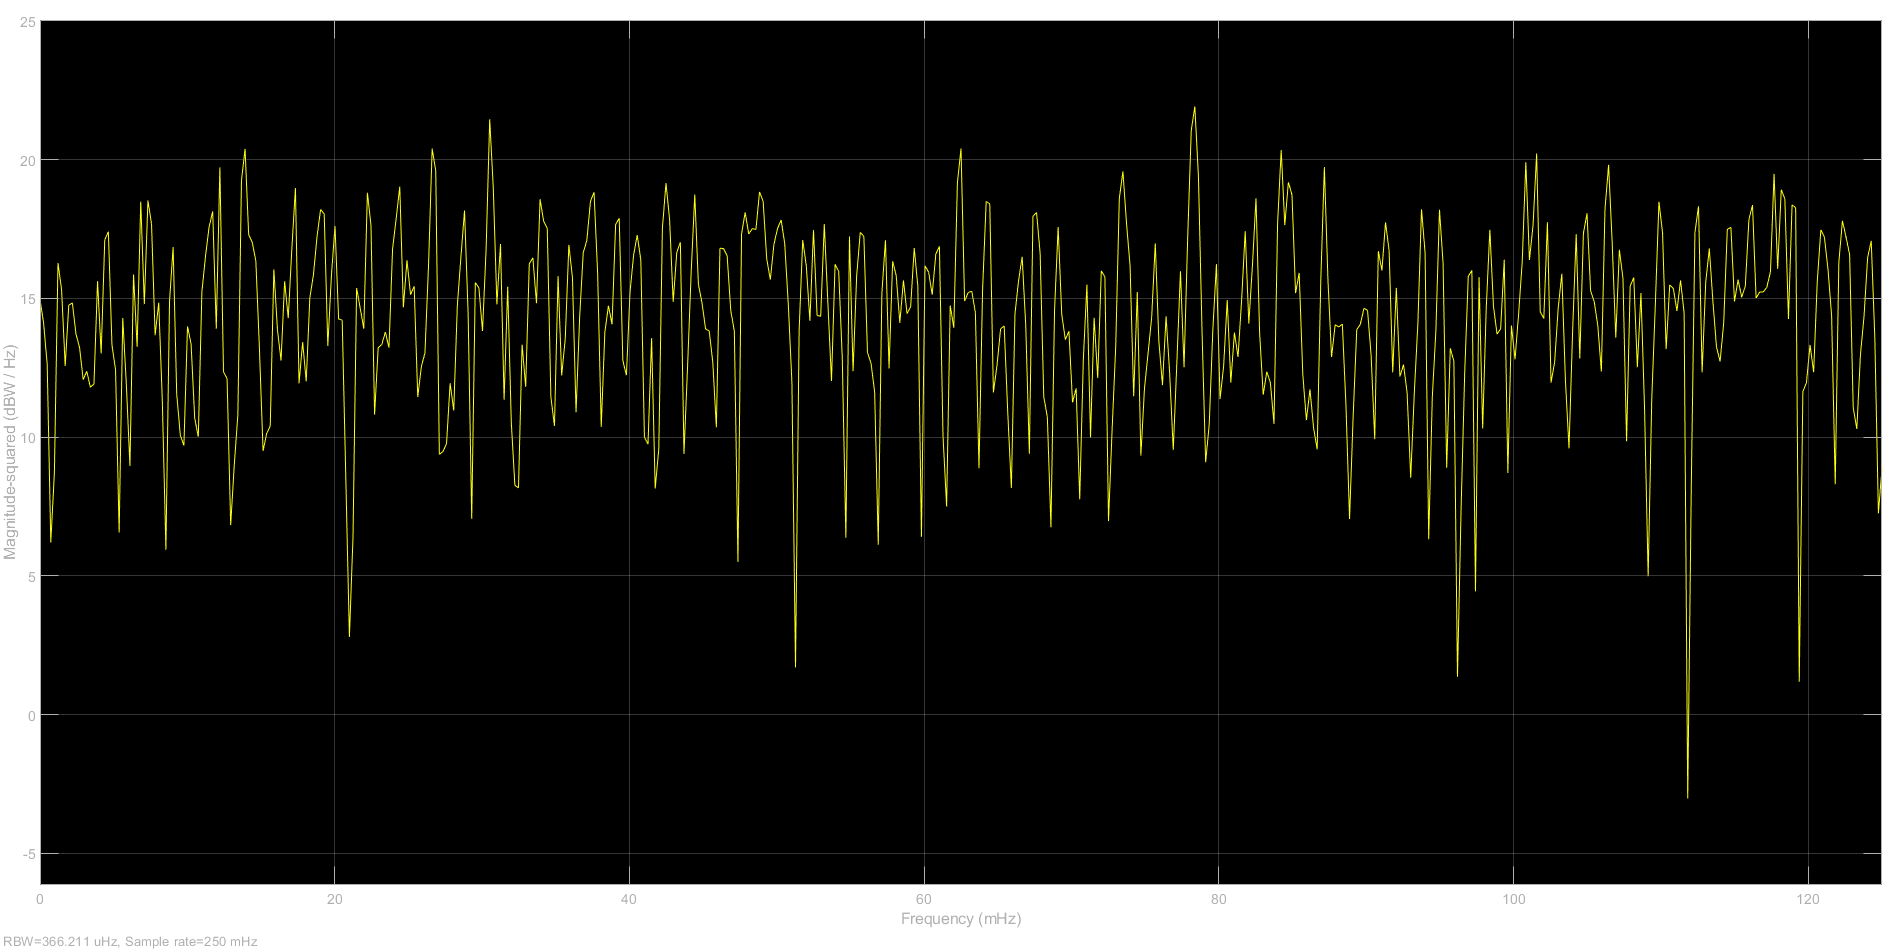
\includegraphics[width=1.0\linewidth]{res/4_3_N4_dec.png}
		\caption{Спектр фильтра с децимацией}
	\end{figure}
	\begin{figure}[H]
		\centering
		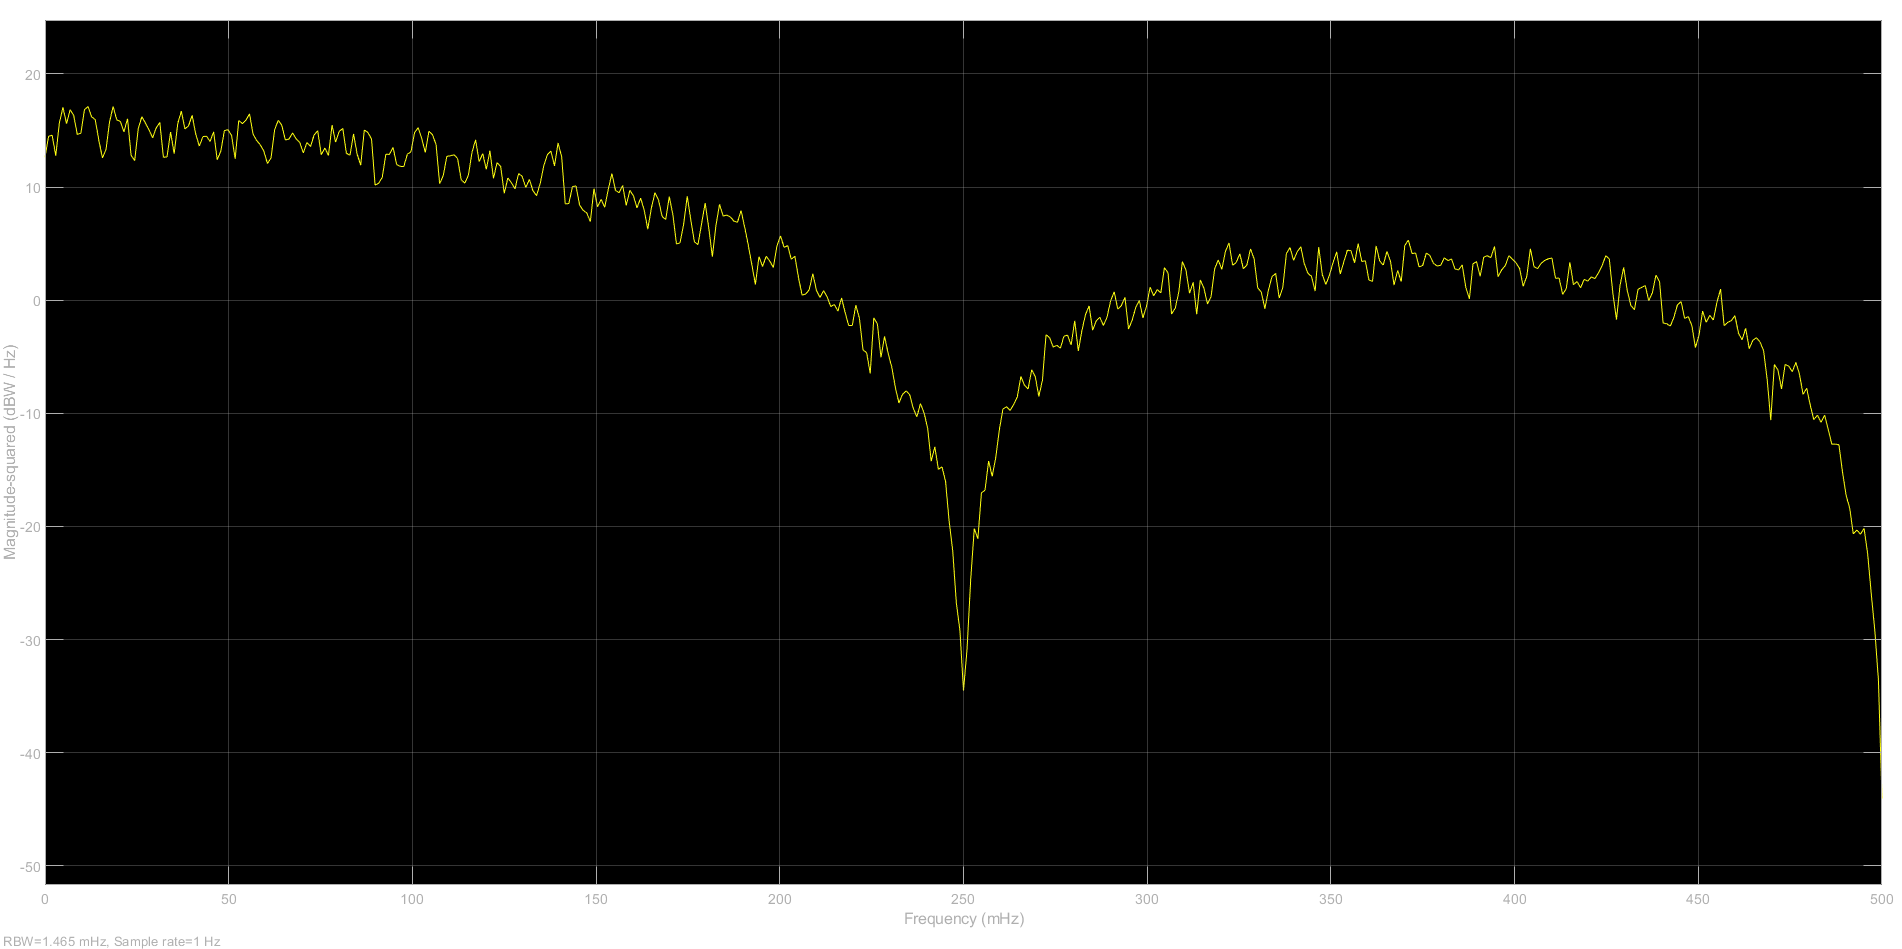
\includegraphics[width=1.0\linewidth]{res/4_3_N4.png}
		\caption{Спектр фильтра без децимации}
	\end{figure}
	Спектр равномерен, так как $0.5 / 4 \approx 0.125$ лежит в пределах плато первого пика фильтра и реплицируется в полосе Найквиста.
	
	Подадим на вход гармонический сигнал $f = 0.126/2$ ($\approx \pi/8$)
	\begin{figure}[H]
		\centering
		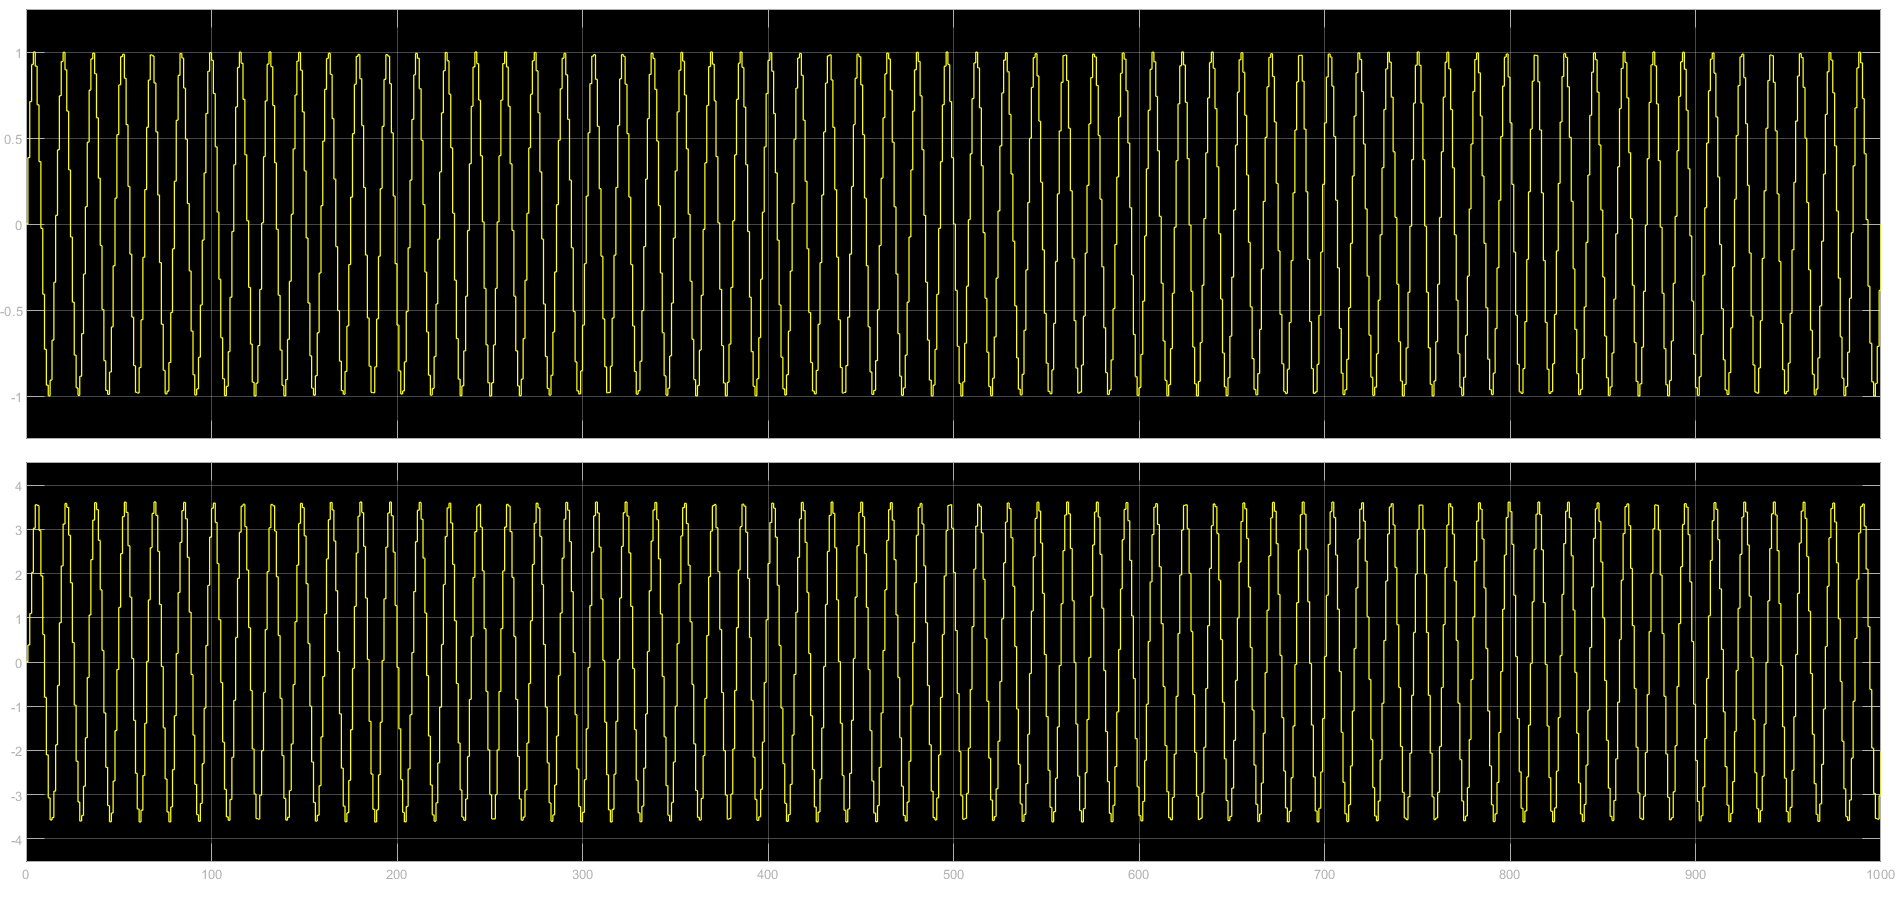
\includegraphics[width=1.0\linewidth]{res/4_4_inout_0126.png}
		\caption{Спектр фильтра без децимации}
	\end{figure}
	\begin{figure}[H]
		\centering
		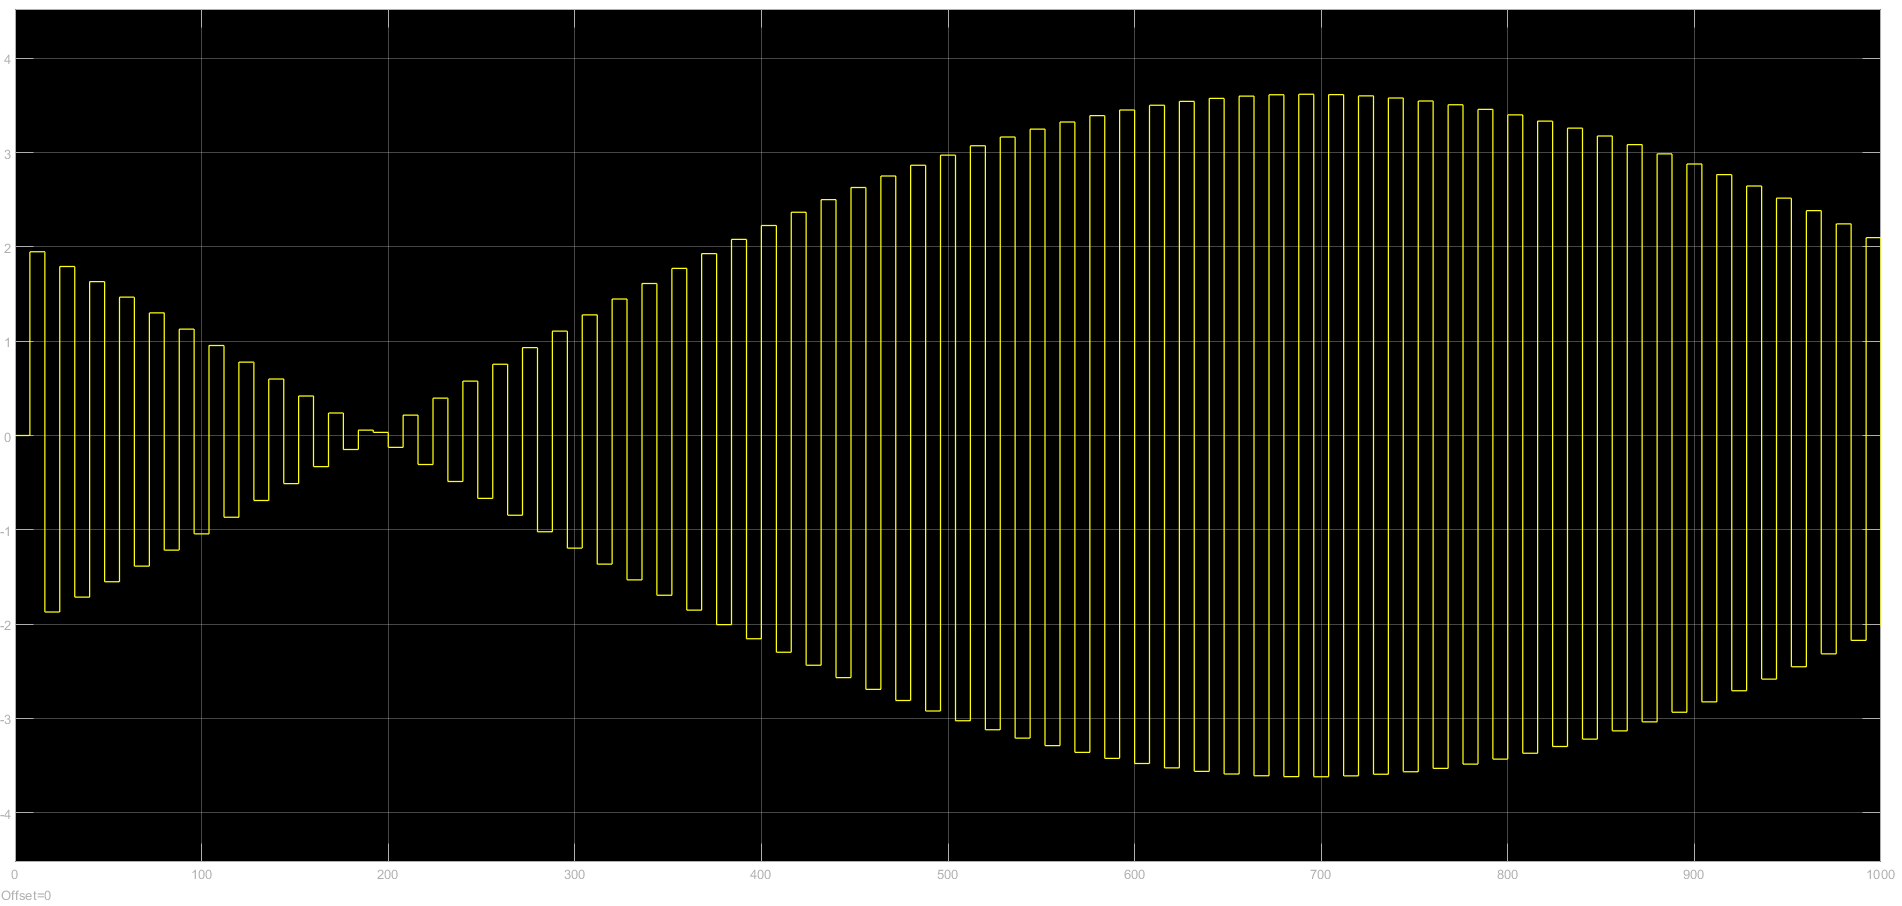
\includegraphics[width=1.0\linewidth]{res/4_4_dcm_0126.png}
		\caption{Спектр фильтра с децимацией}
	\end{figure}

	Подадим на вход гармонический сигнал $f = 1/2 + 0.126/2$ ($\approx \pi/2 + \pi/8$)
	\begin{figure}[H]
		\centering
		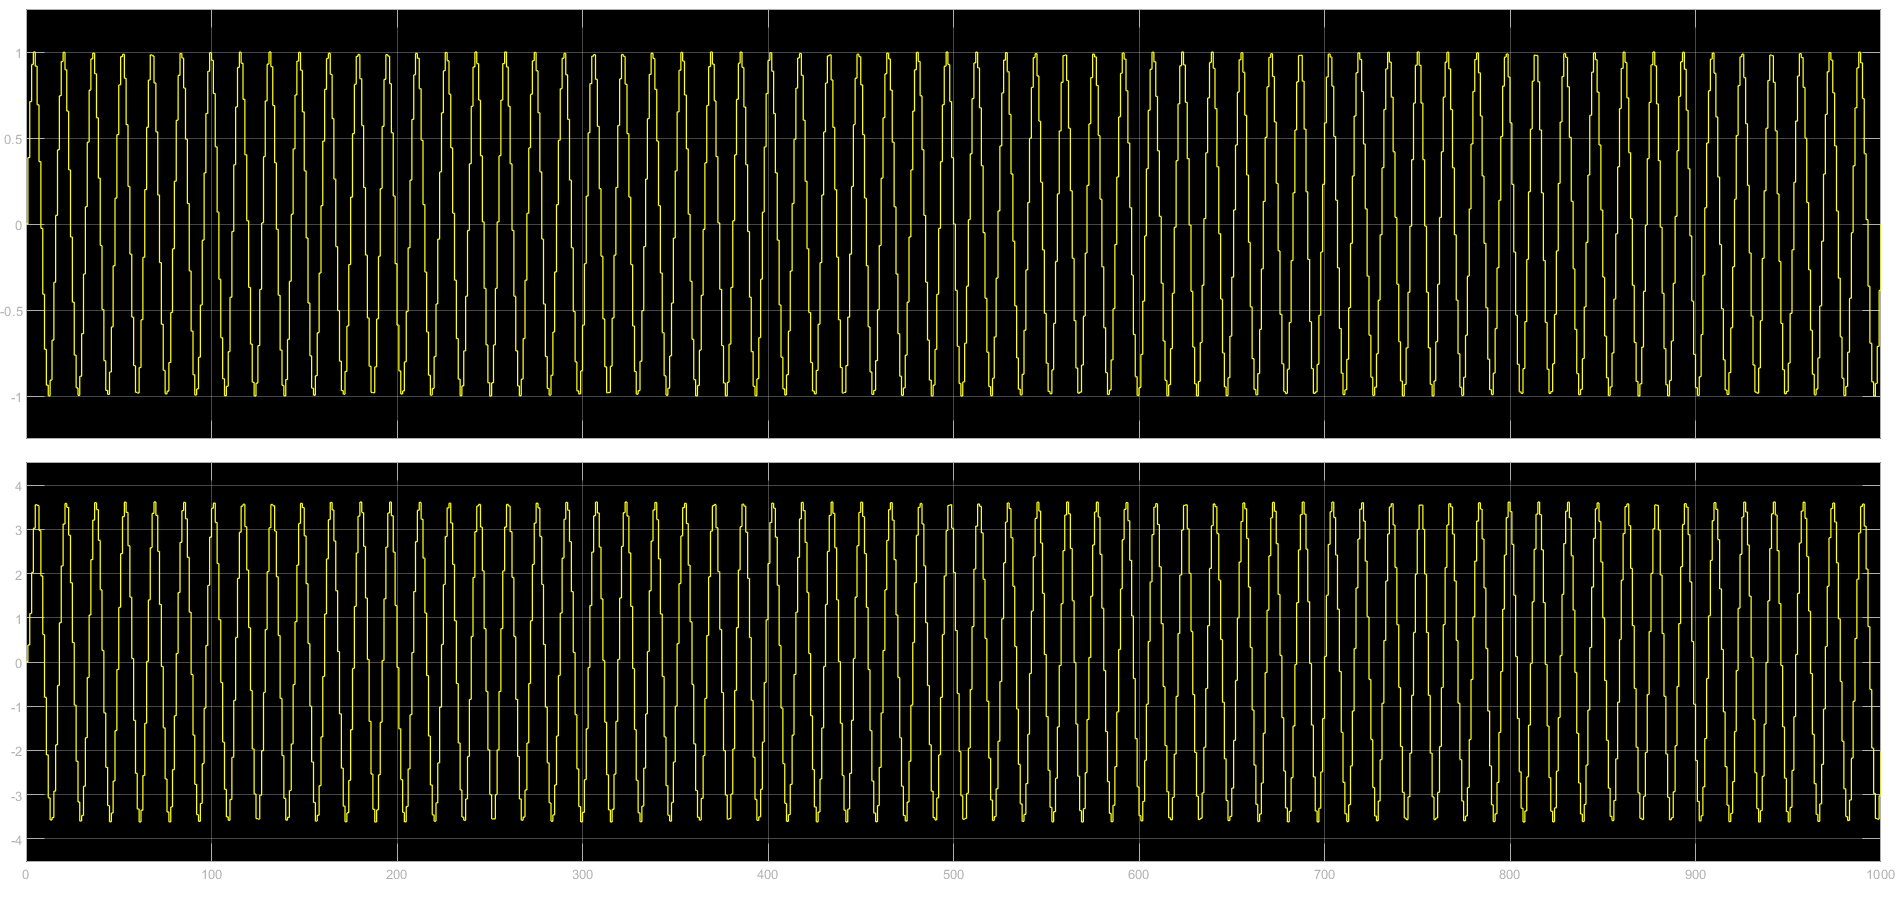
\includegraphics[width=1.0\linewidth]{res/4_4_inout_0126.png}
		\caption{Спектр фильтра без децимации}
	\end{figure}
	\begin{figure}[H]
		\centering
		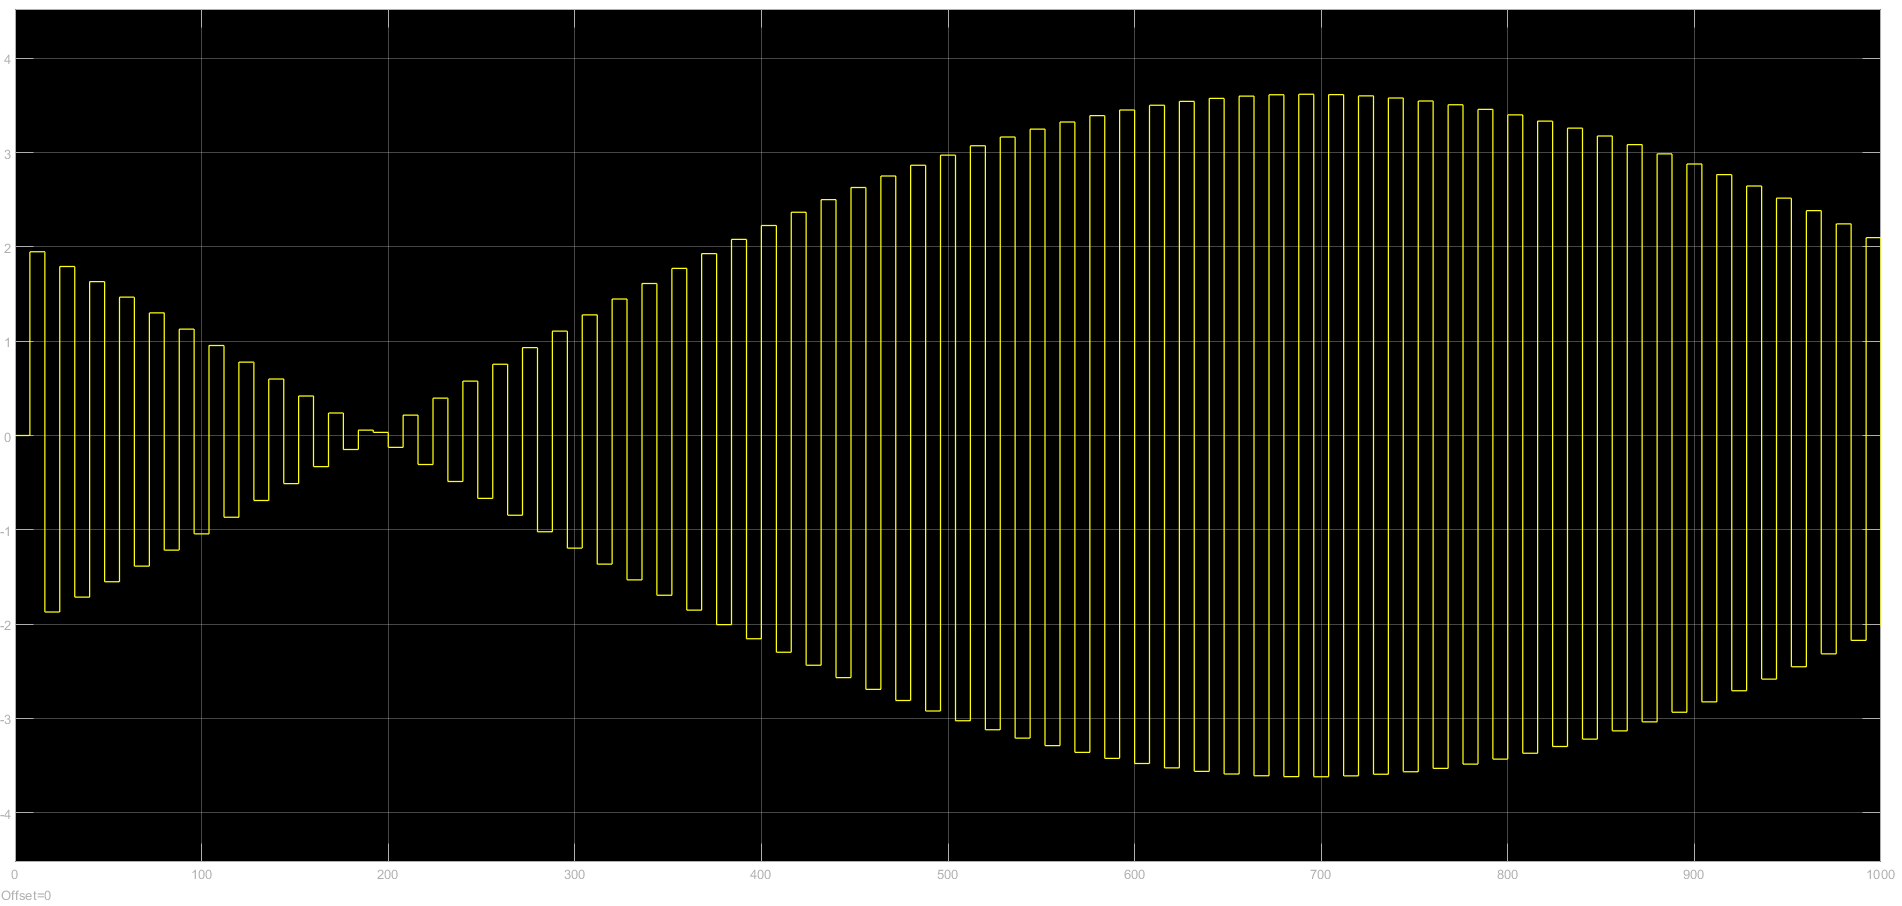
\includegraphics[width=1.0\linewidth]{res/4_4_dcm_0126.png}
		\caption{Спектр фильтра с децимацией}
	\end{figure}

	Подадим на вход гармонический сигнал $f = 1 + 0.126/2$ ($\approx \pi + \pi/8$)
	\begin{figure}[H]
		\centering
		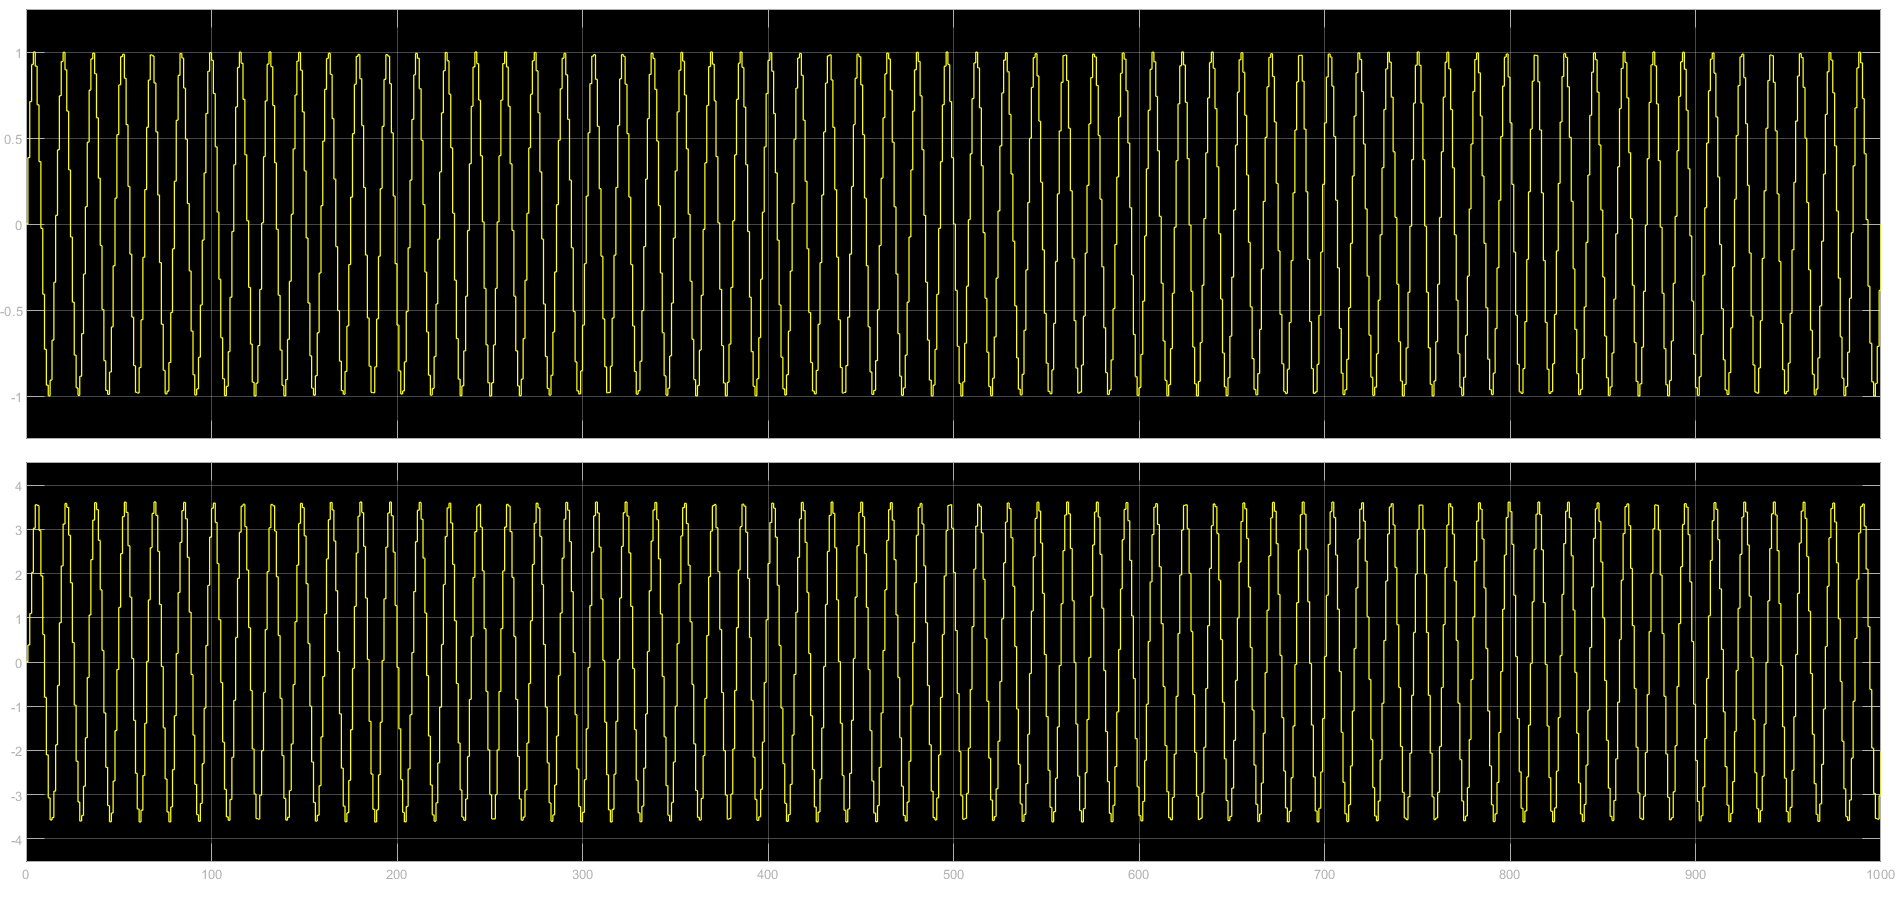
\includegraphics[width=1.0\linewidth]{res/4_4_inout_0126.png}
		\caption{Спектр фильтра без децимации}
	\end{figure}
	\begin{figure}[H]
		\centering
		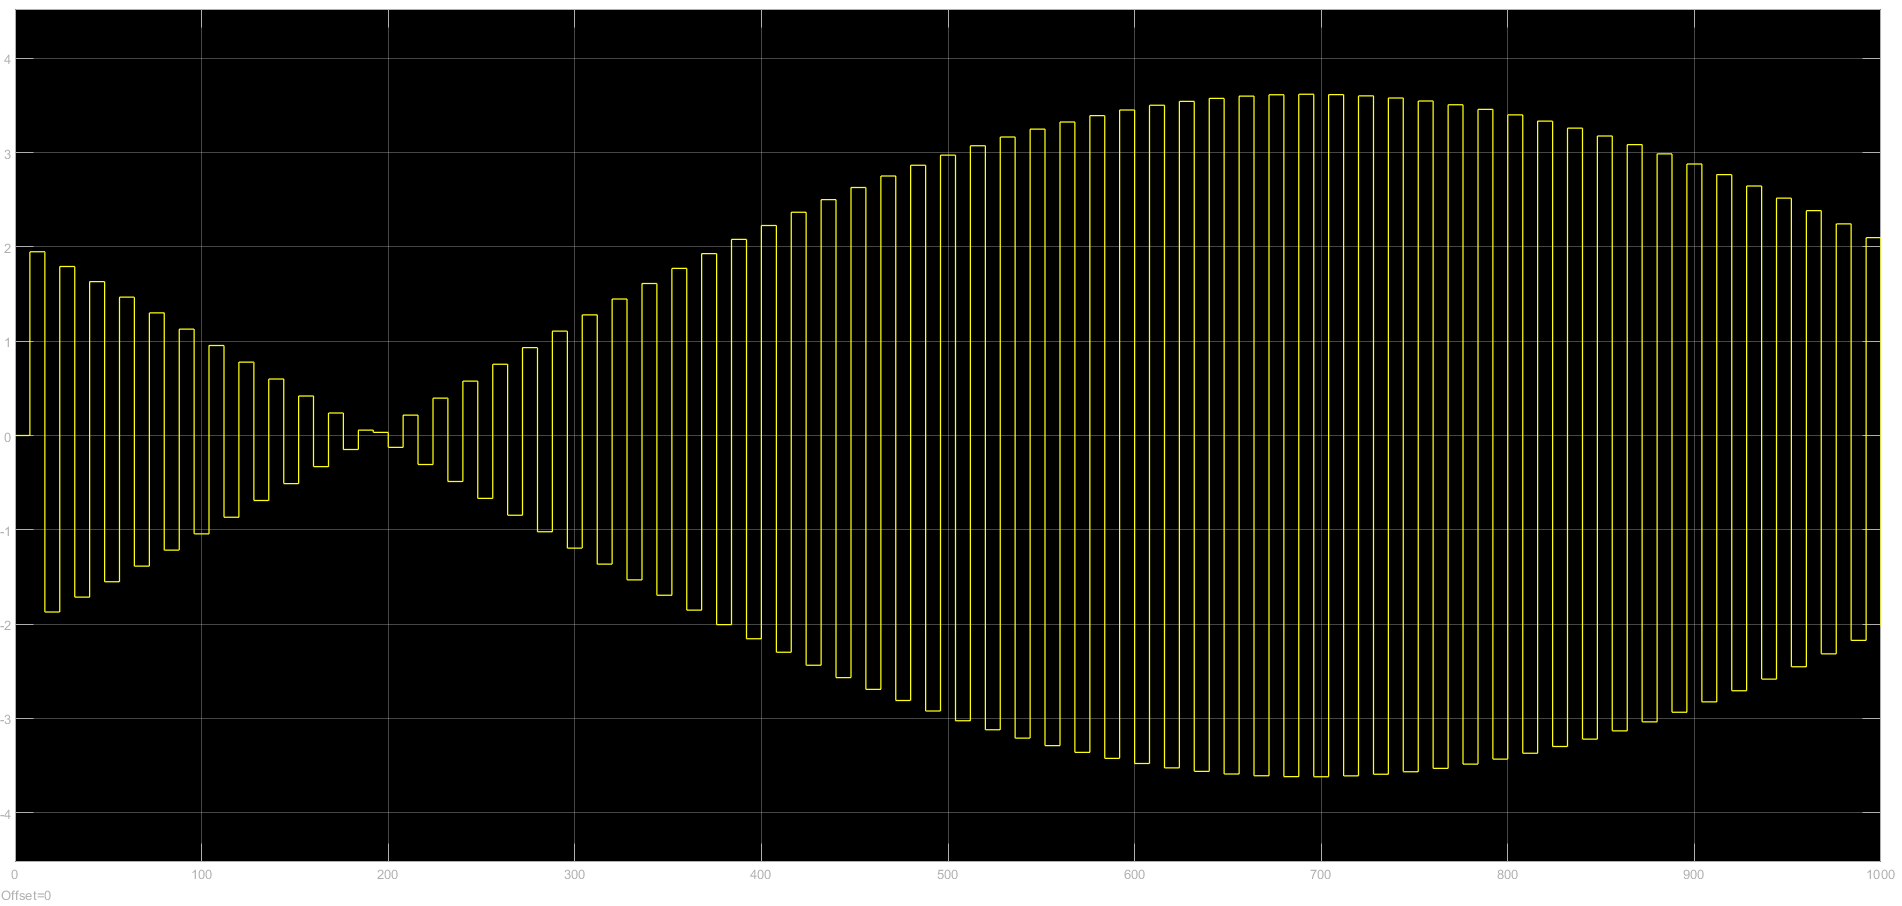
\includegraphics[width=1.0\linewidth]{res/4_4_dcm_0126.png}
		\caption{Спектр фильтра с децимацией}
	\end{figure}

	Рассмотрим FIR фильтры с временными окнами.

	\begin{figure}[H]
		\centering
		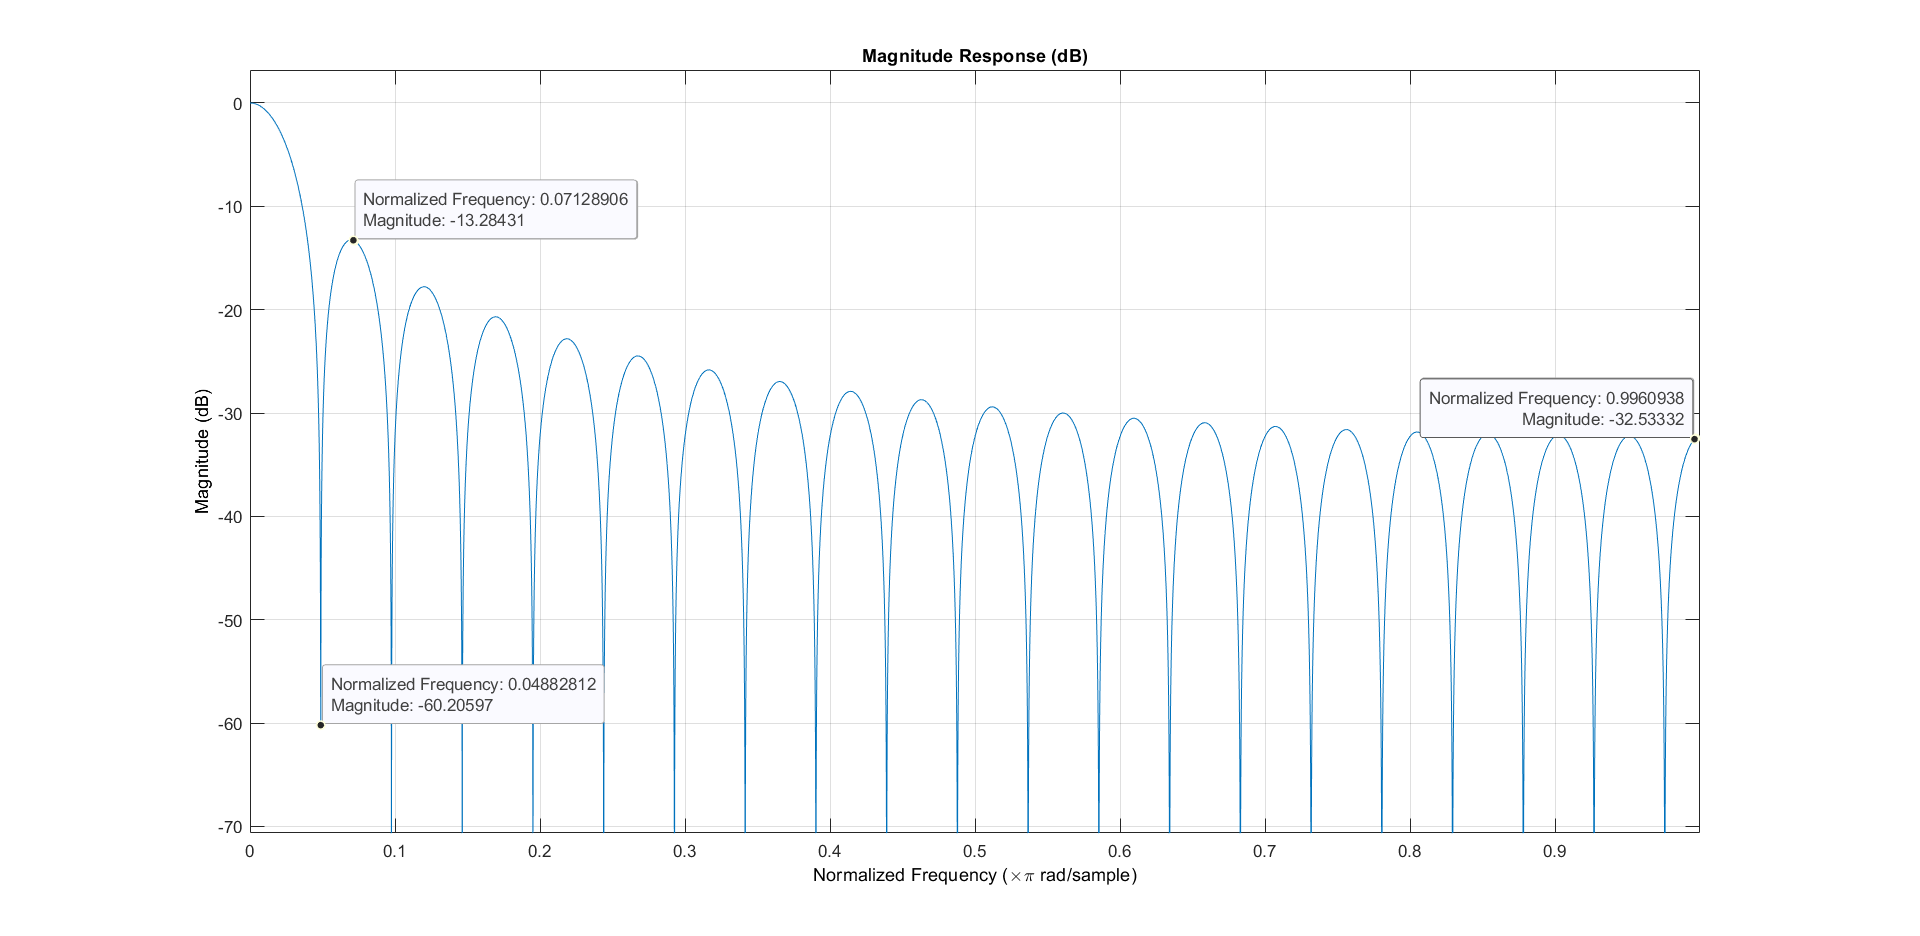
\includegraphics[width=1.0\linewidth]{res/4_5_N20_r.png}
		\caption{Спектр FIR фильтра, прямоугольное окно}
	\end{figure}
	
	\begin{figure}[H]
		\centering
		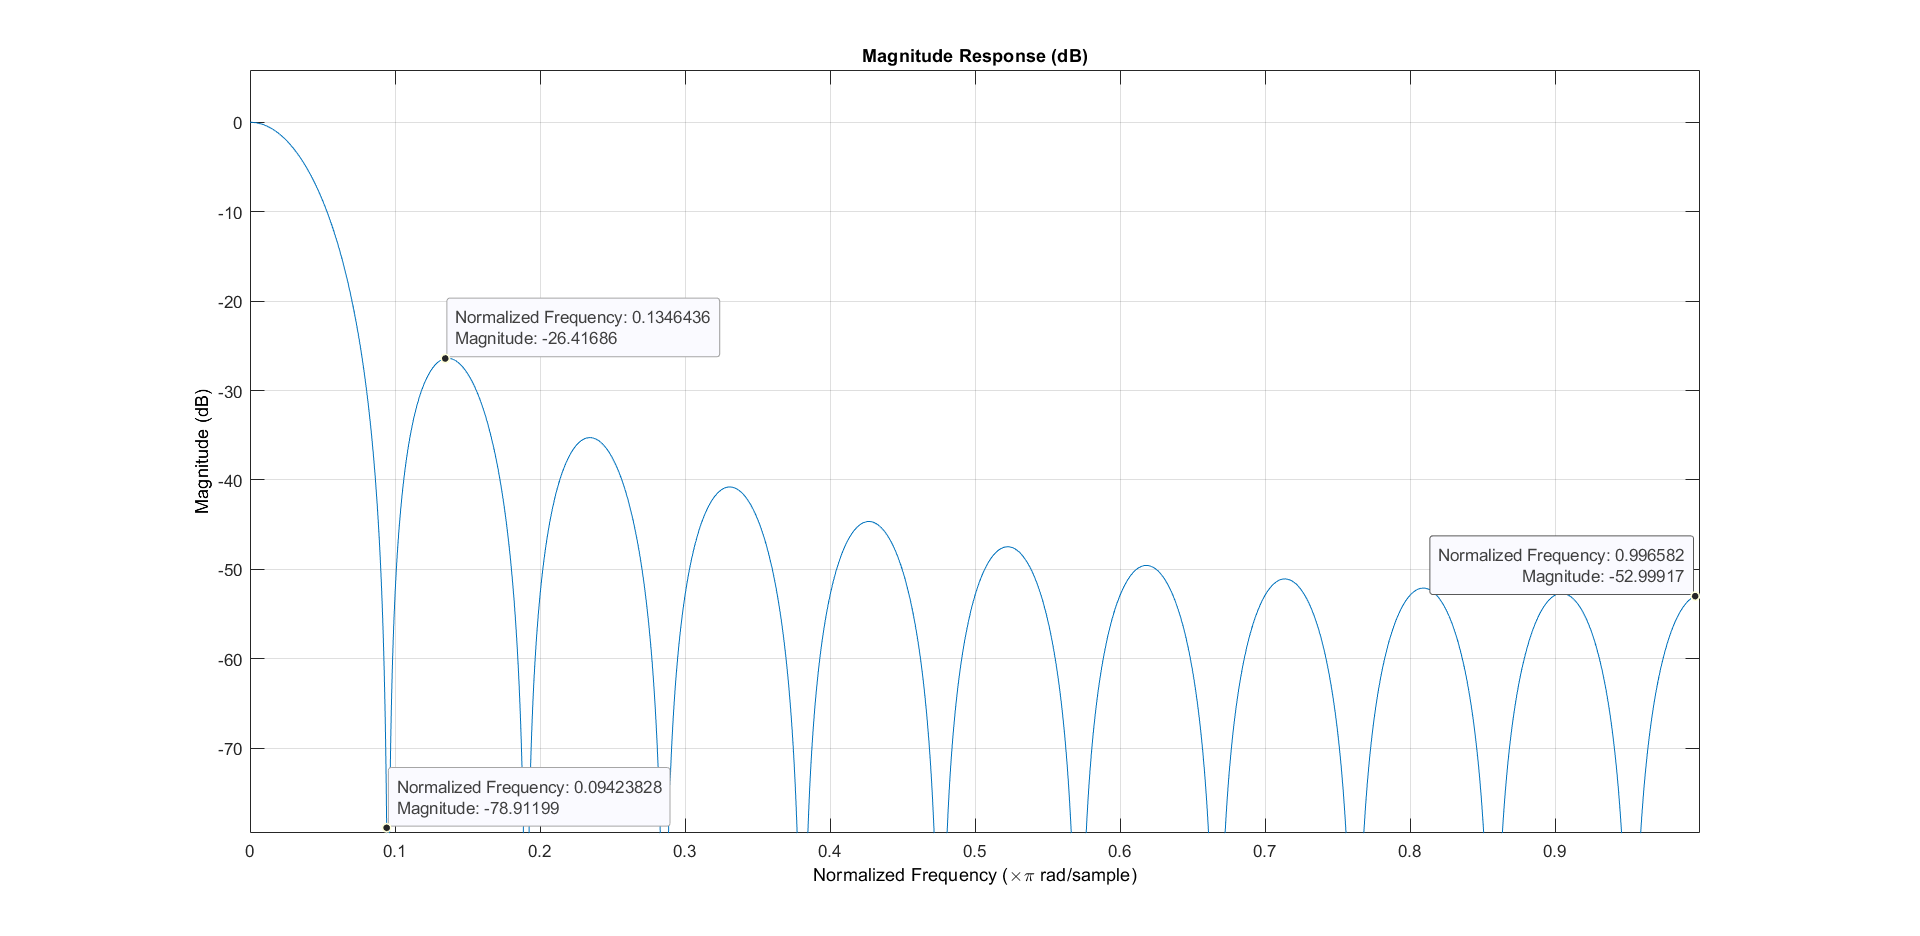
\includegraphics[width=1.0\linewidth]{res/4_5_N20_t.png}
		\caption{Спектр FIR фильтра, треугольное окно}
	\end{figure}
	
	\begin{figure}[H]
		\centering
		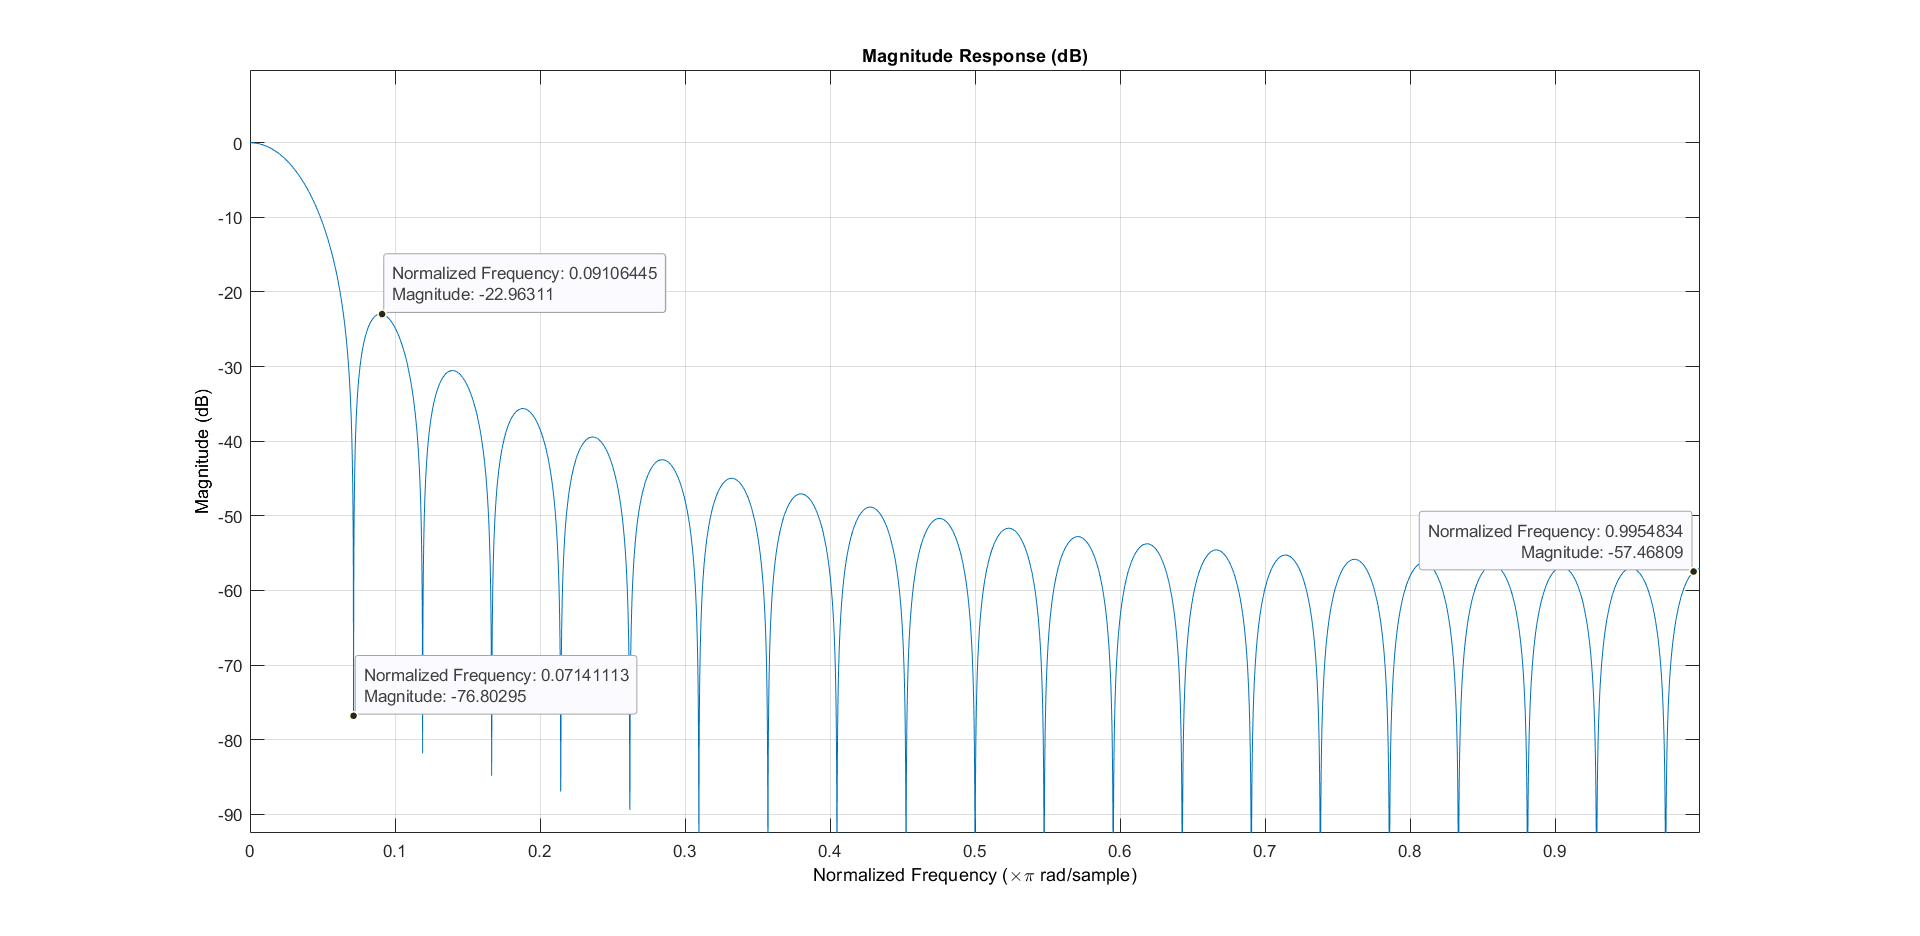
\includegraphics[width=1.0\linewidth]{res/4_5_N20_s.png}
		\caption{Спектр FIR фильтра, гармоническая полуволна}
	\end{figure}
	
	\begin{figure}[H]
		\centering
		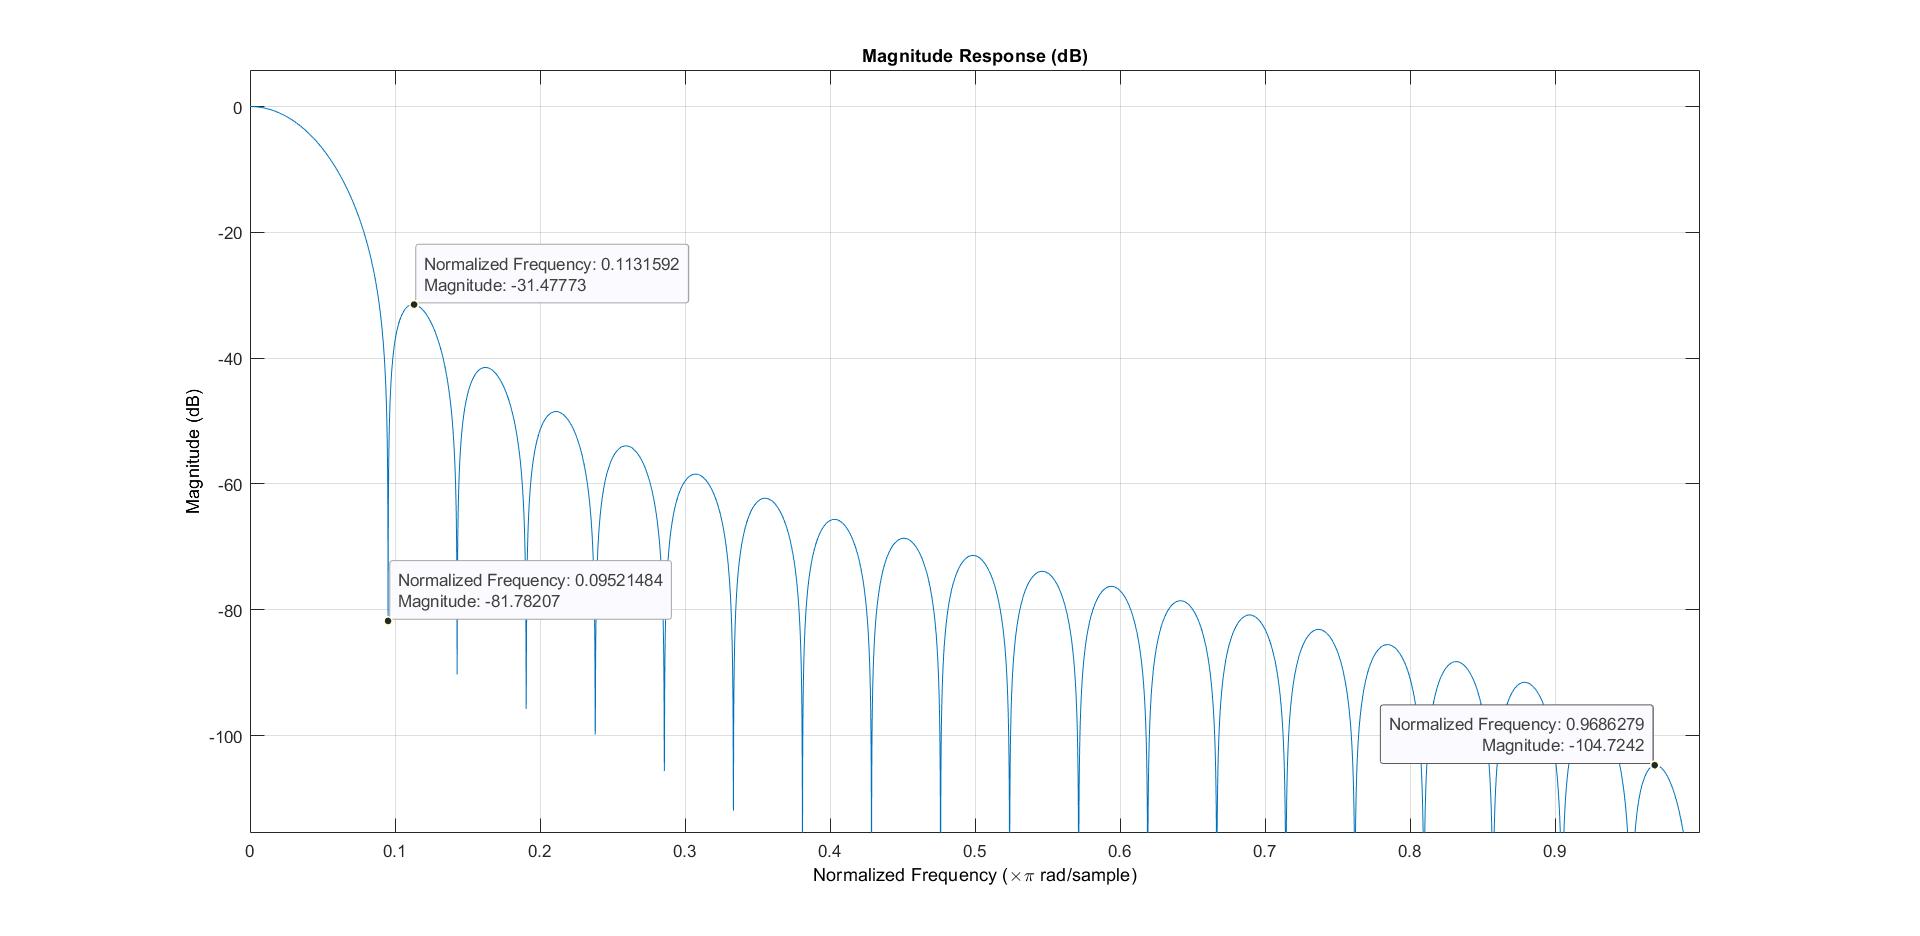
\includegraphics[width=1.0\linewidth]{res/4_5_N20_c.png}
		\caption{Спектр FIR фильтра, приподнятый косинус}
	\end{figure}
	
	\subsection*{5. FDATool Matlab}
	
	Синтезируем FIR-фильтр нижних частот с характеристиками:
	$$ wpass = 0.4 \qquad wstop = 0.5 \qquad Apass = 1 \qquad Astop = 60$$
	
	\begin{figure}[H]
		\centering
		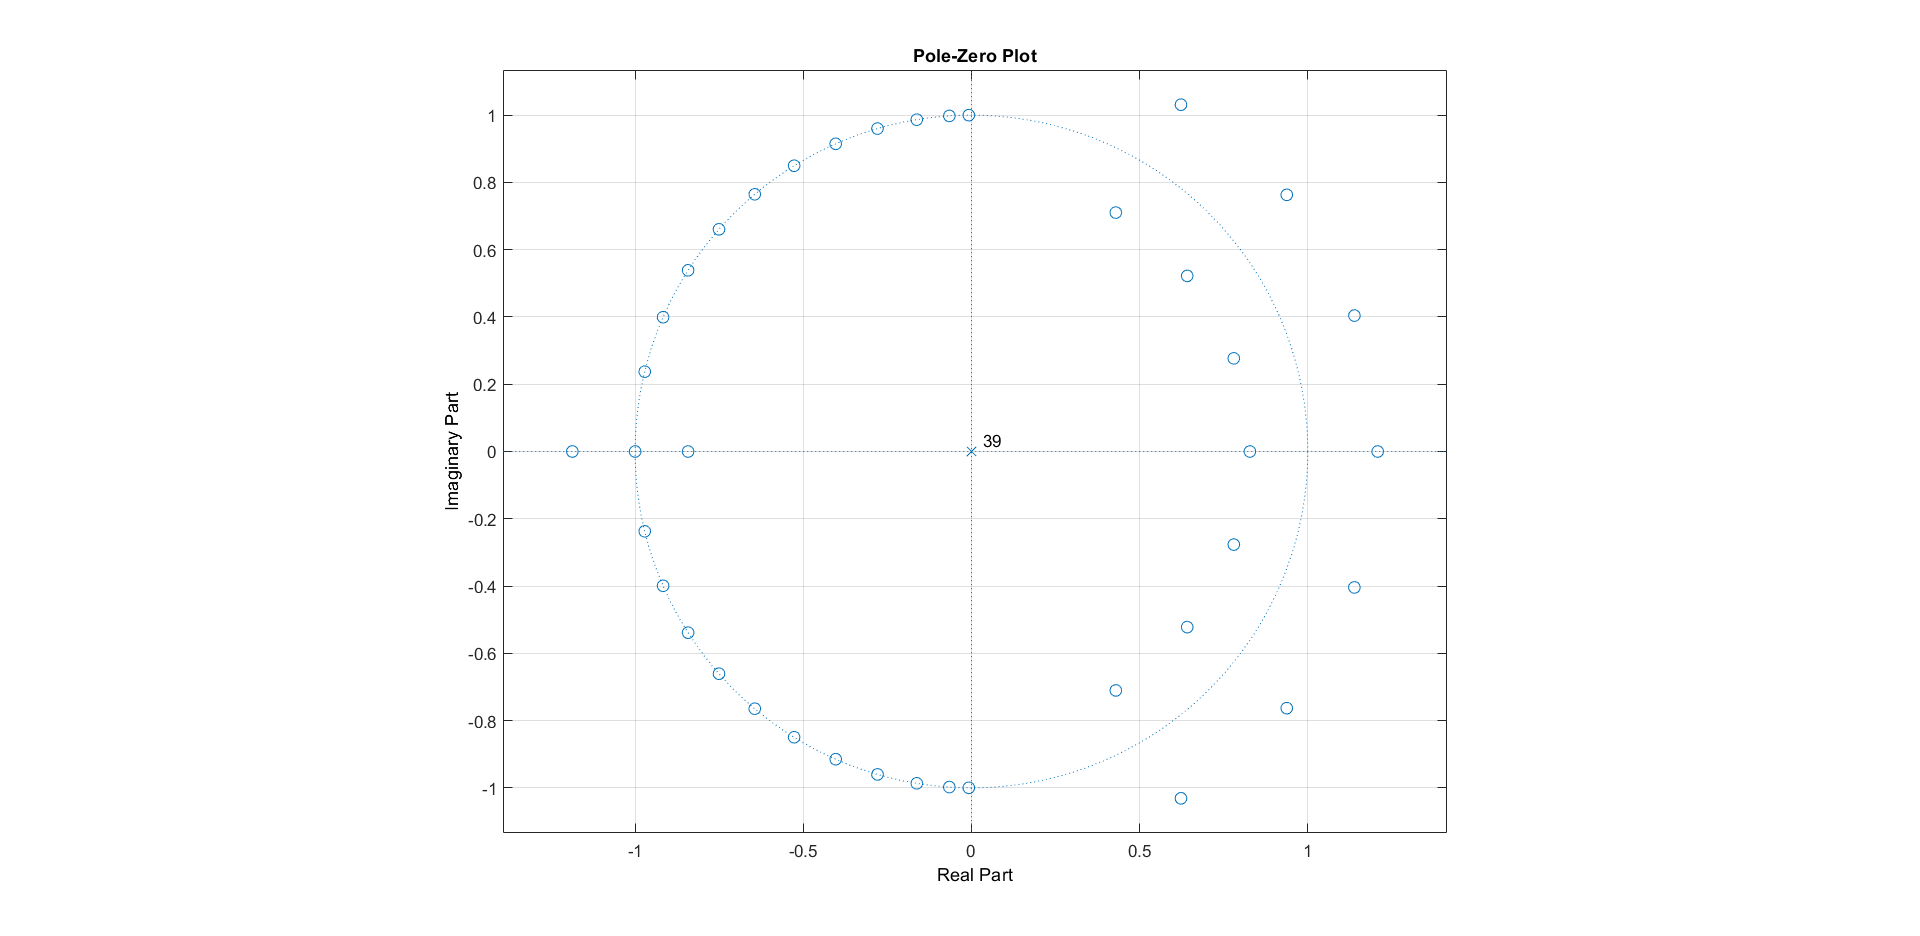
\includegraphics[width=1.0\linewidth]{res/5_fir_poles.png}
		\caption{Карта полюсов FIR фильтра}
	\end{figure}
	
	\begin{figure}[H]
		\centering
		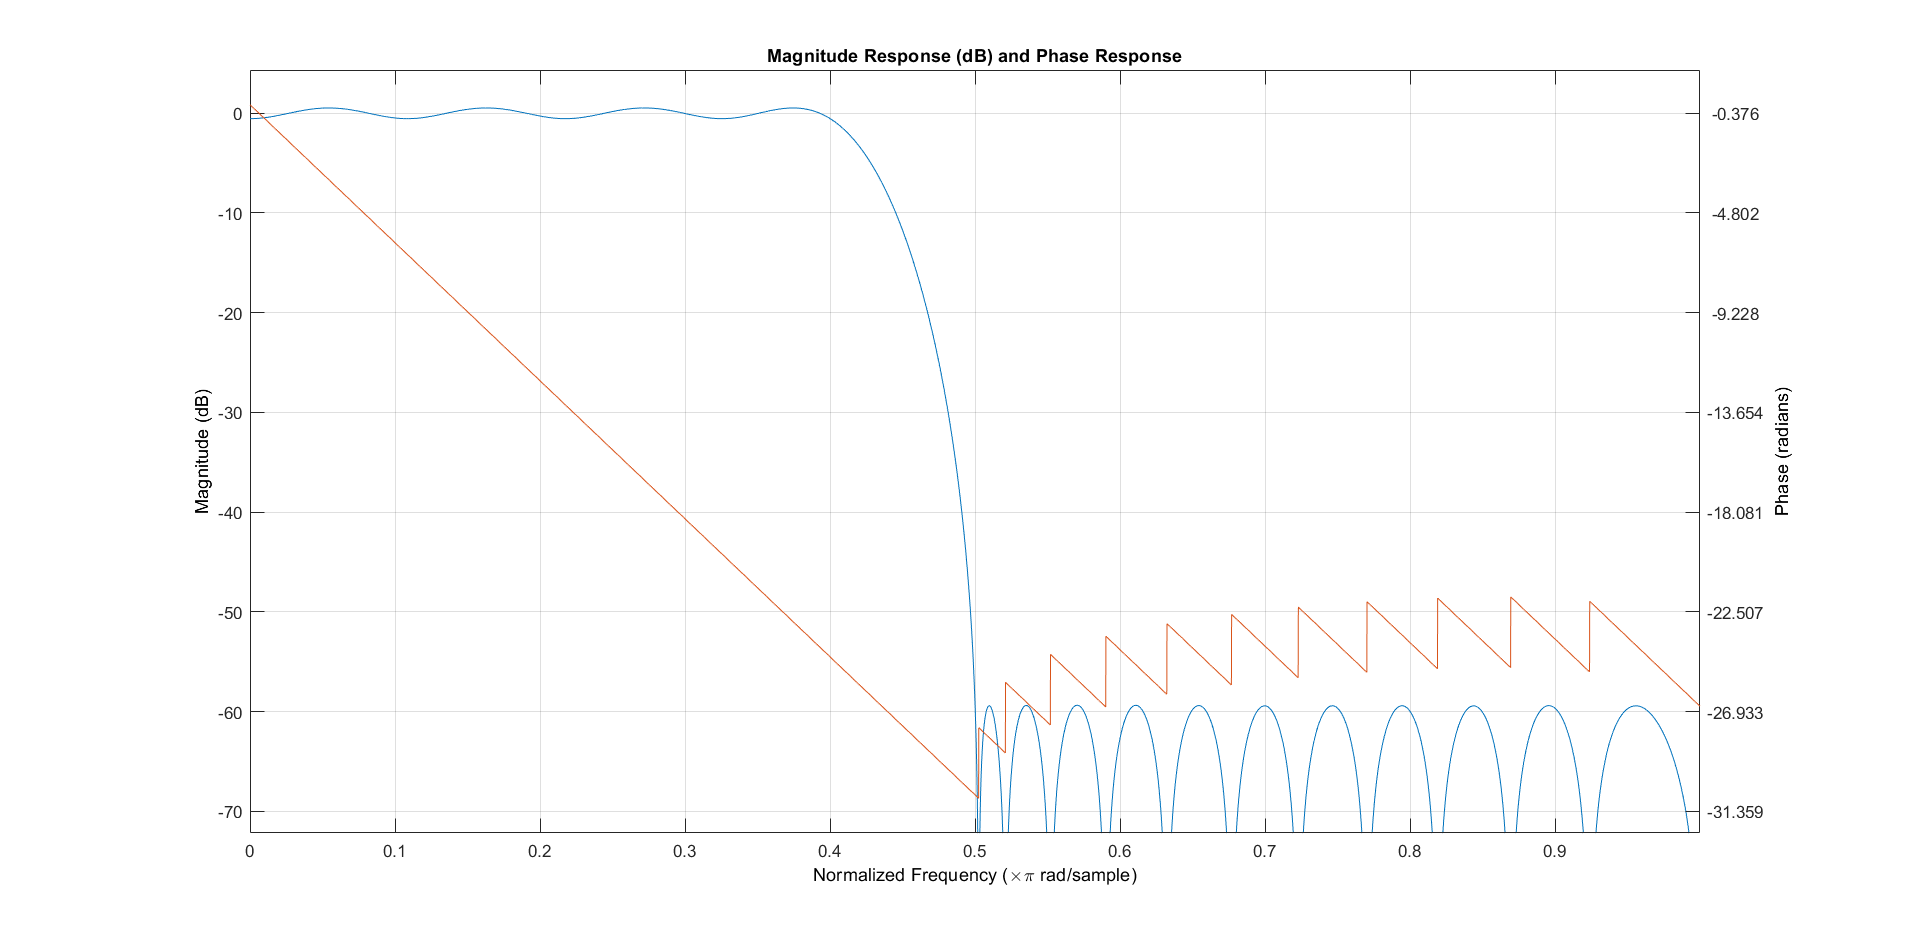
\includegraphics[width=1.0\linewidth]{res/5_fir_ach.png}
		\caption{Частотные характеристики FIR фильтра}
	\end{figure}
		
	\begin{figure}[H]
		\centering
		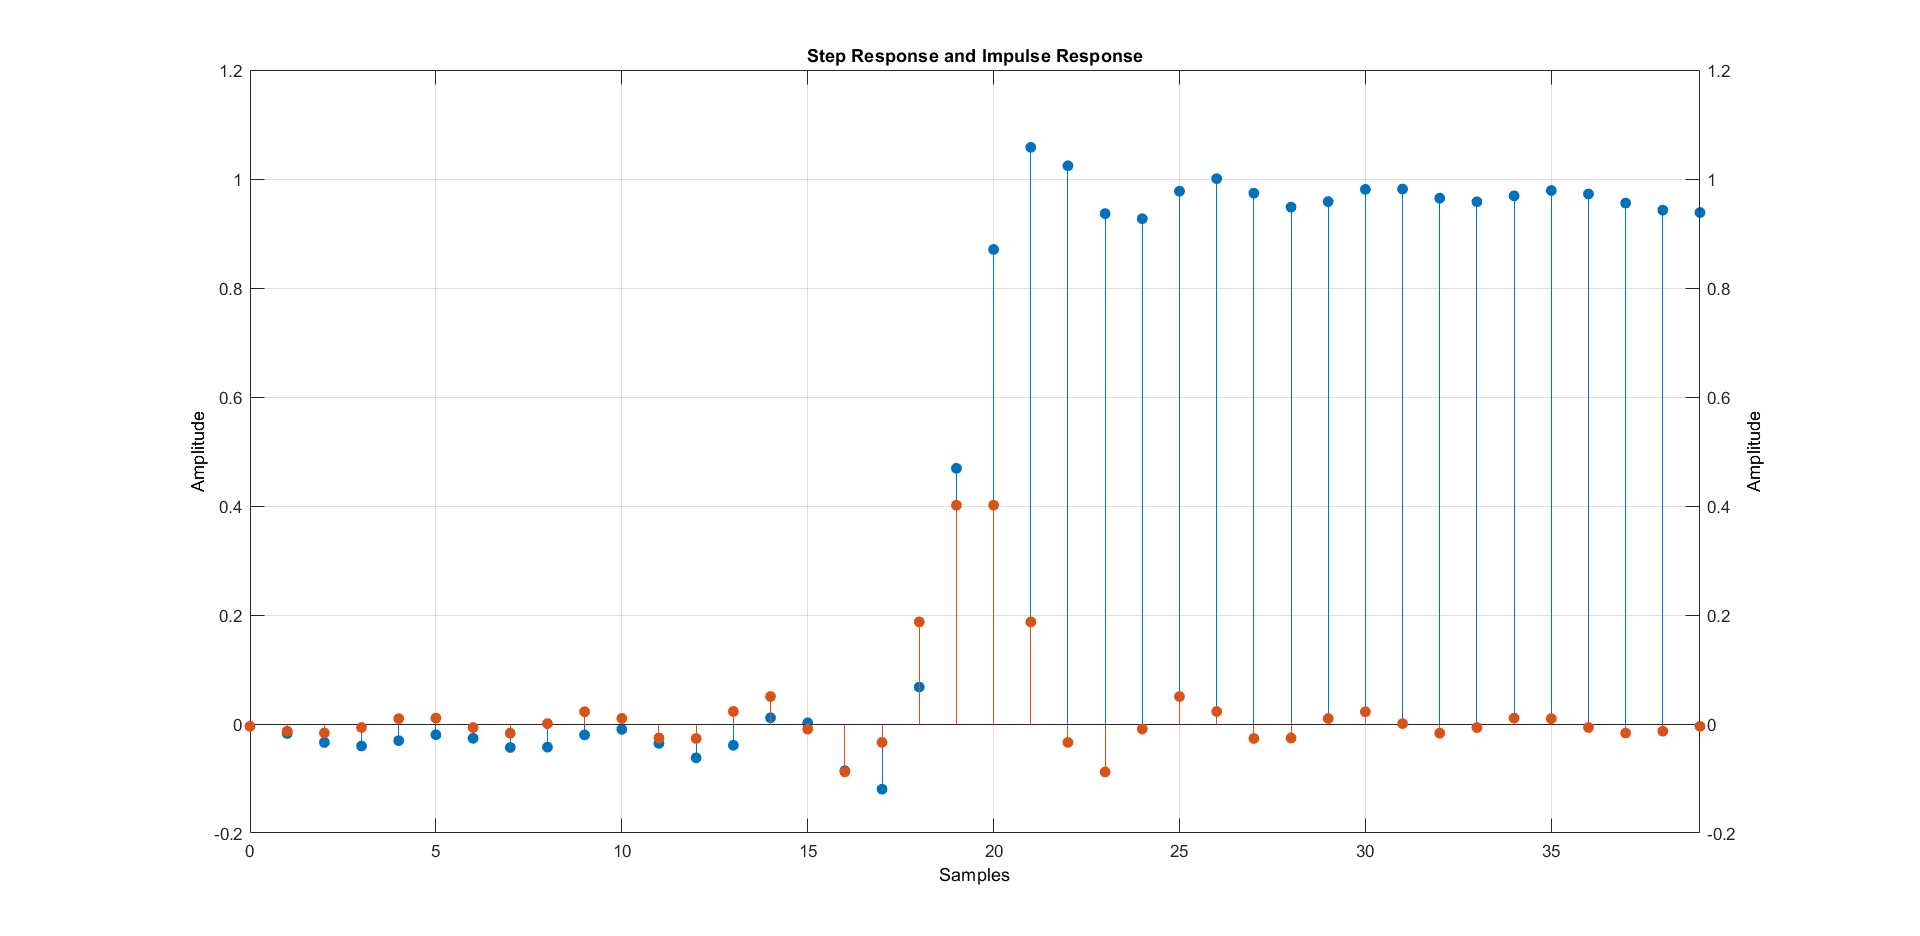
\includegraphics[width=1.0\linewidth]{res/5_fir_time.png}
		\caption{Временные характеристики FIR фильтра}
	\end{figure}
	
	Синтезируем IIR-фильтр Баттерворта нижних частот с теми же характеристиками.
	
	\begin{figure}[H]
		\centering
		\includegraphics[width=1.0\linewidth]{res/5_batt_poles.png}
		\caption{Карта полюсов IIR-фильтра Баттерворта}
	\end{figure}
	
	\begin{figure}[H]
		\centering
		\includegraphics[width=1.0\linewidth]{res/5_batt_ach.png}
		\caption{Частотные характеристики IIR-фильтра Баттерворта}
	\end{figure}
	
	\begin{figure}[H]
		\centering
		\includegraphics[width=1.0\linewidth]{res/5_batt_time.png}
		\caption{Временные характеристики IIR-фильтра Баттерворта}
	\end{figure}
	
	Синтезируем IIR-фильтр Чебышева I типа нижних частот с теми же характеристиками.
		
	\begin{figure}[H]
		\centering
		\includegraphics[width=1.0\linewidth]{res/5_cheb1_poles.png}
		\caption{Карта полюсов IIR-фильтра Чебышева I}
	\end{figure}
	
	\begin{figure}[H]
		\centering
		\includegraphics[width=1.0\linewidth]{res/5_cheb1_ach.png}
		\caption{Частотные характеристики IIR-фильтра Чебышева I}
	\end{figure}
	
	\begin{figure}[H]
		\centering
		\includegraphics[width=1.0\linewidth]{res/5_cheb1_time.png}
		\caption{Временные характеристики IIR-фильтра Чебышева I}
	\end{figure}

	Синтезируем IIR-фильтр Чебышева II типа нижних частот с теми же характеристиками.
	
	\begin{figure}[H]
		\centering
		\includegraphics[width=1.0\linewidth]{res/5_cheb2_poles.png}
		\caption{Карта полюсов IIR-фильтра Чебышева II}
	\end{figure}
	
	\begin{figure}[H]
		\centering
		\includegraphics[width=1.0\linewidth]{res/5_cheb2_ach.png}
		\caption{Частотные характеристики IIR-фильтра Чебышева II}
	\end{figure}
	
	\begin{figure}[H]
		\centering
		\includegraphics[width=1.0\linewidth]{res/5_cheb2_time.png}
		\caption{Временные характеристики IIR-фильтра Чебышева II}
	\end{figure}
	
	Синтезируем эллиптический IIR-фильтр нижних частот с теми же характеристиками.
		
	\begin{figure}[H]
		\centering
		\includegraphics[width=1.0\linewidth]{res/5_ellp_poles.png}
		\caption{Карта полюсов эллиптического IIR-фильтра}
	\end{figure}
	
	\begin{figure}[H]
		\centering
		\includegraphics[width=1.0\linewidth]{res/5_ellp_ach.png}
		\caption{Частотные характеристики эллиптического IIR-фильтра}
	\end{figure}
	
	\begin{figure}[H]
		\centering
		\includegraphics[width=1.0\linewidth]{res/5_ellp_time.png}
		\caption{Временные характеристики эллиптического IIR-фильтра}
	\end{figure}
	
	
	Синтезируем фильтры нижних частот (FIR-фильтр, фильтр Баттерворта, фильтры Чебышева I и II типов, эллиптический фильтр) с характеристиками:
	$$ wpass = 0.3 \qquad wstop = 0.5 \qquad Apass = 1 \qquad Astop = 80$$

	\begin{figure}[H]
		\centering
		\includegraphics[width=1.0\linewidth]{res/5_2_fir_poles.png}
		\caption{Карта полюсов FIR фильтра}
	\end{figure}
	
	\begin{figure}[H]
		\centering
		\includegraphics[width=1.0\linewidth]{res/5_2_fir_ach.png}
		\caption{Частотные характеристики FIR фильтра}
	\end{figure}

	
	\begin{figure}[H]
		\centering
		\includegraphics[width=1.0\linewidth]{res/5_2_batt_poles.png}
		\caption{Карта полюсов IIR-фильтра Баттерворта}
	\end{figure}
	
	\begin{figure}[H]
		\centering
		\includegraphics[width=1.0\linewidth]{res/5_2_batt_ach.png}
		\caption{Частотные характеристики IIR-фильтра Баттерворта}
	\end{figure}

	
	\begin{figure}[H]
		\centering
		\includegraphics[width=1.0\linewidth]{res/5_2_cheb1_poles.png}
		\caption{Карта полюсов IIR-фильтра Чебышева I}
	\end{figure}
	
	\begin{figure}[H]
		\centering
		\includegraphics[width=1.0\linewidth]{res/5_2_cheb1_ach.png}
		\caption{Частотные характеристики IIR-фильтра Чебышева I}
	\end{figure}

	
	\begin{figure}[H]
		\centering
		\includegraphics[width=1.0\linewidth]{res/5_2_cheb2_poles.png}
		\caption{Карта полюсов IIR-фильтра Чебышева II}
	\end{figure}
	
	\begin{figure}[H]
		\centering
		\includegraphics[width=1.0\linewidth]{res/5_2_cheb2_ach.png}
		\caption{Частотные характеристики IIR-фильтра Чебышева II}
	\end{figure}

	
	\begin{figure}[H]
		\centering
		\includegraphics[width=1.0\linewidth]{res/5_2_ellp_poles.png}
		\caption{Карта полюсов эллиптического IIR-фильтра}
	\end{figure}
	
	\begin{figure}[H]
		\centering
		\includegraphics[width=1.0\linewidth]{res/5_2_ellp_ach.png}
		\caption{Частотные характеристики эллиптического IIR-фильтра}
	\end{figure}
	

\end{document}